% !Tex root = 0A_Manuscript_V1_20240719_ZN.tex

%% 默认博士论文模板 doctor

\documentclass[doctor]{hhuthesis}

%% 模板选项:本科毕业论文bachelor;学术型硕士论文academicmaster;专业学位硕士论文professionalmaster;非全日制专业学位论文nonfulltimemaster;博士论文doctor

%% 更改数学字体设置,Latin Modern Math 默认的有点细,可选用下列宏包
\usepackage[bold-style=ISO]{unicode-math}
\usepackage{fontspec}
\usepackage{unicode-math}
\setmainfont{Times New Roman}
% \setmathfont{TeX Gyre Termes Math}

%% 将所有的ref、cite和超链接修改为蓝色
\usepackage{xcolor}
\let\oldref\ref
\let\oldref\cite
\renewcommand{\ref}[1]{\textcolor{blue}{\oldref{#1}}}
\renewcommand{\cite}[1]{\textcolor{blue}{\oldref{#1}}}
\hypersetup{colorlinks=true, linkcolor=blue, citecolor=blue, urlcolor=blue}

\begin{document}

%% 修改公式中的字体


% 封面
% %%
%封面
%%

%国家图书馆封面和中文信息封面
\studentnumber{210801010002}
\classification{TV14}
\securitylevel{无}
\udc{627}
\title{全球陆地水循环演变特征及未来趋势预测}
\vtitle{全球陆地水循环演变特征及未来趋势预测}
\author{宁忠瑞}

%专业型硕士\tutorinfoa填写学校指导老师信息,\tutorinfob填写基地指导老师信息
%其余用户\tutorinfoa填写指导老师姓名&职称,\tutorinfob填写指导老师单位&地址
\tutorinfoa{张建云\hspace{1em}院士\hspace{1em}博导\hspace{2em}河海大学水文水资源学院}
\tutorinfob{王国庆\hspace{1em}教授\hspace{1em}博导\hspace{2em}河海大学水文水资源学院}

\degree{工学博士}
\major{水文学及水资源}
\submitdate{2016年7月6日}
\defenddate{2016年9月30日}
\awarded{河~海~大~学\hspace{3em}2016年12月30日}
\chairman{王继承}

%%博士答辩专家为7人,硕士答辩专家为5人,\reviewerf{}和\reviewerg{}可以省略不填。
\reviewera{王继承}
\reviewerb{李生柱}
\reviewerc{徐鹏飞}
\reviewerd{陈\hspace{1em}诚}
\reviewere{吴树人}
\reviewerf{姜大文}
\reviewerg{蒋小为}
\nlcdate{2016年12月}
\nlclocate{中~~国~~$\cdot$~~南~~京}
\institute{河海大学}
\zhtitle{河网地区水力水质特性的组合单元解法及反问题的研究}
\zhsubtitle{无}
\entitle{\hfill Combined Cells Model of Hydraulics and Water Quality of \\River Networks and Its Reverse Problem}
\ensubtitle{None}
\thesislang{汉语}
\abstractlang{汉、英}
\thesispages{198}
\numofwords{11}
\thesiskeywords{河网、力特征、水质特性、污染面、联合解法}
\researchfield{工程水力学及环境水力学}

%博士、学术型硕士填写,专业型硕士不用填写
\tutor{张建云~院士}	
\tutorinstitute{河海大学水文水资源学院}

%专业型硕士填写,其余不用填写
\tutora{}
\tutorainstitute{}
\tutorb{}
\tutorbinstitute{}

%英文信息封面
\englishtitle{Combined Cells Model of Hydraulics and Water Quality of River Networks and Its Reverse Problem}
\englishauthor{Ning Zhongrui}
\entutor{Professor~~Zhang Jianyun}
\eninstitute{Hohai University}
\englishdepartment{College of Water Conservancy and Hydropower Engineering}
\englishdate{September, 2016}
\enlocate{Nanjing,  P.R.China}
\englishdegree{Doctor of Engineering}

%制作国家图书馆封面
\makenlctitle

%制作书脊
\makeverticaltitle

%制作中文信息封面
\makeinfo

%制作英文信息封面
\makeeninfo

%论文原创性声明和使用授权
\makedeclare

% %%
% %% 前置部分
% %%
% \frontmatter

% %% 前言,硕士论文不需要可删除
% %%
%% This is file 'preface.tex'
%% It is included by hhuthesis-example.tex for hhuthesis.
%%
%% Copyright(C) 2020-2021, Wenhan Cao
%% College of Water Conservancy and Hydropower Engineering, Hohai University.
%%
%% Version:v2.0.0
%% Last update: April 7th, 2021.
%%
%% Home Page of the Project: https://github.com/caowenhan/thesis
%%
%% This file may be distributed and / or modified under the conditions of the
%% LaTeX Project Public License, either version 1.3c of this license or (at your
%% option) any later version. The latest version of this license is in:
%%
%% http://www.latex-project.org/lppl.txt
%%
%% and version 1.3c or later is part of all distributions of LaTeX version
%% 2008/05/04 or later.
%%
\begin{preface}
	本文结合江苏省八五科技攻关项目,对平原河网水力及水质特性数值模拟的正问题及反问题进行了系统深入的研究……\par
	……\par
	……\par		
\begin{enumerate}
	\item[(1)] 平原河网水力及水质特性数值模拟的正问题。
	\item[(2)] 平原河网水力及水质特性数值模拟的反问题。
\end{enumerate}
	
\end{preface}

% %% 摘要
% %% This is file 'abstract.tex'
%% It is included by hhuthesis-example.tex for hhuthesis.
%%
%% Copyright(C) 2020-2021, Wenhan Cao
%% College of Water Conservancy and Hydropower Engineering, Hohai University.
%%
%% Version:v2.0.0
%% Last update: April 7th, 2021.
%%
%% Home Page of the Project: https://github.com/caowenhan/thesis
%%
%% This file may be distributed and / or modified under the conditions of the
%% LaTeX Project Public License, either version 1.3c of this license or (at your
%% option) any later version. The latest version of this license is in:
%%
%% http://www.latex-project.org/lppl.txt
%%
%% and version 1.3c or later is part of all distributions of LaTeX version
%% 2008/05/04 or later.
%%

\begin{abstract}
	本文首次提出并建立了诸如组合单元水力计算正问题、组合单元水质正问题、水量模型参数反问题、水质边界条件及污染源项反问题等系列成果。主要研究内容如下:
\begin{enumerate}
	\item[(1)] 组合单元水力计算正问题。
	\item[(2)] 组合单元水质正问题。
\end{enumerate}


\keywords{河网;力特征;水质特性;污染面;联合解法}
\end{abstract}

\begin{enabstract}
	This paper makes more systematic and deeper studies on numerical simulations of hydraulics and water quality features of river networks. As a result, a series of achievements such as combined cells model of hydraulics, combined cells model of water quality, roughness parameter reverse problem, waste load reverse problem and simulation of hydraulics boundary condition have been put forward for the first time. The details are as follows:

\begin{enumerate}
\item[(1)] combined cells model of hydraulics.
\item[(2)] combined cells model of water quality.
\end{enumerate}  
 
\enkeywords{River network; Force characteristics; Water quality characteristics; Pollution surface; Joint solution}

\end{enabstract}


% %% 符号对照表,可选,如不用可注释掉
% %% This is file 'denotation.tex'
%% It is included by hhuthesis-example.tex for hhuthesis.
%%
%% Copyright(C) 2020-2021, Wenhan Cao
%% College of Water Conservancy and Hydropower Engineering, Hohai University.
%%
%% Version:v2.0.0
%% Last update: April 7th, 2021.
%%
%% Home Page of the Project: https://github.com/caowenhan/thesis
%%
%% This file may be distributed and / or modified under the conditions of the
%% LaTeX Project Public License, either version 1.3c of this license or (at your
%% option) any later version. The latest version of this license is in:
%%
%% http://www.latex-project.org/lppl.txt
%%
%% and version 1.3c or later is part of all distributions of LaTeX version
%% 2008/05/04 or later.
%%

\begin{denotation}
	
\item[\LaTeX] 一个很棒的排版系统
\item[\LaTeXe] 一个很棒的排版系统的最新稳定版
\item[\XeTeX] \LaTeX{}的好兄弟,事实上他有很多个兄弟,但是这个兄弟对各种语言的支持能力都很强
\item[ctex] 成套的中文\LaTeX{}解决方案
\item[\ce{CaCO3}] 碳酸钙
\item[$ e^{\pi{}i}+1=0$] 集自然界五大常数一体的最美方程,欧拉公式

\end{denotation}


%% 加入目录
\tableofcontents

% %% 加入图、表索引(同时取消图表索引中章之间的垂直间隔,不需要可以注释)
\let\origaddvspace\addvspace
\renewcommand{\addvspace}[1]{}
\listoffigures
\listoftables
\renewcommand{\addvspace}[1]{\origaddvspace{#1}}

%%
%% 正文部分
%%
\mainmatter


%% 各章正文内容
% \chapter{绪论}
\label{chap:introduction}

\section{研究背景及研究意义}

\section{国内外研究现状}

\subsection{全球水循环要素演变分析}

\subsection{水文模型发展研究}

\subsection{水文模型参数区域化研究}

\subsection{未来全球水循环要素变化预测研究}

\subsection{现存问题及发展趋势}

\section{拟解决的科学问题及研究内容}

\section{研究思路与技术路线}

\cleardoublepage
% \chapter{研究流域与数据}
\label{chap:data_and_All_Global_Stations}

\section{研究流域}

本论文各章节采用的研究流域均基于全球径流数据库(Global Runoff Data Base, GRDB),全球径流指数和元数据存档(Global Streamflow Indices and Metadata Archive, GSIM)以及补充的中国流域径流数据221个三部分共同组成。其中,搜集的中国流域的数据目的在于补充全球数据集中在中国记录缺失的空白。

\subsection{全球径流数据集}

全球径流数据库是由世界气象组织(World Meteorological Organization, WMO)于20世纪80年代组织建立的国际数据档案库,其中保存着长达200年的数据,旨在促进促进跨国和全球的水文数据和信息交换,帮助地球科学领域的学者分析全球气候趋势并评估环境影响和风险。GRDB提供的观测径流数据已经被广泛应用于国家、地区和全球尺度的水文分析、模型开发及评估等研究中\cite{burekUseGRDCGauging2023, houGlobalEvaluationRunoff2023}。\par
全球径流数据库最初建立在20世纪80年代初收集的初始数据集上,这些数据集是为了响应世界气象组织的要求,由成员国提供的全球水文数据,以补充第一次全球GARP试验(First Global GARP Experiment, FGGE)框架内的特定大气数据。这些数据集最初包含了1980年前后几年的月尺度径流数据,后来又纳入了联合国教科文组织1965-1985年的月尺度径流数据。在世界气象组织的支持下,经过三十多年的数据收集和质量控制,历史平均每日和每月径流的数据库得以稳步增长,最早的数据可以追溯到1806年,而最新的数据则是近实时更新的。目前,该数据库涵盖了来自全球159个国家和地区的10829个观测站点的每日和每月河流流量时间序列数据,总计约470,000个站点年,平均记录长度为45年,最长纪录长度为217年。数据库中所有的径流观测数据均公开下载(\href{https://grdc.bafg.de/GRDC/EN/02_srvcs/21_tmsrs/210_prtl/prtl_node.html}{https://grdc.bafg.de/GRDC/EN/02\_srvcs/21\_tmsrs/210\_prtl/prtl\_node.html},最后访问时间:2024年7月29日)。\par
此外,GRDB还根据其收集的数据生成各种数据产品,例如长期统计数据和年度特征分析,以及流入世界海洋的表面淡水通量。中心还提供了许多GIS图层,包括各个站点的集水区边界,便于生成地图产品。这些资源大大促进了全球水文和气候研究,使研究人员能够更好地理解和应对全球变化带来的挑战。径流观测站位置如图\ref{fig:All_Global_Stations}(a)所示。\par

GSIM由Do等人创建\cite{doGlobalStreamflowIndices2018, gudmundssonGlobalStreamflowIndices2018},是来自世界各地的每日河流流量现场观测的综合集合,旨在加强对大尺度淡水资源的了解。作为GRDB的扩展,GSIM档案整合包括欧洲径流档案(European Water Archive, EWA),俄罗斯区域水文数据网络(A Regional, Electronic, Hydrographic Data Network for Russia, ARCTICNET),中国水文数据项目(China Hydrology Database Project, CHDP),美国国家水信息系统(US National Water Information System, USGS)等在内的12个不同来源的数据,并对数据进行了广泛、正式而标准的数据质量控制流程,最终形成了包含30,959个独特的站点的元数据的数据集(\href{https://doi.pangaea.de/10.1594/PANGAEA.887470}{https://doi.pangaea.de/10.1594/PANGAEA.887470},最后访问时间:2024年8月2日)。\par
GSIM数据集包括各种类型的元数据,如站点id、地理坐标、站点海拔、径流指数和集水区边界等。基于观测站的日径流数据,计算出月度、季度和年度三种时间分辨率的流量属性,以及年最大最小值(MAX, MIN)、平均值(MEAN)、第10个百分位数(P10)、中位数(P50)、第90个百分位数(P90)等多种径流指数。基于全球数字高程模型(Digital Elevation Model,DEM)和重新定位算法提取了流域边界,使得用户可以轻松的提取感兴趣的数据,如气候、土壤、土地利用类型等。GSIM数据集已经被广泛应用于全球水文研究、气候变化研究、水资源管理等领域,为全球水文研究提供了重要的数据支持\cite{gudmundssonObservedTrendsGlobal2019}。径流观测站位置如图\ref{fig:All_Global_Stations}(b)所示。\par

\begin{figure}[H]
	\centering
	\includegraphics[width=0.75\textwidth]{figures/chap2/All_Global_Stations.jpg}
	\bicaption{全球径流观测站位置图}{Location of streamflow gauging stations selected from GRDC and GSIM}\label{fig:All_Global_Stations}
\end{figure}

\subsection{中国径流数据集}

在全球径流数据集提供的众多数据中,中国大陆的站点较少,提供了日径流站点仅为26个,且径流数据缺失率高\cite{GouJiaoJiaoJiYuVICDeZhongGuoTianRanJingLiuGuSuanYuPingJie2021},GRDC和GSIM数据集中,中国数据平均缺失率分别为32.5\%和30.2\%。为了使全球径流数据集更加完整,增强研究结果在中国的代表性,需要在GRDC和GSIM数据集的基础上补充中国流域的径流数据。
我国所有流域可以划分为十大一级水资源区,分别是松花江区、辽河区、海河区、黄河区、淮河区、长江区、珠江区、东南诸河区、西南诸河区和西北诸河区。本研究在全国各大流域片区搜集径流数据,包括长江流域、黄河流域在内的共54个站点的月尺度长系列径流观测资料,形成了中国实测径流数据集,以补充全球径流数据在中国地区的记录缺失和空白。各站点坐标如图\ref{fig:All_China_Stations}所示。\par

\begin{figure}[H]
	\centering
	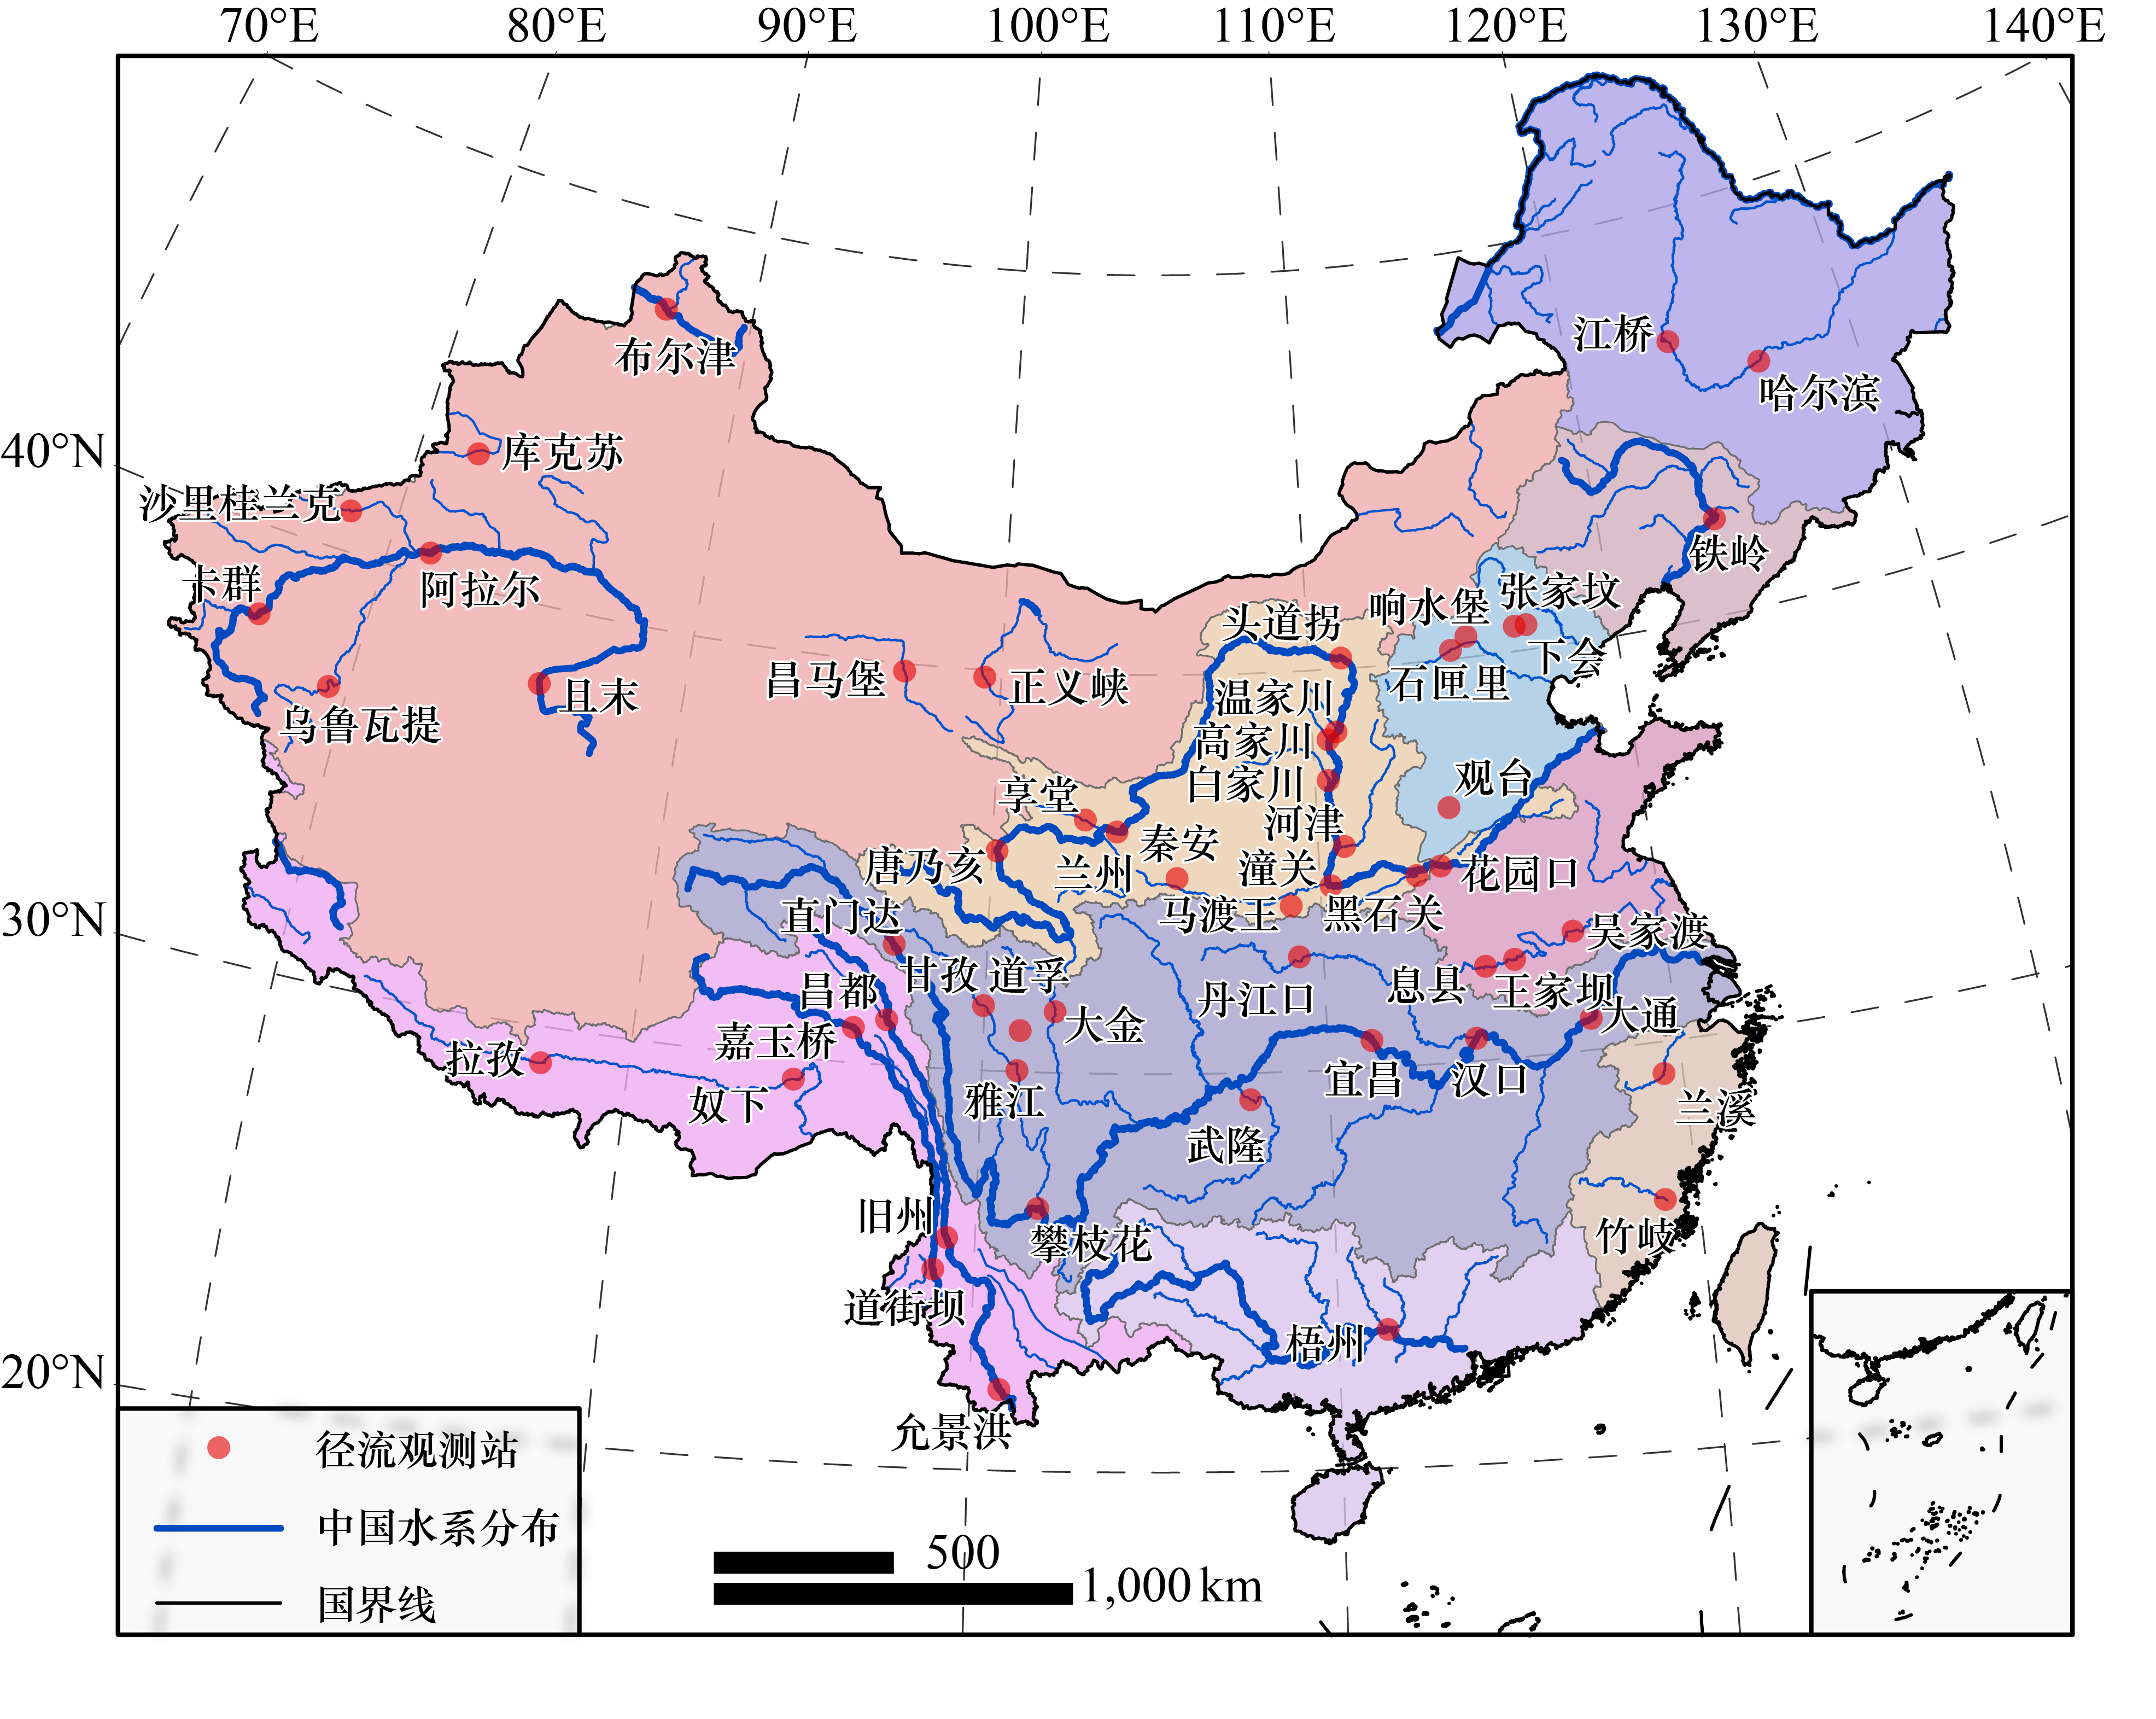
\includegraphics[width=0.85\textwidth]{figures/chap2/China_Stations.jpg}
	\bicaption{中国径流观测站位置图}{Location of Chinese streamflow gauging stations}\label{fig:All_China_Stations}
\end{figure}

\section{研究数据}

论文研究使用的数据包括全球格点尺度上的历史气候学(气温、降水、潜在蒸散发、实际蒸散发、雪水当量)、土壤质地、地形、植被覆盖、径流观测与重建、气候模式输出以及全球陆地分区数据(基于气候条件和基于地理位置的分区)等。这些数据将用于研究全球水文循环历史演变的时空规律、评估与构建全球水文模型以及探究全球水资源对气候变化的相应。表\ref{tab:data}总结了本研究中使用的数据和来源。

\begin{table}[H]\small	%\small用于控制表格内字体大小为5号字
	\centering
	\bicaption{研究使用的气候学、径流和下垫面数据及其来源}{Climatology, runoff and underlying surface data with source used in the research} \label{tab:data}
	\begin{tabular*}{1\textwidth}{@{\extracolsep{\fill}}ccccc}
		\toprule % 第一条线。头部的线
		% 表头
		数据类型 & 数据 & 空间分辨率 & 时间分辨率 & 数据来源 \\
		\midrule % 第二条线,中间的线
		\multirow{8}*{\makecell{历史\\气候条件}} & 降水 & \multirow{3}*{0.5°} & \multirow{3}*{\makecell{1901-2022年\\(月尺度)}} & \multirow{3}*{\makecell{CRU TS v4.07\\气候研究单元时间\\序列数据集}}\\
		~ & 气温 & ~ & ~ & ~ \\
		~ & 潜在蒸散发 & ~ & ~ & ~ \\
		~ & 降水 & \multirow{5}*{0.1°} & \multirow{5}*{\makecell{1951-2024年\\(月尺度)}} & \multirow{5}*{\makecell{ERA5-Land全球气候\\再分析数据集}}\\
		~ & 气温 & ~ & ~ & ~ \\
		~ & 潜在蒸散发 & ~ & ~ & ~ \\
		~ & 实际蒸散发 & ~ & ~ & ~ \\
		~ & 雪水当量 & ~ & ~ & ~ \\
		\midrule % 第二条线,中间的线
		\multirow{7}*{径流} & \multirow{3}*{观测径流} & \multirow{3}*{/} & \multirow{3}*{/} & GRDB全球径流数据库 \\
		~ & ~ & ~ & ~ & \makecell{GSIM全球径流指数\\和元数据存档} \\
		~ & \multirow{2}*{重建径流} & 0.5° & 1902-2014年 & GRUN全球天然径流数据集\\
		~ & ~ & 0.25° & 1961-2018年 & CNRD中国天然径流数据集\\
	    ~ & 径流系数 & \multirow{2}*{0.125°} & \multirow{2}*{/} & \multirow{2}*{全球径流特征数据集(GSCD)} \\
		~ & 基流系数 & ~ & ~ & ~\\
		\midrule % 第二条线,中间的线
		植被特征 & \makecell{归一化植被\\指数NDVI} & 1/12° & 15天 & \makecell{全球模拟和绘图项目(GIMMS)}\\
		\midrule % 第二条线,中间的线
		\multirow{7}*{下垫面} & 高程 & 30米 & / & \makecell{ASTER全球数字高程地图} \\
		~ & 土壤质地 & 30弧度秒 & / & \makecell{联合国粮食及农业组织\\世界土壤数据库(HWSDv1.2)} \\
		~ & 土地利用类型 & 1千米 & / & \makecell{马里兰大学(UMD)\\土地利用数据集} \\
		~ & 流向 & 0.5° & / & \makecell{国际卫星陆地表面气候学\\计划II(ISLSCP II)河流路由数据} \\
		\bottomrule % 第三条线,底部的线
	\end{tabular*}%
\end{table}

\subsection{历史气候再分析数据}

气候研究单元时间序列数据集(Climatic Research Unit Time Series,CRU TS)是英国国家大气科学中心(UK National Centre for Atmospheric Science,NCAS)及其合作者开发的全球历史气候格点再分析数据集(\href{https://crudata.uea.ac.uk/cru/data/hrg/cru_ts_4.07/}{https://crudata.uea.ac.uk/cru/data/hrg/cru\_ts\_ 4.07/},最后访问时间:2024年8月2日)\cite{harrisVersionCRUTS2020}。数据集收集广泛的气象站点观测网络的每月气候数据,有10种变量,分别是近地表气温(最高、最低、平均和昼夜温差)、降水量(总降水量、降水天数)、湿度(蒸汽压)、潜在蒸散发、云量、霜天数等,通过角距离加权(Angular-Distance Weighting,ADW)算法进行插值,以0.5°×0.5°经纬度网格覆盖全球除南极洲以外的世界所有陆地区域,并且每年进行一次更新,目前的数据序列可以覆盖从1901至2022年,是目前可获得的最长数据序列的历史气候再分析数据集。\par

ERA5-Land是欧洲中期天气预报中心(European Centre for Medium-Range Weather Forecasts,ECMWF)在欧盟委员会哥白尼气候变化服务(Copernicus Climate Change Service,C3S)的框架内开发的第五代全球气候再分析数据集(\href{https://cds.climate.copernicus.eu/cdsapp#!/dataset/reanalysis-era5-land-monthly-means?tab=overview}{https://cds.climate.cop ernicus.eu/cdsapp\#!/dataset/reanalysis-era5-land-monthly-means?tab=overview},最后访问时间:2024年8月2日)\cite{hersbachERA5GlobalReanalysis2020,munoz-sabaterERA5LandStateoftheartGlobal2021}。与ERA5相比,它以更高的分辨率提供了数十年来陆地变量演变的一致视图。ERA5-Land是通过气候强迫驱动ECMWF ERA5物理模型的陆地部分进行重新计算而生成的,并进行了热力学近地表状态的高程校正。模型利用物理定律将模型数据与来自世界各地的观测结果相结合,形成一个全球水和能源演变的完整且一致的数据集。数据集包括了多种气象要素,如气温、降水、潜在蒸散发、实际蒸散发、雪水当量等,以0.1°×0.1°经纬度网格覆盖全球陆地区域,时间分辨率为小时和月,时间范围从1951年至今。ERA5-Land以其高时空分辨率支持设计水资源、土地和环境管理的各种应用。\par

\subsection{网格径流数据}

在分布式水文模型的应用过程中,当仅使用出口站点的径流数据时,集水区范围内的空间异质性被均化处理,无法提供空间模式信息。相较于站点观测径流数据,网格化数据以其相对统一的空间分辨率、对非自然流域描述的高自由度,被广泛应用于大尺度研究中。\par

\subsubsection{全球网格径流数据}

全球格点径流数据集(Global Gridded Runoff Dataset,GRUN)是一个基于观测径流数据的全球网格化重建径流数据集(\href{https://figshare.com/articles/dataset/GRUN_Global_Runoff_Reconstruction/9228176}{https://figshare.com/articles/dataset/GRUN\_Global \_Runoff\_Reconstruction/9228176},最后访问时间:2024年8月2日),由Ghiggi等人开发\cite{ghiggiGRUNObservationbasedGlobal2019, ghiggiGRUNENSEMBLEMultiForcing2021}。原位观测径流被用于训练机器学习算法,根据大气再分析中的前期气温和降水来预测月径流,并进行交叉验证评估,并与大型河流的一组独立的径流观测数据进行比较。与13个最先进的全球水文模型径流模拟的集合相比,GRUN具有更好的平均一致性和更低的不确定性。GRUN数据集提供了全球0.5°×0.5°经纬度网格的月尺度径流数据,时间范围为1902-2014年。该数据集被广泛应用于全球淡水动态、年际变化、干旱传播以及径流对大气遥相关的响应等方面的研究。\par

\subsubsection{全球网格径流特征数据}

全球径流特征图(Global Streamflow Characteristics Dataset,GSCD)包含17种径流特征的全球地图,例如基流指数、径流系数和流量百分位数,提供有关整个陆地表面(包括未测量区域)径流行为的信息\cite{beckGlobalPatternsBase2013, beckGlobalMapsStreamflow2015},通过GloH2O发布(\href{https://www.gloh2o.org/gscd/}{https://www.gloh2o.org/gscd/},最后访问时间:2024年8月2日)。利用全球超过3000个中小型流域(集水区面积介于10-10000千米\textsuperscript2之间)观测到的日径流资料训练集合神经网络,以根据流域的气候和地貌特征估计径流特征参数。经过训练的集合神经网络被应用在整个无冰陆面上,以生成全球0.125°×0.125°网格上的径流特征地图。

\subsubsection{中国网格径流数据}

中国天然径流数据集(China Natural Runoff Dataset,CNRD)是由北京师范大学Gou等\cite{gouCNRDV1HighQuality2021, gouSensitivityAnalysisBased2020, gouSeasonalityImpactFactor2022, GouJiaoJiaoJiYuVICDeZhongGuoTianRanJingLiuGuSuanYuPingJie2021}人开发的覆盖中国大陆的质量控制的历史网格化天然径流重建数据集(\href{https://figshare.com/articles/dataset/CNRDv1_0/13185410}{https:// figshare.com/articles/dataset/CNRDv1\_0/13185410},最后访问时间:2024年8月2日)。数据集提供了1961-2018年期间中国的日、月和年0.25°×0.25°径流估算。CNRD使用可变下渗容量模型(Variable Infiltration Capacity,VIC)生成,利用超过200个自然或接近自然的标准集水区训练模型,并结合参数敏感性分析、优化和区域化框架以提高产品稳健性。CNRD是中国第一个使用不确定性框架估算网格化天然径流的数据集,为大尺度径流估算提供了重要的数据和方法参考。\par

\begin{figure}[H]
	\centering
	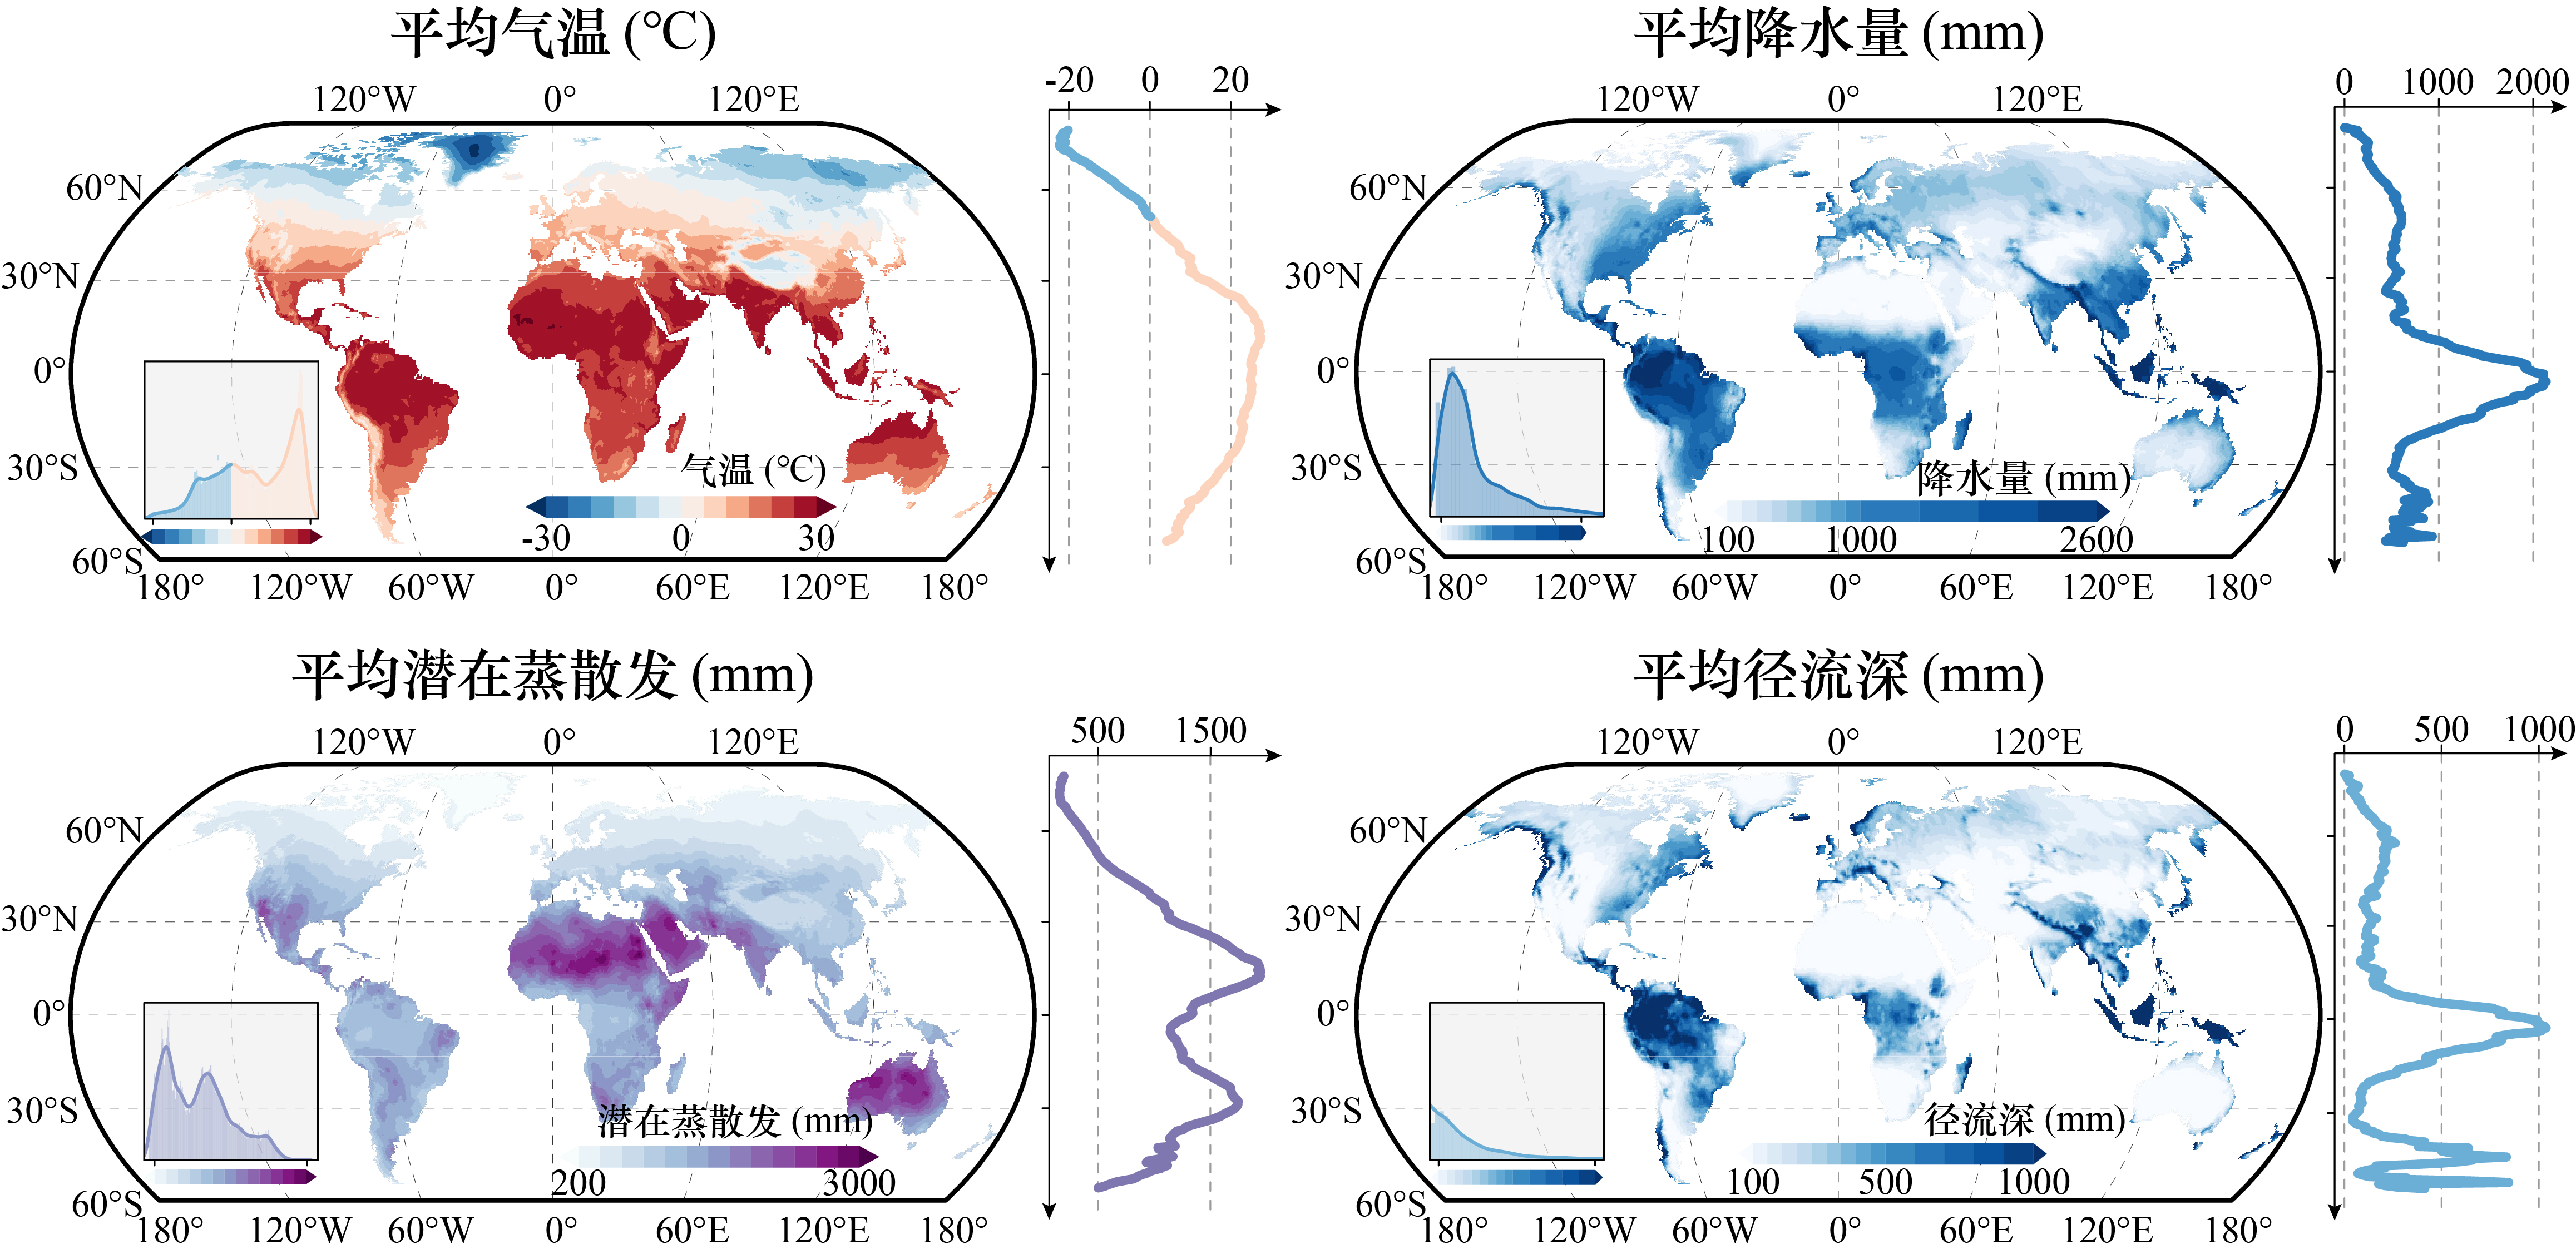
\includegraphics[width=1\textwidth]{figures/chap2/Global_Ave_Climatic.jpg}
	\bicaption{全球历史气候与径流数据}{Global historical climatic and runoff data}\label{fig:Global_Climatic_Data}
\end{figure}

\subsection{下垫面数据}

本论文使用的下垫面数据包括高程、土壤质地、流向和植被覆盖等。下垫面条件的空间异质性对流域水循环过程有重要的影响,因此需要在水文模型中考虑下垫面条件的时空分异模式。

\subsubsection{高程数据}

数字高程模型(Digital Elevation Model,DEM)是对地表地形的数字表示。本研究采用的DEM数据来源于日本经济产业省(Ministry of Economy,Trade,and Industry of Japan,METI)与美国国家航空航天局(United States National Aeronautics and Space AdministrationNASA)联合发布的先进星载热发射和反射辐射计(Advanced Spaceborne Thermal Emission and Reflection Radiometer,ASTER)全球数字高程模型第3版(GDEM v003)。ASTER GDEM是通过ASTER传感器在2000年至2011年间的卫星影像数据生成的,覆盖范围从北纬83°到南纬83°,涵盖了地球99\%的陆地面积,空间分辨率为30米,并且具有1°×1°的图块。该DEM数据广泛应用于地理信息系统、环境监测、自然灾害评估、地质研究等领域。数据在NASA的数据网站Earthdata(\href{https://search.earthdata.nasa.gov/search/}{https://search.earthdata.nasa.gov/search/},最后访问时间:2024年8月2日)上提供公开下载。

\subsubsection{土壤质地数据}

土壤质地是对土壤颗粒组成的描述。联合国粮食及农业组织(Food and Algriculture Organization,FAO)联合国际应用系统分析研究所(International Institute for Applied Systems Analysis,IIASA)、中国科学院南京土壤研究所(Institute of Soil Science,Chinese Academy of Sciences,ISSCAS)和欧盟委员会联合研究中心(Joint Research Centre of the European Commission,JRC)发布了全球30弧度秒分辨率的世界土壤数据库(Harmonized World Soil Database,HWSD v1.2)。该数据库包含超过15,000个不同的土壤测绘单元,综合了现有世界各区域和国家更新的土壤信息,并进行统一标准的分类,使用标准化结构将属性数据与栅格地图联系起来。土壤特征参数主要包括有机碳,pH值,土壤深度,土壤类型,砂土、壤土、粘土三种组分含量,土壤质地等。其中土壤质地由土壤三种组分含量通过美国农业部(US Department of Agriculture,USDA)的土壤质地分类三角(Soil Texture Classification Triangle)进行划分,分为砂土、壤土等12种类型\cite{moreno-marotoEvaluationUSDASoil2022}。数据在FAO网站上(\href{https://www.fao.org/soils-portal/data-hub/soil-maps-and-databases/harmonized-world-soil-database-v12/en/}{https://www.fao.org/soils-portal/data-hub/soil-maps-and-databases/harmonized-world-soil-database-v12/en/},最后访问时间:2024年8月2日)提供公开下载。

\subsubsection{流向数据}

模拟拓扑网络(Simulated Topological Network,STN-30p)为分布式水文模型构建提供了全球河流系统的精确表示,包括全球0.5°网格上的流向、河道长度、河道等级等信息。STN-30p数据集为每个陆地网格单元分配了8个可能的流向之一,来表明陆地之间的潜在连通性。数据集由国际卫星陆地表面气候学计划II(International Satellite Land Surface Climatology Project II,ISLSCP II)发布(\href{https://daac.ornl.gov/cgi-bin/dsviewer.pl?ds_id=1005}{https://daac.ornl.gov/cgi-bin/dsviewer.pl?ds\_id=1005},最后访问时间:2024年8月2日)。

\subsubsection{植被覆盖数据}

流域植被覆盖与降水冠层截留、植被蒸腾作用密切相关。归一化植被指数(NormalizedDifference Vegetation Index, NDVI)是植被冠层绿叶中叶绿素吸收的光合有效辐射的辐射测量,是反映流域植被特征的重要指标。NDVI值的范围为1.0到-1.0。贫瘠的岩石、沙地或积雪区域通常显示非常低的NDVI值(0.1或更低)。稀疏的植被(例如灌木和草地)或衰老的作物可能导致中等的NDVI值(大约0.2到0.5)。高NDVI值(大约0.6到0.9)对应于茂密的植被,例如温带和热带森林中的植被或处于生长高峰期的作物。\par
本研究使用的NDVI数据来自全球模拟和绘图项目(Global Inventory Modeling and Mapping Studies,GIMMS)发布的15天间隔的1/12°分辨率的NDVI数据集(\href{https://www.ncei.noaa.gov/data/land-normalized-difference-vegetation-index/access/}{https://www.ncei.noaa.gov/data/land-normalized-difference-vegetation-index/access/},最后访问时间:2024年8月2日)。该数据集基于NASA的先进非扫描辐射计(Advanced Very High Resolution Radiometer,AVHRR)传感器,经过辐射校正和坐标转换,并消除由于轨道偏移等偏差后发布,覆盖了1981年7月至今的全球陆地表面,提供了全球植被覆盖的时空变化信息。

\begin{figure}[H]
	\centering
	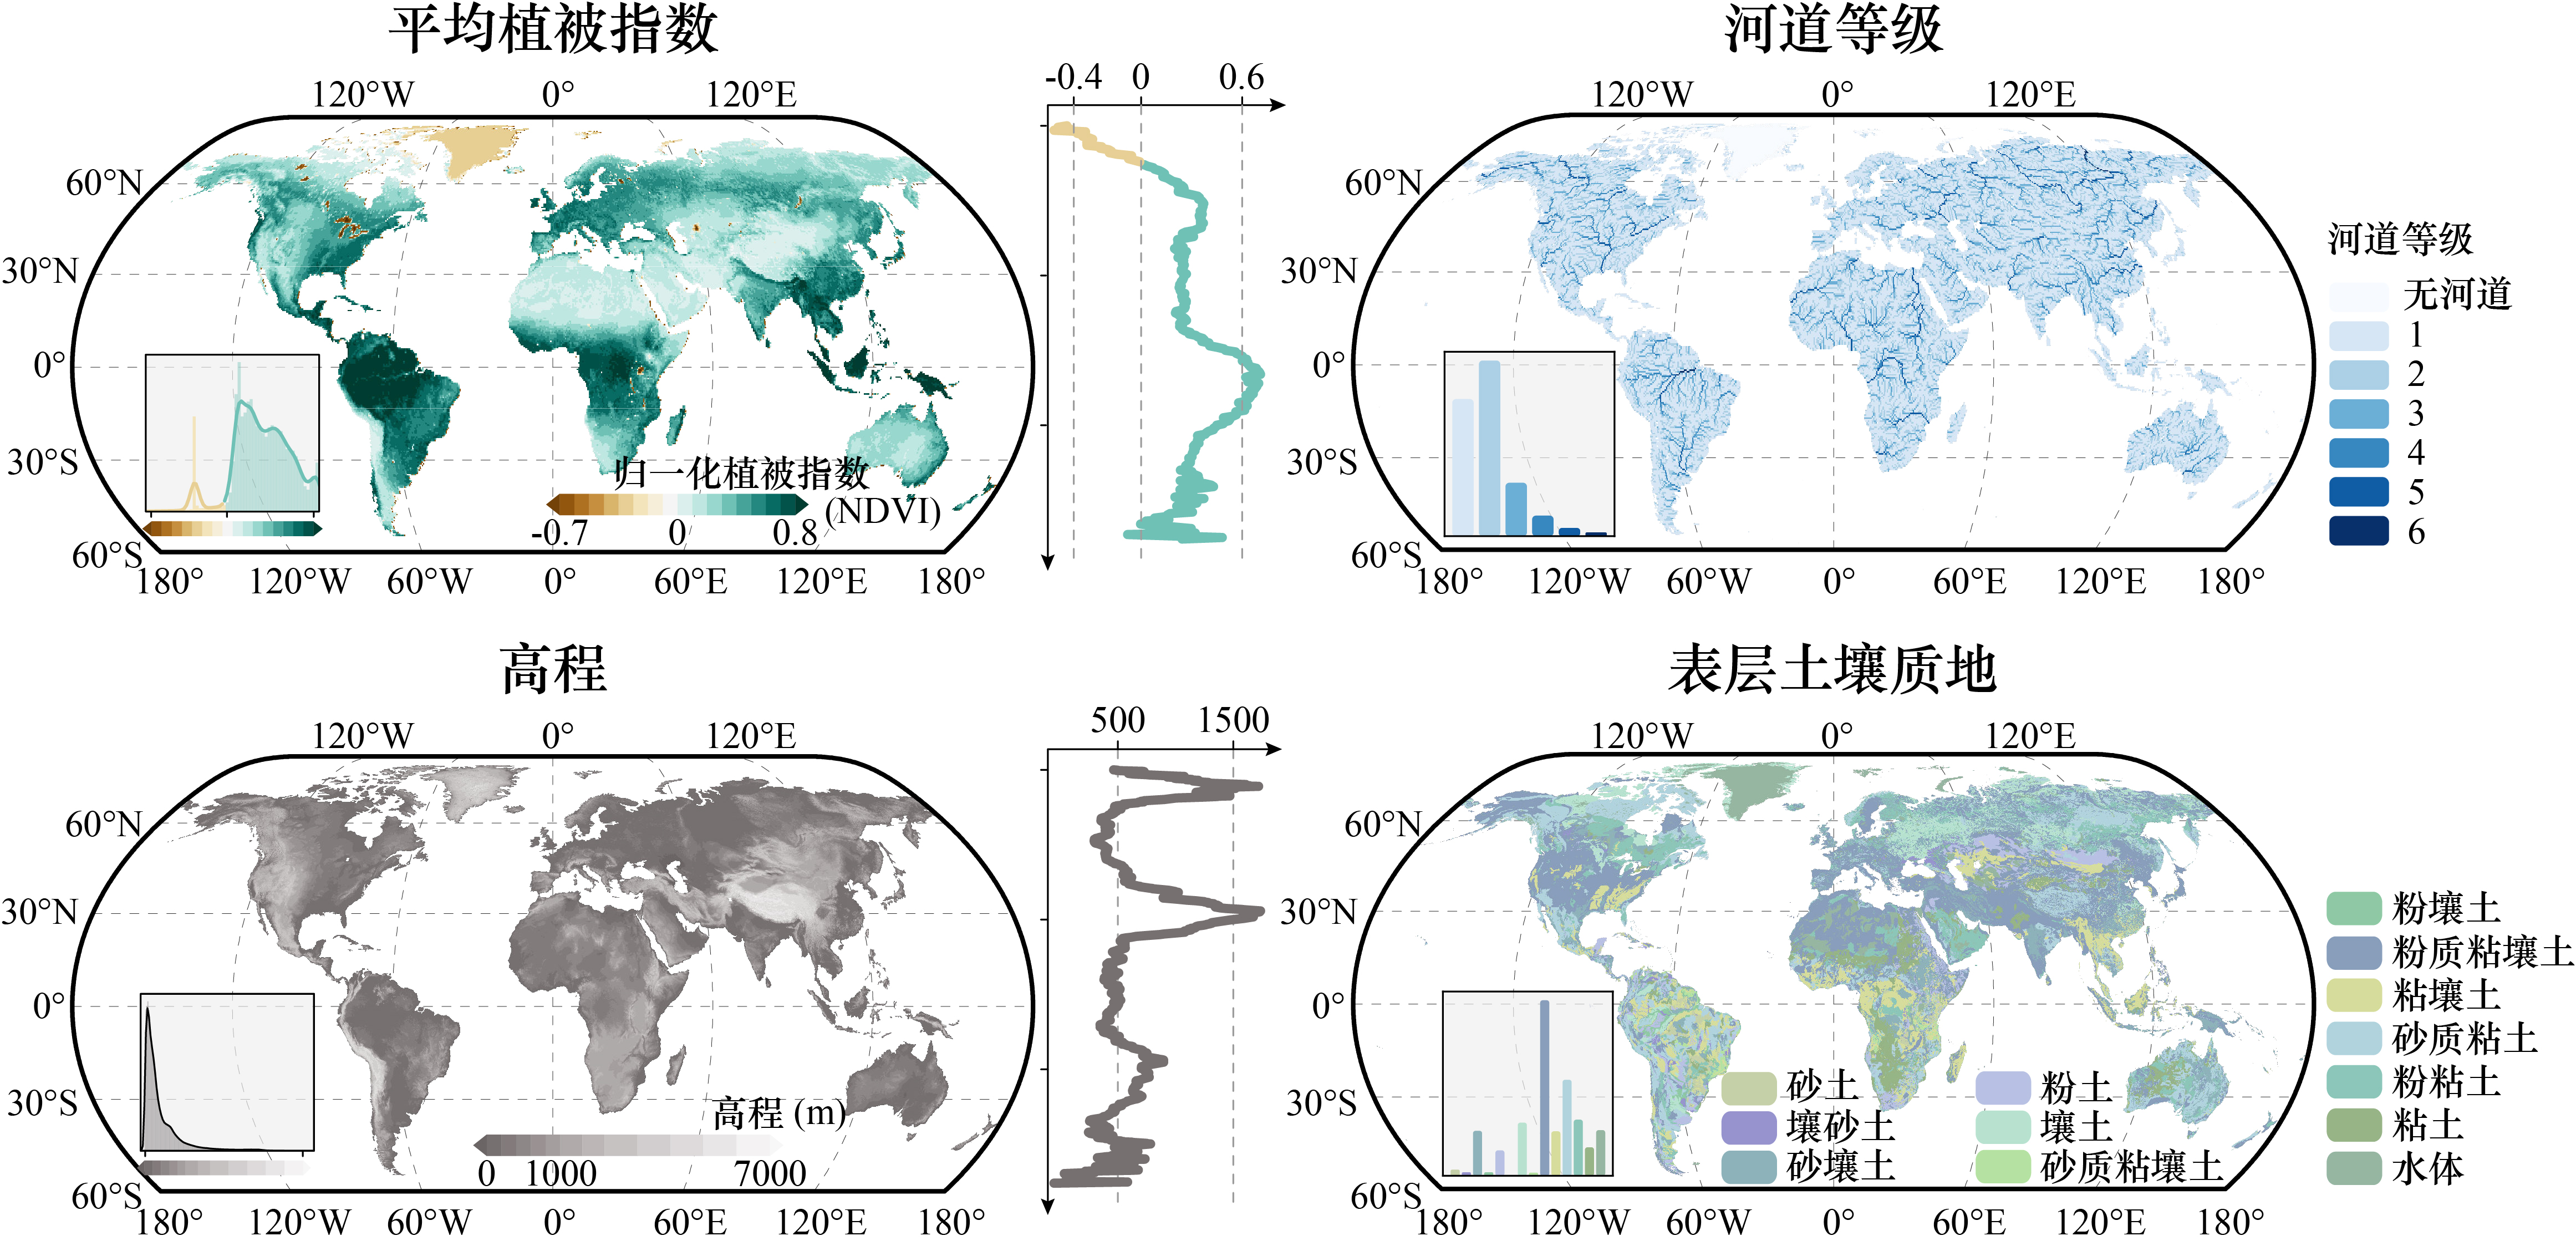
\includegraphics[width=1\textwidth]{figures/chap2/Global_Underlying.jpg}
	\bicaption{全球陆地下垫面数据}{Underlying surface data of global land}\label{fig:Global_Underlying_Data}
\end{figure}

\subsection{气候模式数据}

全球气候模型(Global Climate Model,GCM)是一种用于模拟全球气候系统的数值模型,是研究全球气候变化的重要工具。GCM利用一系列的数学公式来描绘气候系统的各个主要组成部分,包括大气、海洋、冻土以及地表和海洋表面的生物地理过程。世界气候研究计划组织(World Climate Research Programme,WCRP)自20世纪90年代起组织了一系列的耦合模式比较计划(Coupled Model Intercomparison Project,CMIP),目前已经发展到第六阶段(CMIP6)。CMIP6的目标是为全球气候变化研究提供最新的全球气候模型模拟数据,以评估全球气候模型的性能,分析全球气候变化的趋势\cite{ZhouTianJunDiLiuCiGuoJiOuHeMoShiBiJiaoJiHuaCMIP6PingShu2019}。作为CMIP6的一部分,每个模型都提供了1850-2014的历史气候情况模拟及2015-2100年的未来气候预测\cite{ningWetterTrendSource2024}。\par
本研究使用的气候模型数据来自共享社会路径(Shared Socioeconomic Pathways,SSP)下的四种情景,分别是绿色发展路径(SSP1-2.6)、中间路径(SSP2-4.5),区域对抗路径(SSP3-7.0)和化石燃料路径(SSP5-8.5)试验下的全球月尺度气温、降水和太阳辐射强度输出,采用了来自CMIP6的17种GCM输出数据(\href{https://esgf-node.ipsl.upmc.fr/search/cmip6-ipsl/}{https://esgf-node.ipsl.upmc.fr/search/cmip6-ipsl/})。表\ref{tab:gcmdata}汇总了所选GCM模型的具体信息。

\begin{table}[H]\small	%\small用于控制表格内字体大小为5号字
	\centering
	\bicaption{本研究中使用的未来气候模式信息}{Global climate models used in the research} \label{tab:gcmdata}
	\begin{tabular*}{0.9\textwidth}{@{\extracolsep{\fill}}cccc}
		\toprule % 第一条线。头部的线
		% 表头
		序号 & 气候模式 & 研发机构/地区 & 空间分辨率 \\
		\midrule % 第二条线,中间的线
		1 & ACCESS-CM2 & \multirow{2}*{CSIRO/澳大利亚} & \multirow{2}*{1.875°×1.25°} \\
        2 & ACCESS-ESM1-5 & ~ & ~ \\
        3 & BCC-CSM2-MR & BCC/中国 & 1.125°×1.125° \\
        4 & CanESM5 & CCCma/加拿大 & 2.8125°×2.8125° \\
        5 & CAS-ESM2-0 & CAS/中国 & 1°×1° \\
        6 & EC-Earth3 & \multirow{2}*{\makecell{EC-Earth-Consortium\\瑞典}} & \multirow{2}*{0.703°×0.703°} \\
        7 & EC-Earth3-Veg-LR & ~ & ~ \\
        8 & FIO-ESM-2-0 & CAS/中国 & 1°×1° \\
        9 & GFDL-CM4 & NOAA-GFDL/美国 & 1°×1.25° \\
        10 & INM-CM4-8 & \multirow{2}*{INM/俄罗斯} & \multirow{2}*{2°×1.5°} \\
        11 & INM-CM5-0 & ~ & ~ \\
        12 & IPSL-CM6A-LR & IPSL/法国 & 1.5°×1.25° \\
        13 & MIROC6 & MIROC/日本 & 1.40625°×1.40625° \\
        14 & MPI-ESM1-2-HR & \multirow{2}*{MPI-M/德国} & 0.9375°×0.9375° \\
        15 & MPI-ESM1-2-LR & ~ & 1.875°×1.8625° \\
        16 & MRI-ESM2-0 & MRI/日本 & 1.125°×1.125° \\
        17 & NESM3 & NUIST/中国 & 1.875°×1.865° \\
		\bottomrule % 第三条线,底部的线
	\end{tabular*}%
\end{table}

\subsection{全球分区数据}

本研究使用不同类型的全球陆地分区数据评估全球历史水文气候条件演变特征以及各种模型的性能规律。

\subsubsection{全球气候分区数据}

柯本气候分区是目前最常用的气候分类方法之一,主要根据当地气候条件和植被类型对世界各地的气候区进行分类\cite{peelUpdatedWorldMap2007,beckPresentFutureKoppenGeiger2018}。首先根据全球气候将陆地划分为五个主气候带,分别是赤道带(A,最低气温高于18℃),干旱带(B,年降水量低于10倍降水阈值),暖温带(C,最热月气温高于10℃且最冷月气温介于0-18℃之间),亚寒带(D,最热月气温高于10℃且最冷月气温低于0℃)和极地带(E,最热月气温低于10℃)。之后在每个大类分区中,再根据降水或气温的季节性特征,进行细分类目的识别。全球根据气候条件被划分为30个气候分区,如图\ref{fig:Global_Region_Data}所示。

\subsubsection{IPCC陆地参考分区数据}

为了更好地评估和描述在次大陆尺度的历史趋势和未来气候变化预测,国际气候变化专门委员会(Intergovernmental Panel on Climate Change,IPCC)更新了全球陆地参考分区数据\cite{iturbideUpdateIPCCClimate2020},将全球陆地划分为61个区域(陆地46个,海洋15个),使其更好的代表了一致的区域气候特征。

\begin{figure}[H]
	\centering
	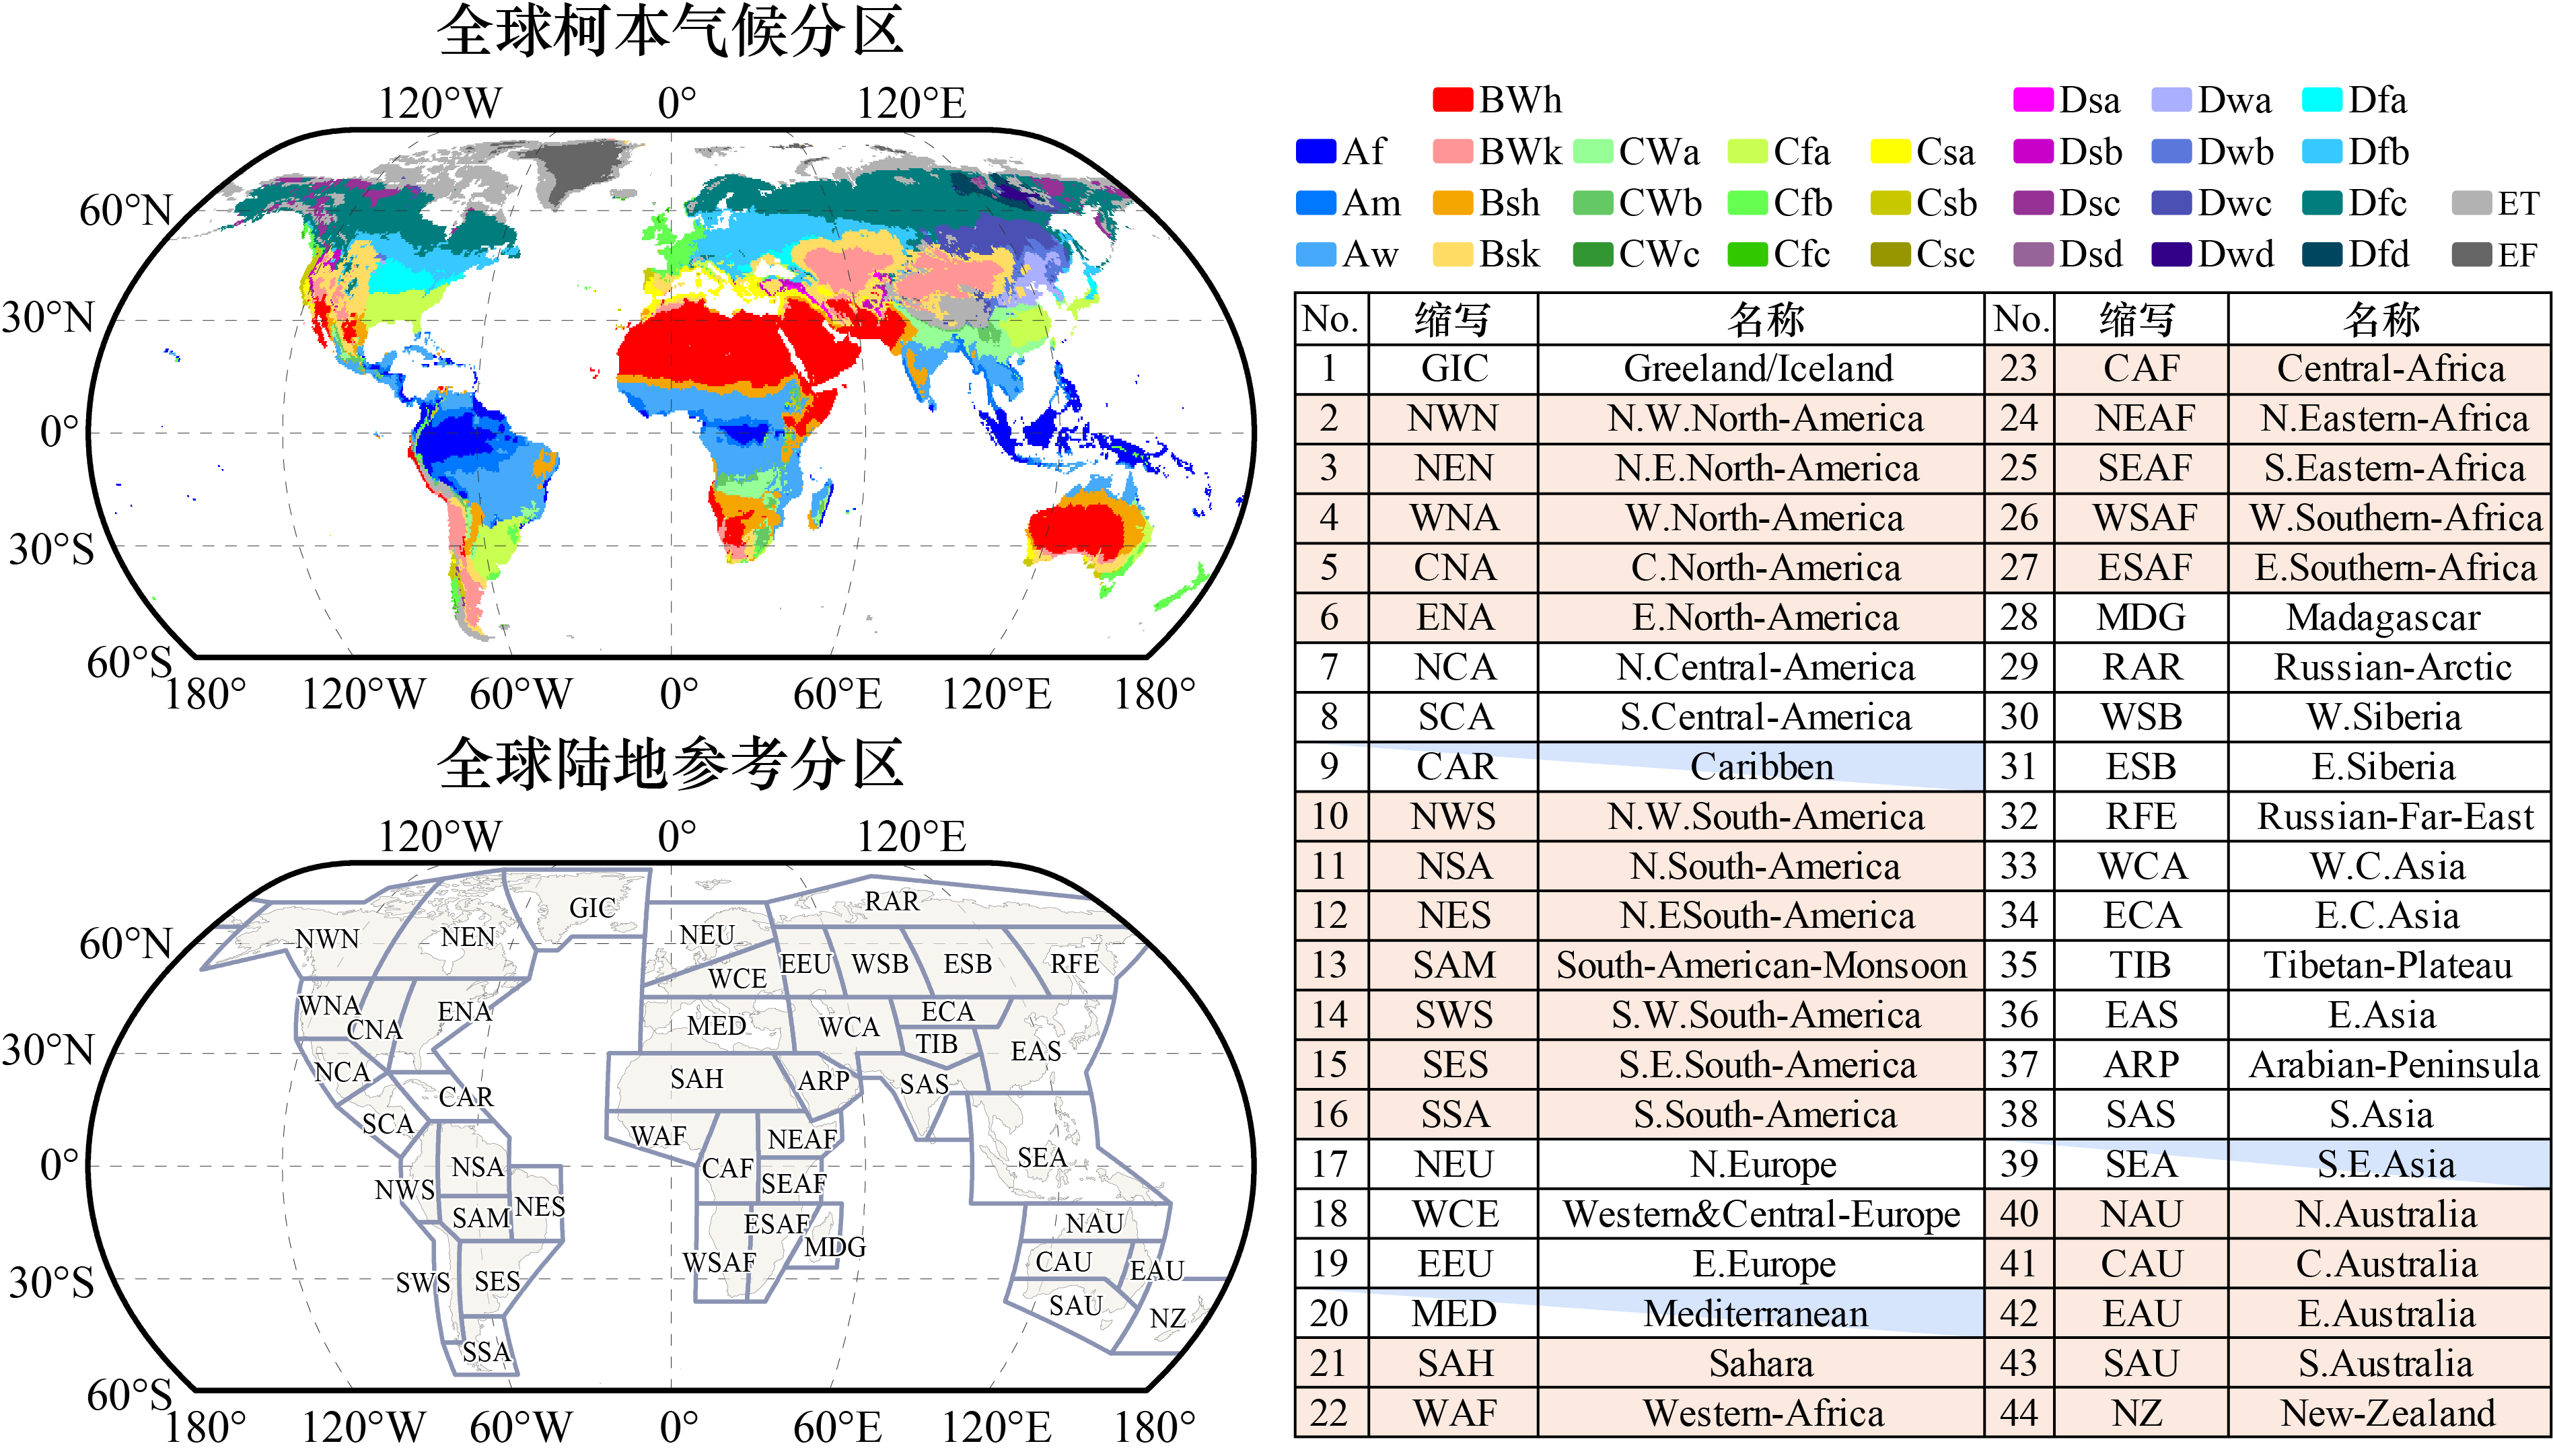
\includegraphics[width=0.9\textwidth]{figures/chap2/Global_Region.jpg}
	\bicaption{全球陆地分区数据}{Köppen and reference region data in global land}\label{fig:Global_Region_Data}
\end{figure}

\clearpage
\chapter{全球陆地关键水循环要素演变格局及多元驱动因子分析}
\label{chap:runoff_trend}

\section{概述}

\section{研究方法}

\subsection{时间序列趋势分析方法}

\subsubsection{线性趋势分析方法}

研究采用基于最小二乘的一元线性回归方法对时间序列进行拟合,得到线性变化的斜率和截距,以此来描述时间序列的变化趋势。同时采用Mann-Kendall非参数趋势检验方法对序列线性变化的显著性进行检验。\par
以时间为自变量,时间序列的观测值为因变量,线性回归模型可以表示为:

\begin{equation}
	slope=\frac{n\times\sum_{t=1}^n\left(t\times Y_t\right)-\sum_{t=1}^nt\times\sum_{t=1}^nY_t}{n\times\sum_{t=1}^nt^2-\left(\sum_{t=1}^nt\right)^2}
\end{equation}

% \subsubsection{非参数趋势检验方法}

\subsubsection{线性-非线性趋势识别算法}

Jamali等\cite{jamaliAutomatedMappingVegetation2014}

\subsection{水文气候序列断点检测算法}

研究采用BFAST算法(Breaks For Additive Seasonal and Trend)对水文气候序列进行断点检测。BFAST是一种基于序列加法分解的断点检测方法,最初被提出用于处理NDVI数据\cite{verbesseltDetectingTrendSeasonal2010,verbesseltPhenologicalChangeDetection2010},但是可被扩展用于各种具有周期特征时间序列,被广泛应用于水文、气象等领域的分析\cite{liTrendSeasonalityAbrupt2022, jiangIdentifyingTrendShifts2022, bernardinoGlobalscaleCharacterizationTurning2020}。算法首先基于STL算法(Seasonal and Trend decomposition using Loess)对时间序列进行分解,得到趋势项、季节项和剩余项三个部分:

\begin{equation}
	Y_t = T_t + S_t + r_t, \qquad  t=1,2,...,n
\end{equation}

式中$Y_t$为时间序列,$T_t$为趋势项,$S_t$为季节项,$r_t$为剩余项,即时间序列中的除了趋势和季节之外的部分。BFAST算法利用基于普通最小二乘(OLS)残差的MOving SUM(MOSUM)检验来确定分解序列中是否存在断点,如果存在,则使用贝叶斯信息准则(BIC)来确定断点的位置和数量,并且分别使用线性函数和三次谐波函数对趋势项和季节项进行分段拟合。假定在趋势项$T_t$中检测出了m个断点$t_1, t_2, ..., t_m$,定义$t_0$=0,$t_{m+1}$=n,在趋势项$S_t$中检测出p个断点$\tau_1, \tau_2, ..., \tau_p$,定义$\tau_0$=0,$\tau_{p+1}$=n,则趋势项和季节项分别被分段拟合为:

\begin{equation}
	\widehat{T_{i,t}}  = \alpha_i + \beta_i t \qquad   \left(t_{i-1}<t\leq t_i, t=1,2,...,m+1 \right)
\end{equation}

\begin{equation}
\begin{aligned}
	\widehat{S_{j,t}}  & = \sum_{h=1}^{k} [\gamma_{j,h} \sin (\frac{2\pi ht}{f} + \mu_h) + \delta_{j,h} \cos (\frac{2\pi ht}{f} + \nu_h)] \\ &  \left(\tau_{j-1}<t\leq \tau_j, j=1,2,...,p+1 \right)
\end{aligned}
\end{equation}

其中$i$,$j$为趋势项和周期项中突变点所在位置,$\alpha_i$,$\beta_i$分别为线性模型的拟合斜率和截距,$\gamma_{j,h}$,$\delta_{j,h}$分别为谐波函数中正弦项和余弦项的振幅参数,$\mu_h$,$\nu_h$为对应项的相位参数,$k$为谐波函数的阶数,在BFAST算法中设置为3。$f$为数据周期频率,如对于月尺度数据,$f$=12。\par
对分段拟合后的结果进行求和,形成新的模拟序列,之后再次进行分解与断点检测步骤,不断迭代更新序列中断点可能发生的事件和显著性,直到最终确定分解结果和鲁棒的断点位置。算法的流程如图\ref{fig:BFAST_intro}所示。\par

\begin{figure}[H]
	\centering
	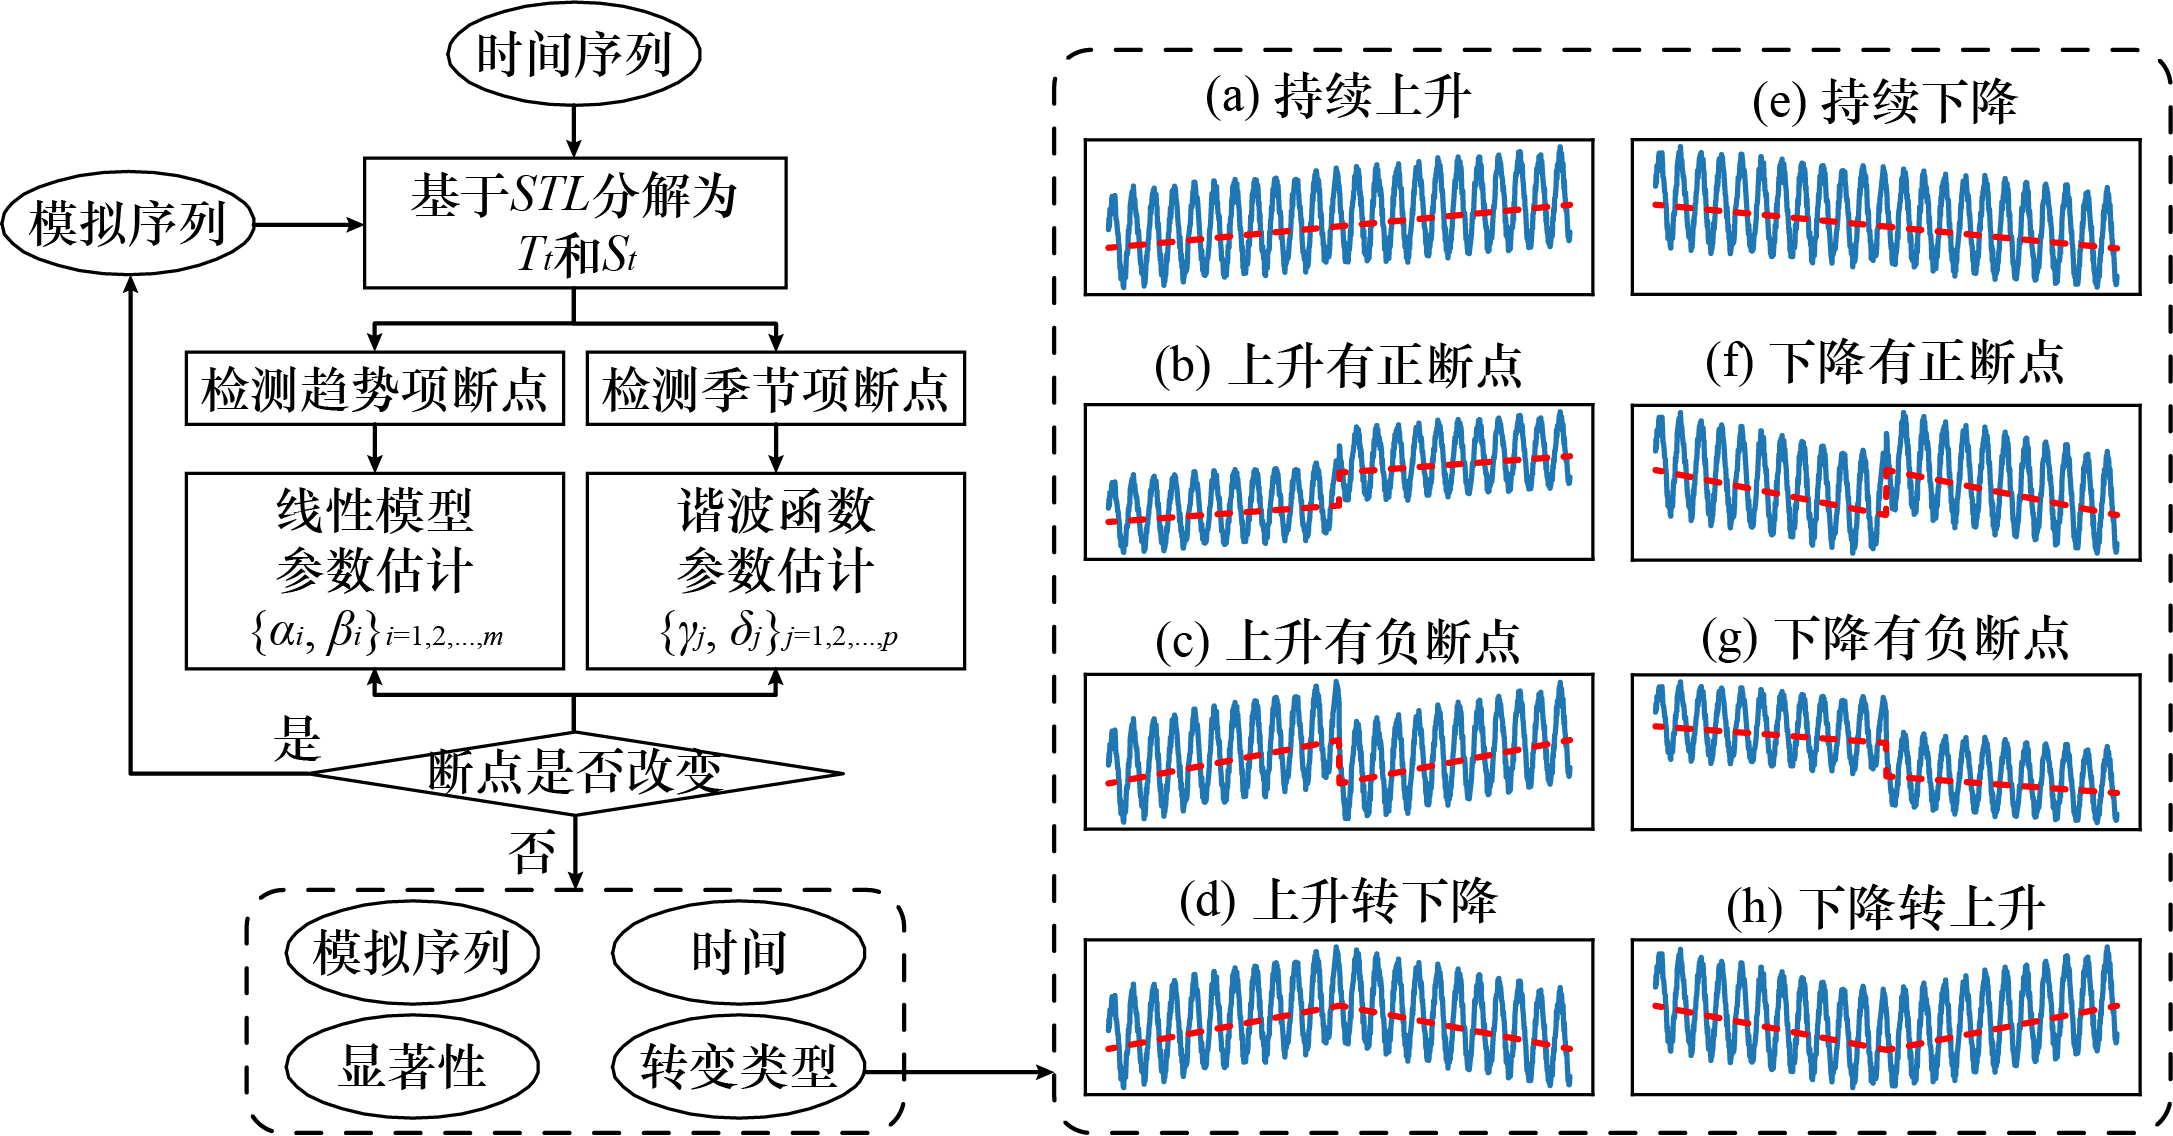
\includegraphics[width=0.9\textwidth]{figures/chap3/0_BFAST_Intro.jpg}
	\bicaption{BFAST算法流程图}{Flowchart of BFAST breakpoint detection algorithm}\label{fig:BFAST_intro}
\end{figure}

本研究使用由R语言开发的“bfast”程序包,逐站点对水文气候序列进行断点检测。程序包中,“bfast”和“bfast01”函数分别对应算法的泛化模式和变化检测模式。其中泛化模式能够指定断点数量,并基于上面介绍的分解拟合算法对原始时间序列进行模拟,变化检测模式是检测完整时间序列中是否存在一个最显著的断点,并提取断点的起始时间、变化类型、显著性等详细信息\cite{JiangPing19822015NianZhongGuoZhiBeiFuGaiBianHuaJiQiDuiQiHouBianHuaDeMinGanXingFenXi2022}。根据断点前后序列趋势变化的方向及显著性差异,“bfast01”函数将趋势变化分为8种类型,分别是:持续上升、持续下降、持续上升并有正向断点、持续上升并有负向断点、持续下降并有正向断点、持续下降并有负向断点、上升转下降、下降转上升,以提供对时间序列变化断点更详细的了解。\par

\subsection{基于数据驱动的数据缺失值插补方法}

由于BFAST断点检测算法对时间序列中缺失值敏感,为了保证算法的准确性与可执行性,需要对原始径流序列中的缺失值与无效值进行插补。由于本研究的目的是对实测径流进行分析,因此插补方法需要尽可能保留原始数据的特征,同时尽量减少插补过程中引入的不确定性。在本研究中,采用了基于数据驱动的插补方法,即基于径流序列的历史数据和其他气象要素的数据,通过数据间的相关性来插补缺失值。基于数据驱动的插补方法的基本思想是通过已有数据的特征来推断缺失数据的值,根据非缺失值时间段内的气候数据与径流观测建立联系,训练并评估机器学习模型,利用数据缺失时段的气候数据驱动训练好的模型,对缺失时段的径流进行插补。缺失径流数据插补的基本框架如图\ref{fig:Interp_Framework}所示。\par

\begin{figure}[H]
	\centering
	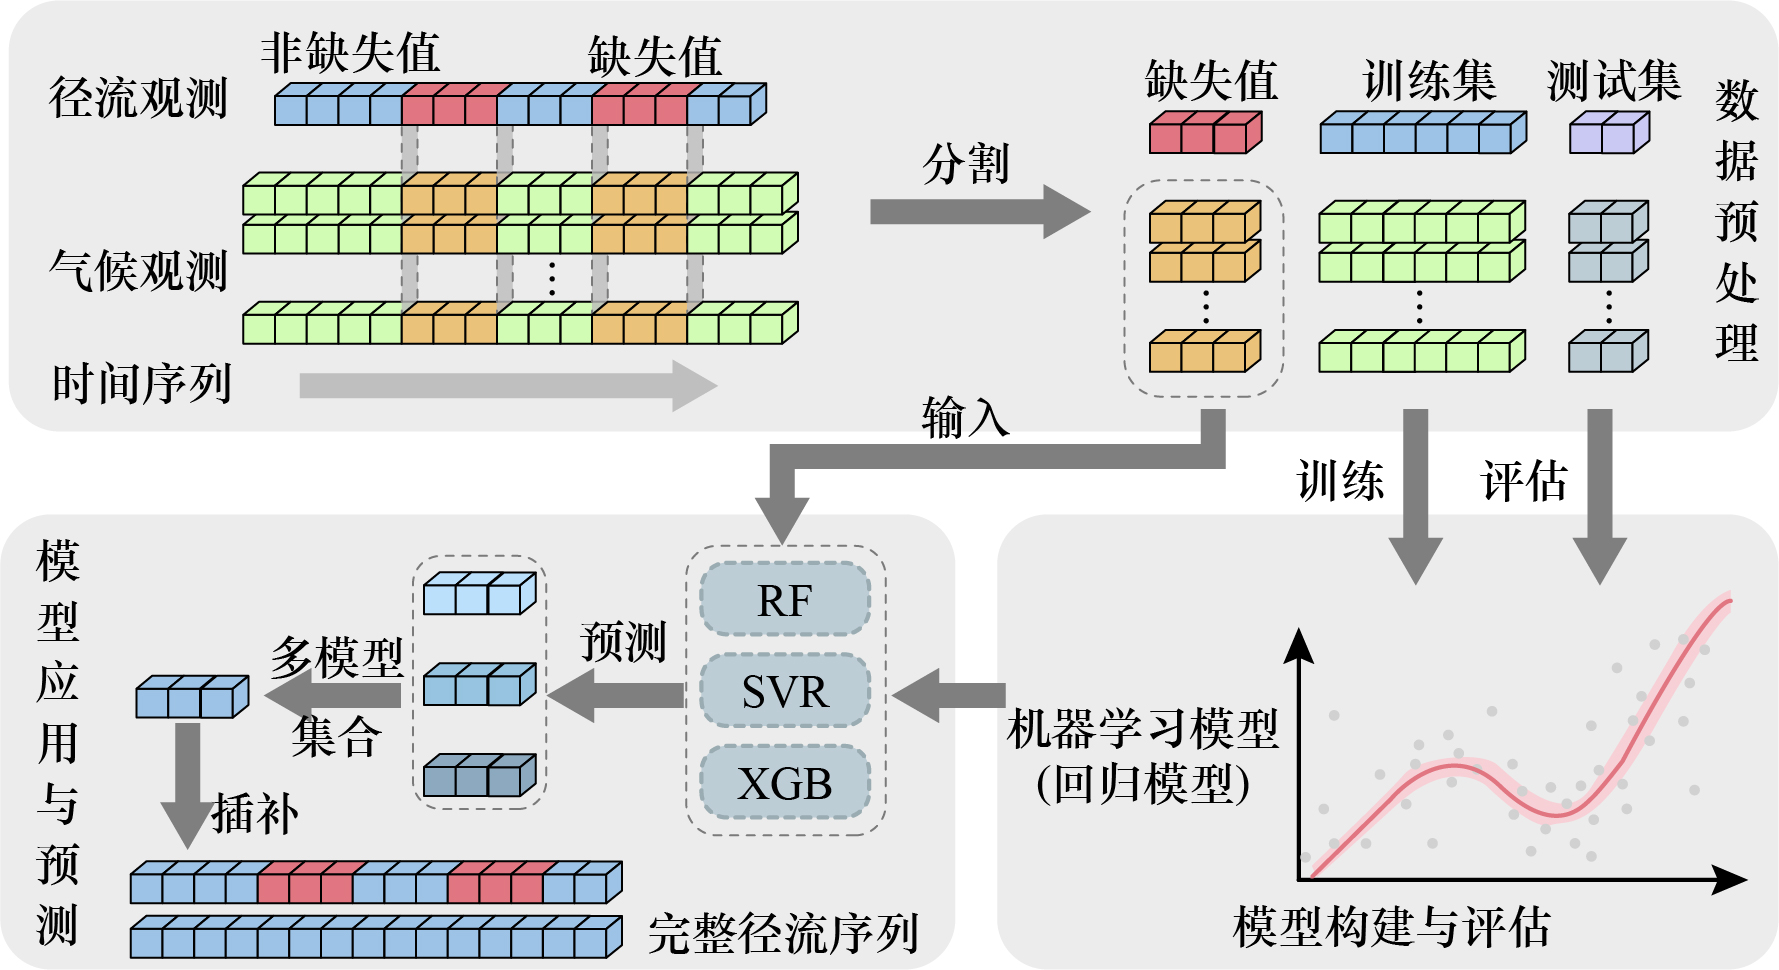
\includegraphics[width=0.85\textwidth]{figures/chap3/0_Interp_Framework.jpg}
	\bicaption{径流缺失数据插补流程图}{Interpolation flowchart of missing runoff data}
	\label{fig:Interp_Framework}
\end{figure}

本研究采用了三种常用的回归类型机器学习算法构建流域气候条件与实测径流之间的关系,分别是支持向量机回归(Support Vector Machine Regression,SVR)、随机森林(Random Forest,RF)和极端梯度提升(eXtreme Gradient Boosting,XGBoost)。这三种算法在机器学习领域中被广泛应用于回归问题,具有较好的拟合能力和泛化能力。在本研究中,对于每个流域,将径流数据作为目标变量,其他气象要素(降水、潜在蒸散发、最高气温、最低气温和平均气温)的数据作为特征变量,构建回归模型。考虑到气候条件对径流的滞后影响,每种气候变量的滞后阶数设置在0-3之间,因此有5(气象要素)×4(滞后时段)共20种特征变量。在模型训练阶段,采用了5折交叉验证的方法,以减少模型过拟合的风险。采用预测结果与实测结果的纳什效率系数(Nash-Sutcliffe Efficiency Coefficient,NSE)、相对误差(Relative Error,RE)和相关系数(Correlation Coefficient,CC),均方根误差(Root Mean Square Error,RMSE)作为评价指标,以评估模型的模拟结果与泛化能力。

\begin{equation}
    \label{equ:NSE}
	NSE=1-\frac{\sum_{t=1}^{n}\left(Q o_{i}-Q s_{i}\right)^{2}}{\sum_{t=1}^{n}\left(Q o_{i}-\overline{Q o}\right)^{2}}
\end{equation}

\begin{equation}
    \label{equ:RE}
	RE=\frac{\overline{Q_s}-\overline{Q_o}}{\overline{Q_o}}
\end{equation}

\begin{equation}
    \label{equ:CC}
	CC=\frac{\sum_{t=1}^{n}((Q_{o_i}-\overline{Q_o})(Q_{s_i}-\overline{Q_s}))}{\sqrt{\sum_{t=1}^{n}(Q_{o_i}-\overline{Q_o})^2\sum_{t=1}^{n}(Q_{s_i}-\overline{Q_s})^2}} 
\end{equation}

\begin{equation}
    \label{equ:RMSE}
	RMSE=\sqrt{ \sum_{t=1}^{n}\frac{(Q_{s_i}-Q_{o_i})^2}{n} }  
\end{equation}

式中$Q_o$和$Q_s$分别代表了观测值和模拟值,$\overline{Q_o}$和$\overline{Q_s}$分别代表了观测值和模拟值的平均值,$n$为样本数量。\par
在模型应用阶段,利用数据缺失时段的气候数据驱动训练好的模型,预测缺失时段的径流数据。为了减少模型预测结果的不确定性,对于每个流域,采用三种机器学习算法分别进行插补,最终插补结果取三种算法的平均值作为最终插补结果。\par

% \subsection{径流变化归因分析方法}

% \subsubsection{多年尺度径流变化归因分析方法}

% \subsubsection{径流年内变异性归因分析方法}

% \section{全球历史气候要素时空演变格局}

% \subsection{全球气候要素时空变化特征}

% \begin{figure}[H]
% 	\centering
% 	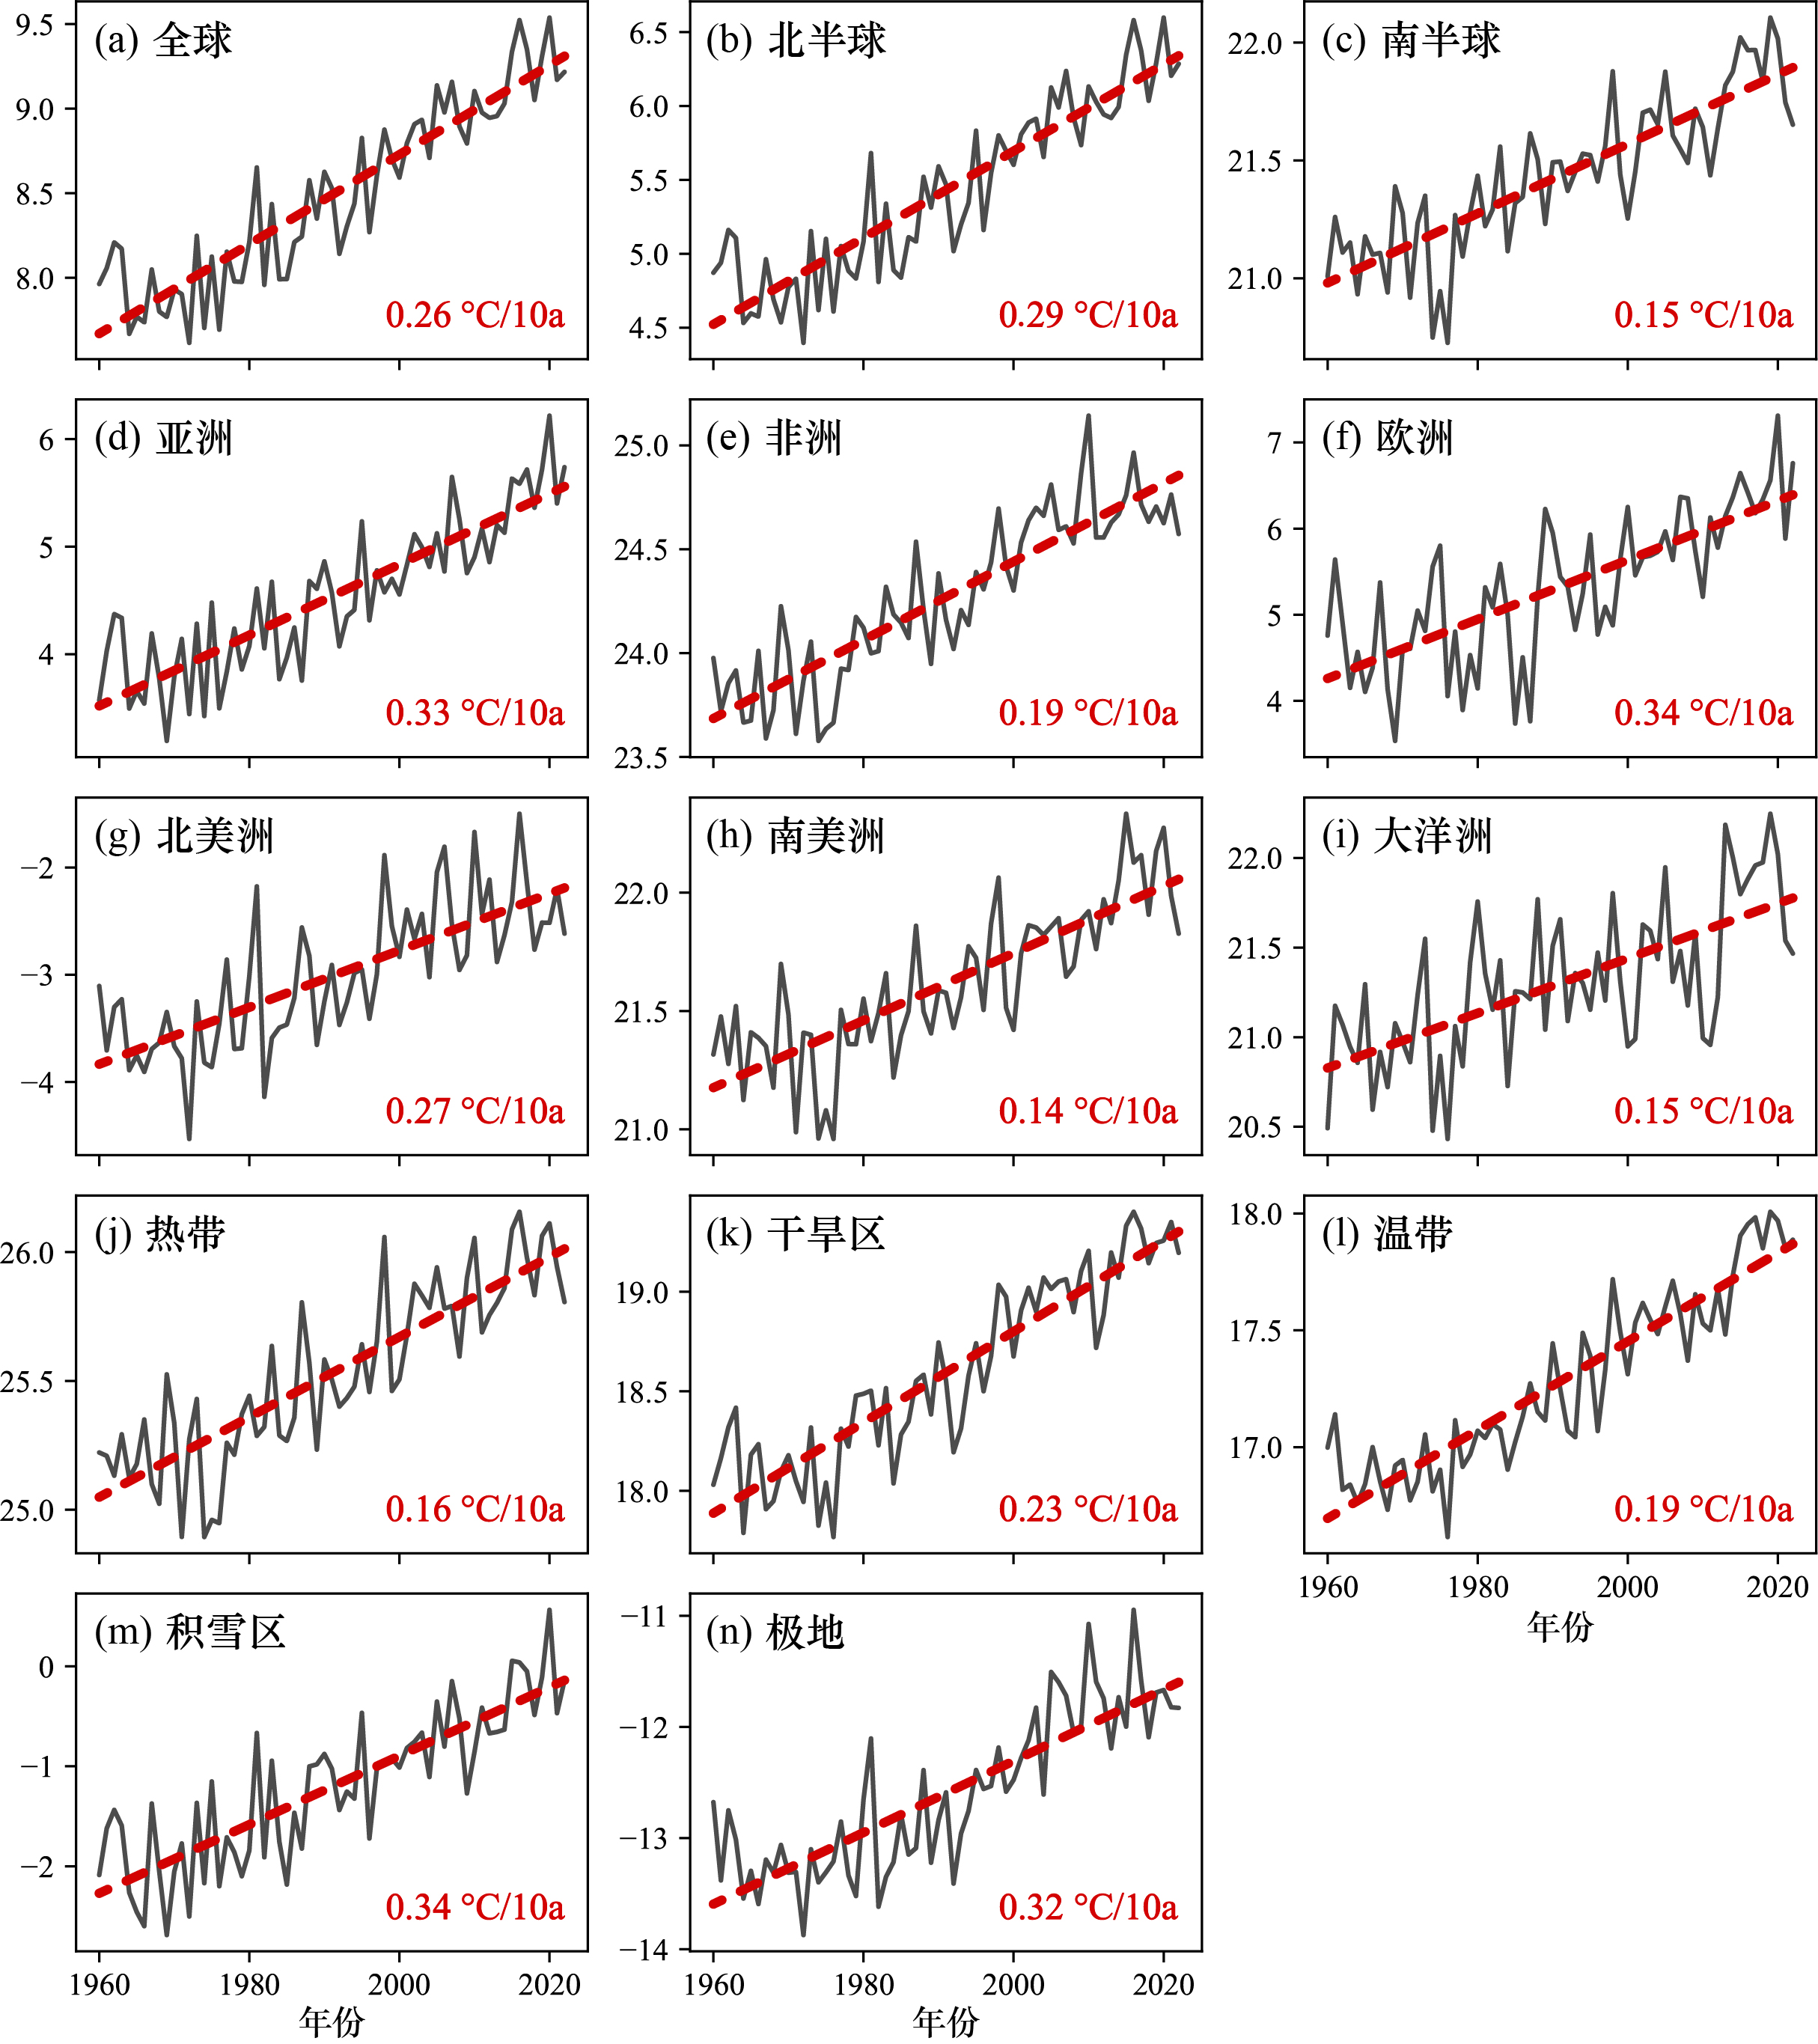
\includegraphics[width=0.85\textwidth]{figures/chap3/1_TEM_Series.jpg}
% 	\bicaption{全球及区域气温序列及变化趋势}{Temperature series and linear trend in global and regional scale}
% 	\label{fig:TEM_Series}
% \end{figure}

% \begin{figure}[H]
% 	\centering
% 	\includegraphics[width=0.85\textwidth]{figures/chap3/1_TT.jpg}
% 	\bicaption{全球年、季尺度气温变化空间格局}{Spatial pattern of annual and seasonal temperature trend}
% 	\label{fig:TEM_Trend_Map}
% \end{figure}

% \begin{figure}[H]
% 	\centering
% 	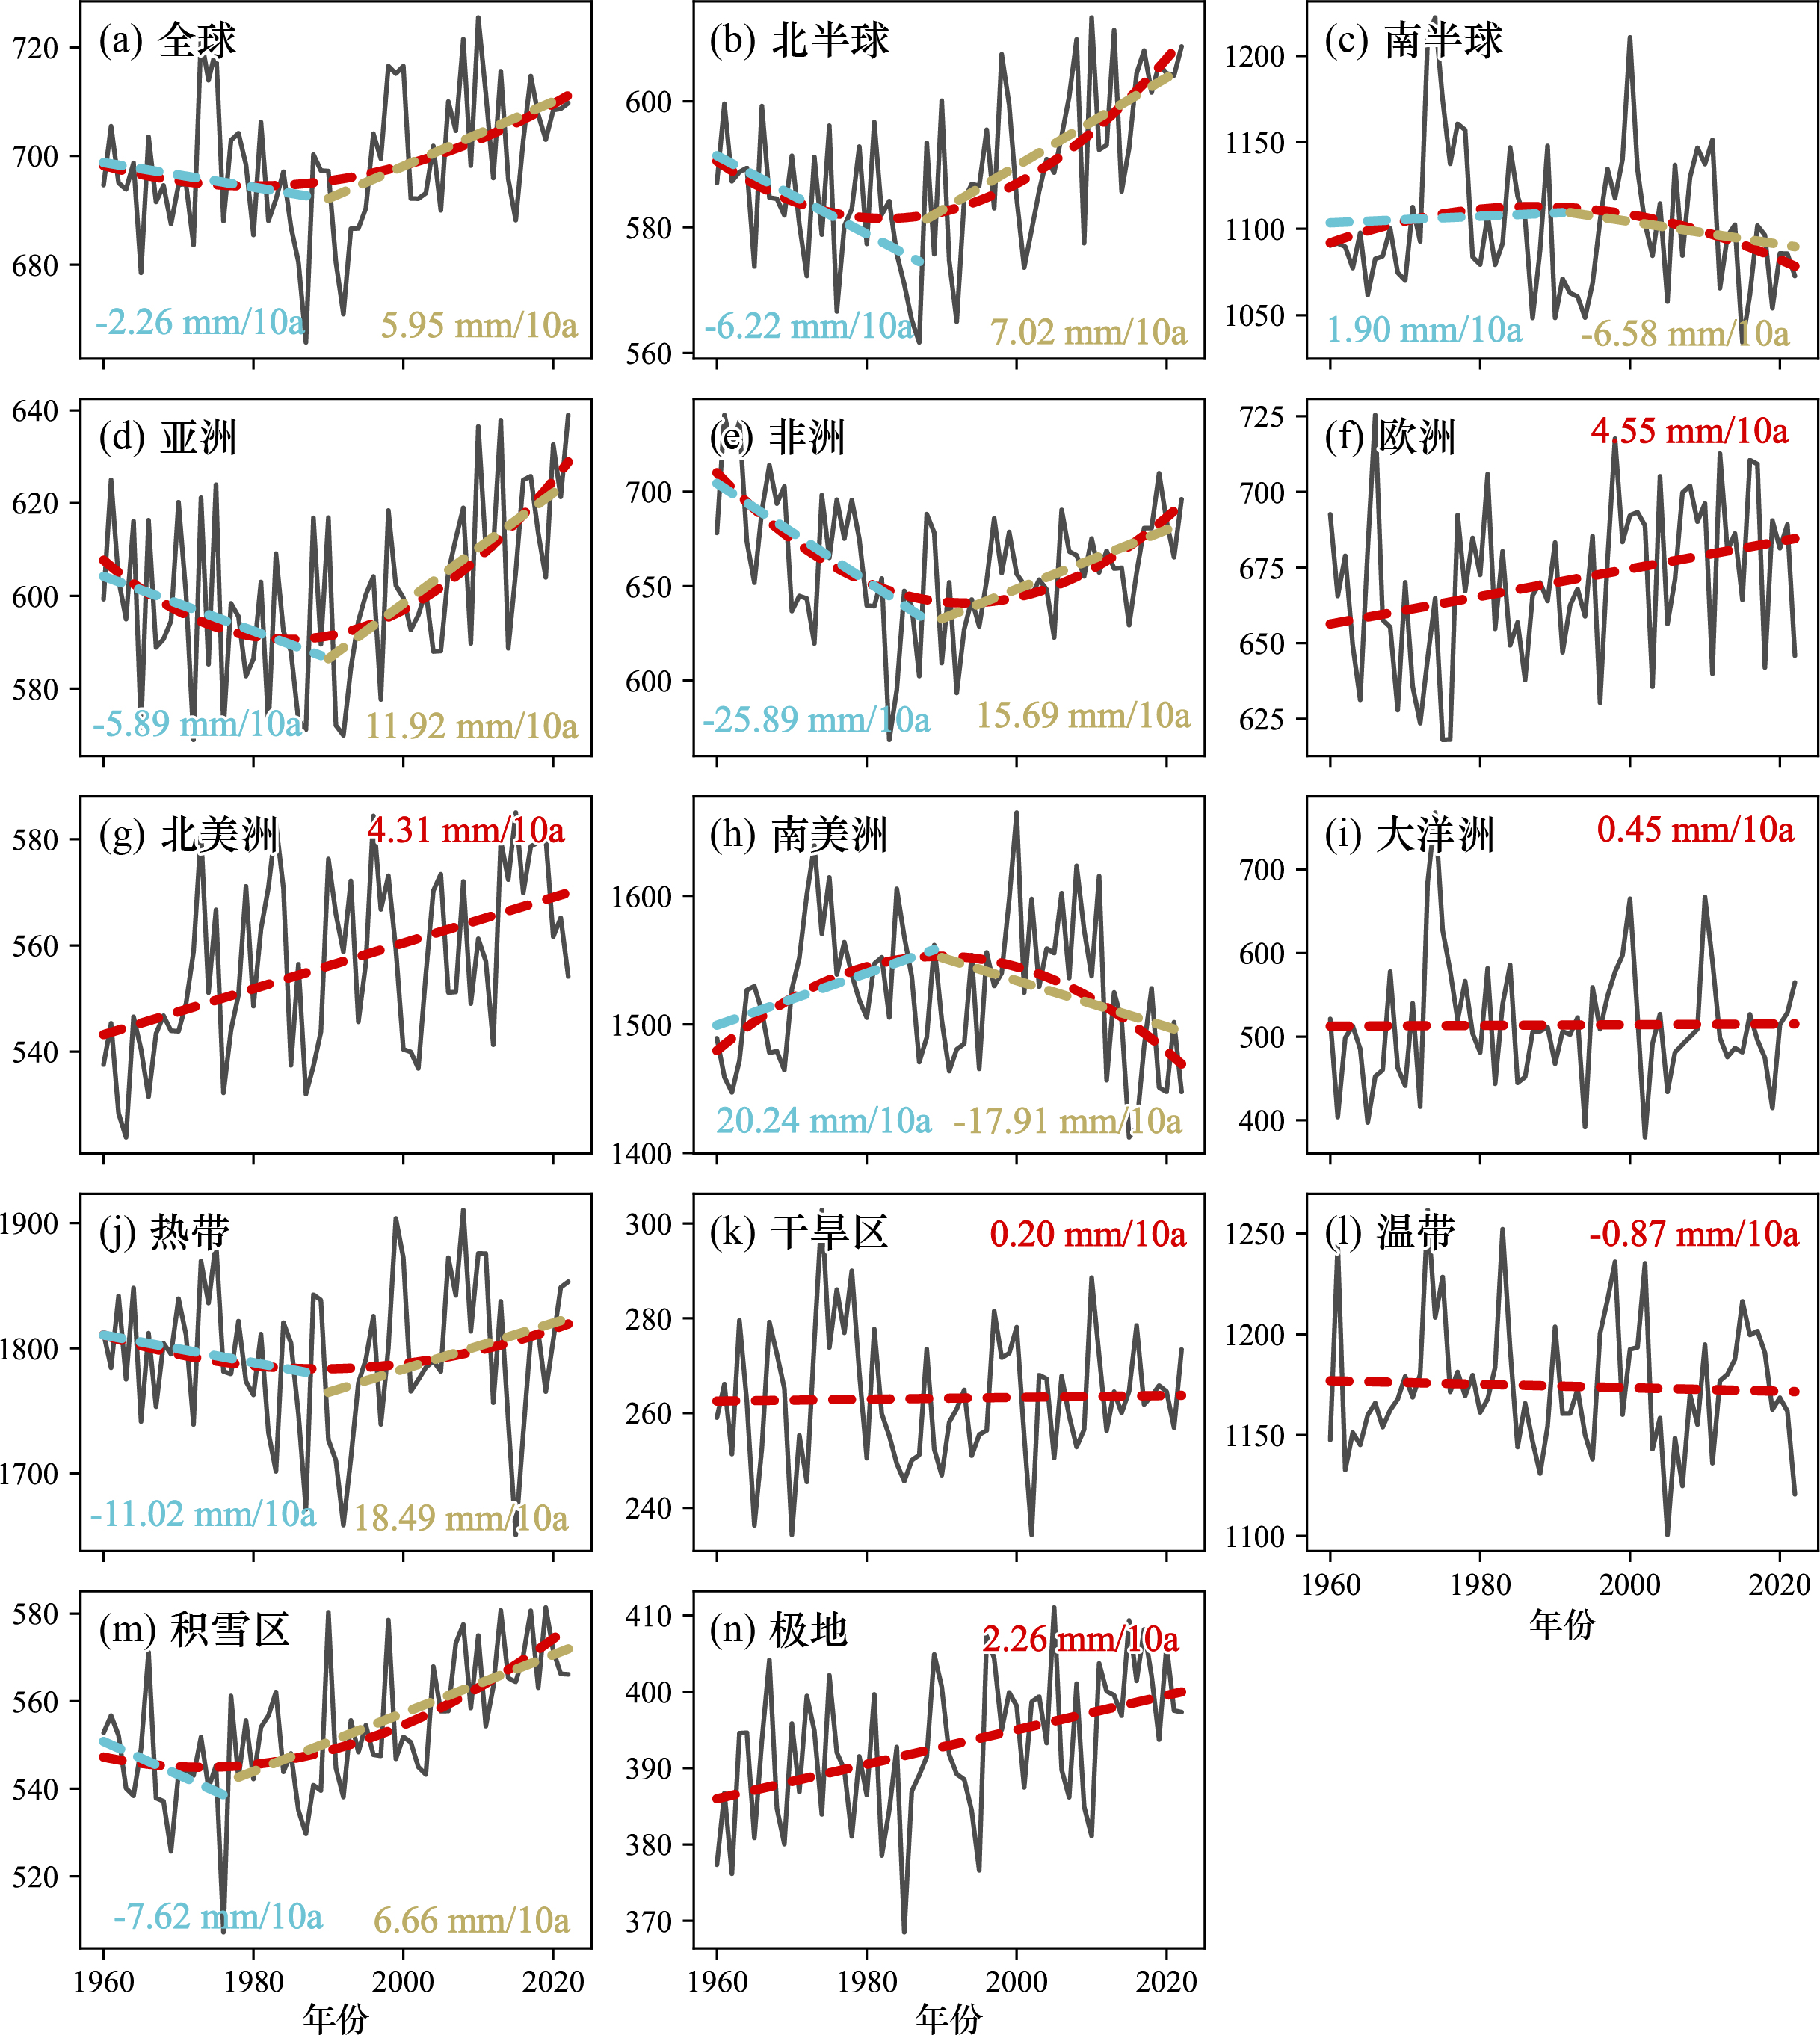
\includegraphics[width=0.85\textwidth]{figures/chap3/1_PRE_Series.jpg}
% 	\bicaption{全球及区域降水序列及变化趋势}{Precipitation series and linear trend in global and regional scale}
% 	\label{fig:PRE_Series}
% \end{figure}

% \begin{figure}[H]
% 	\centering
% 	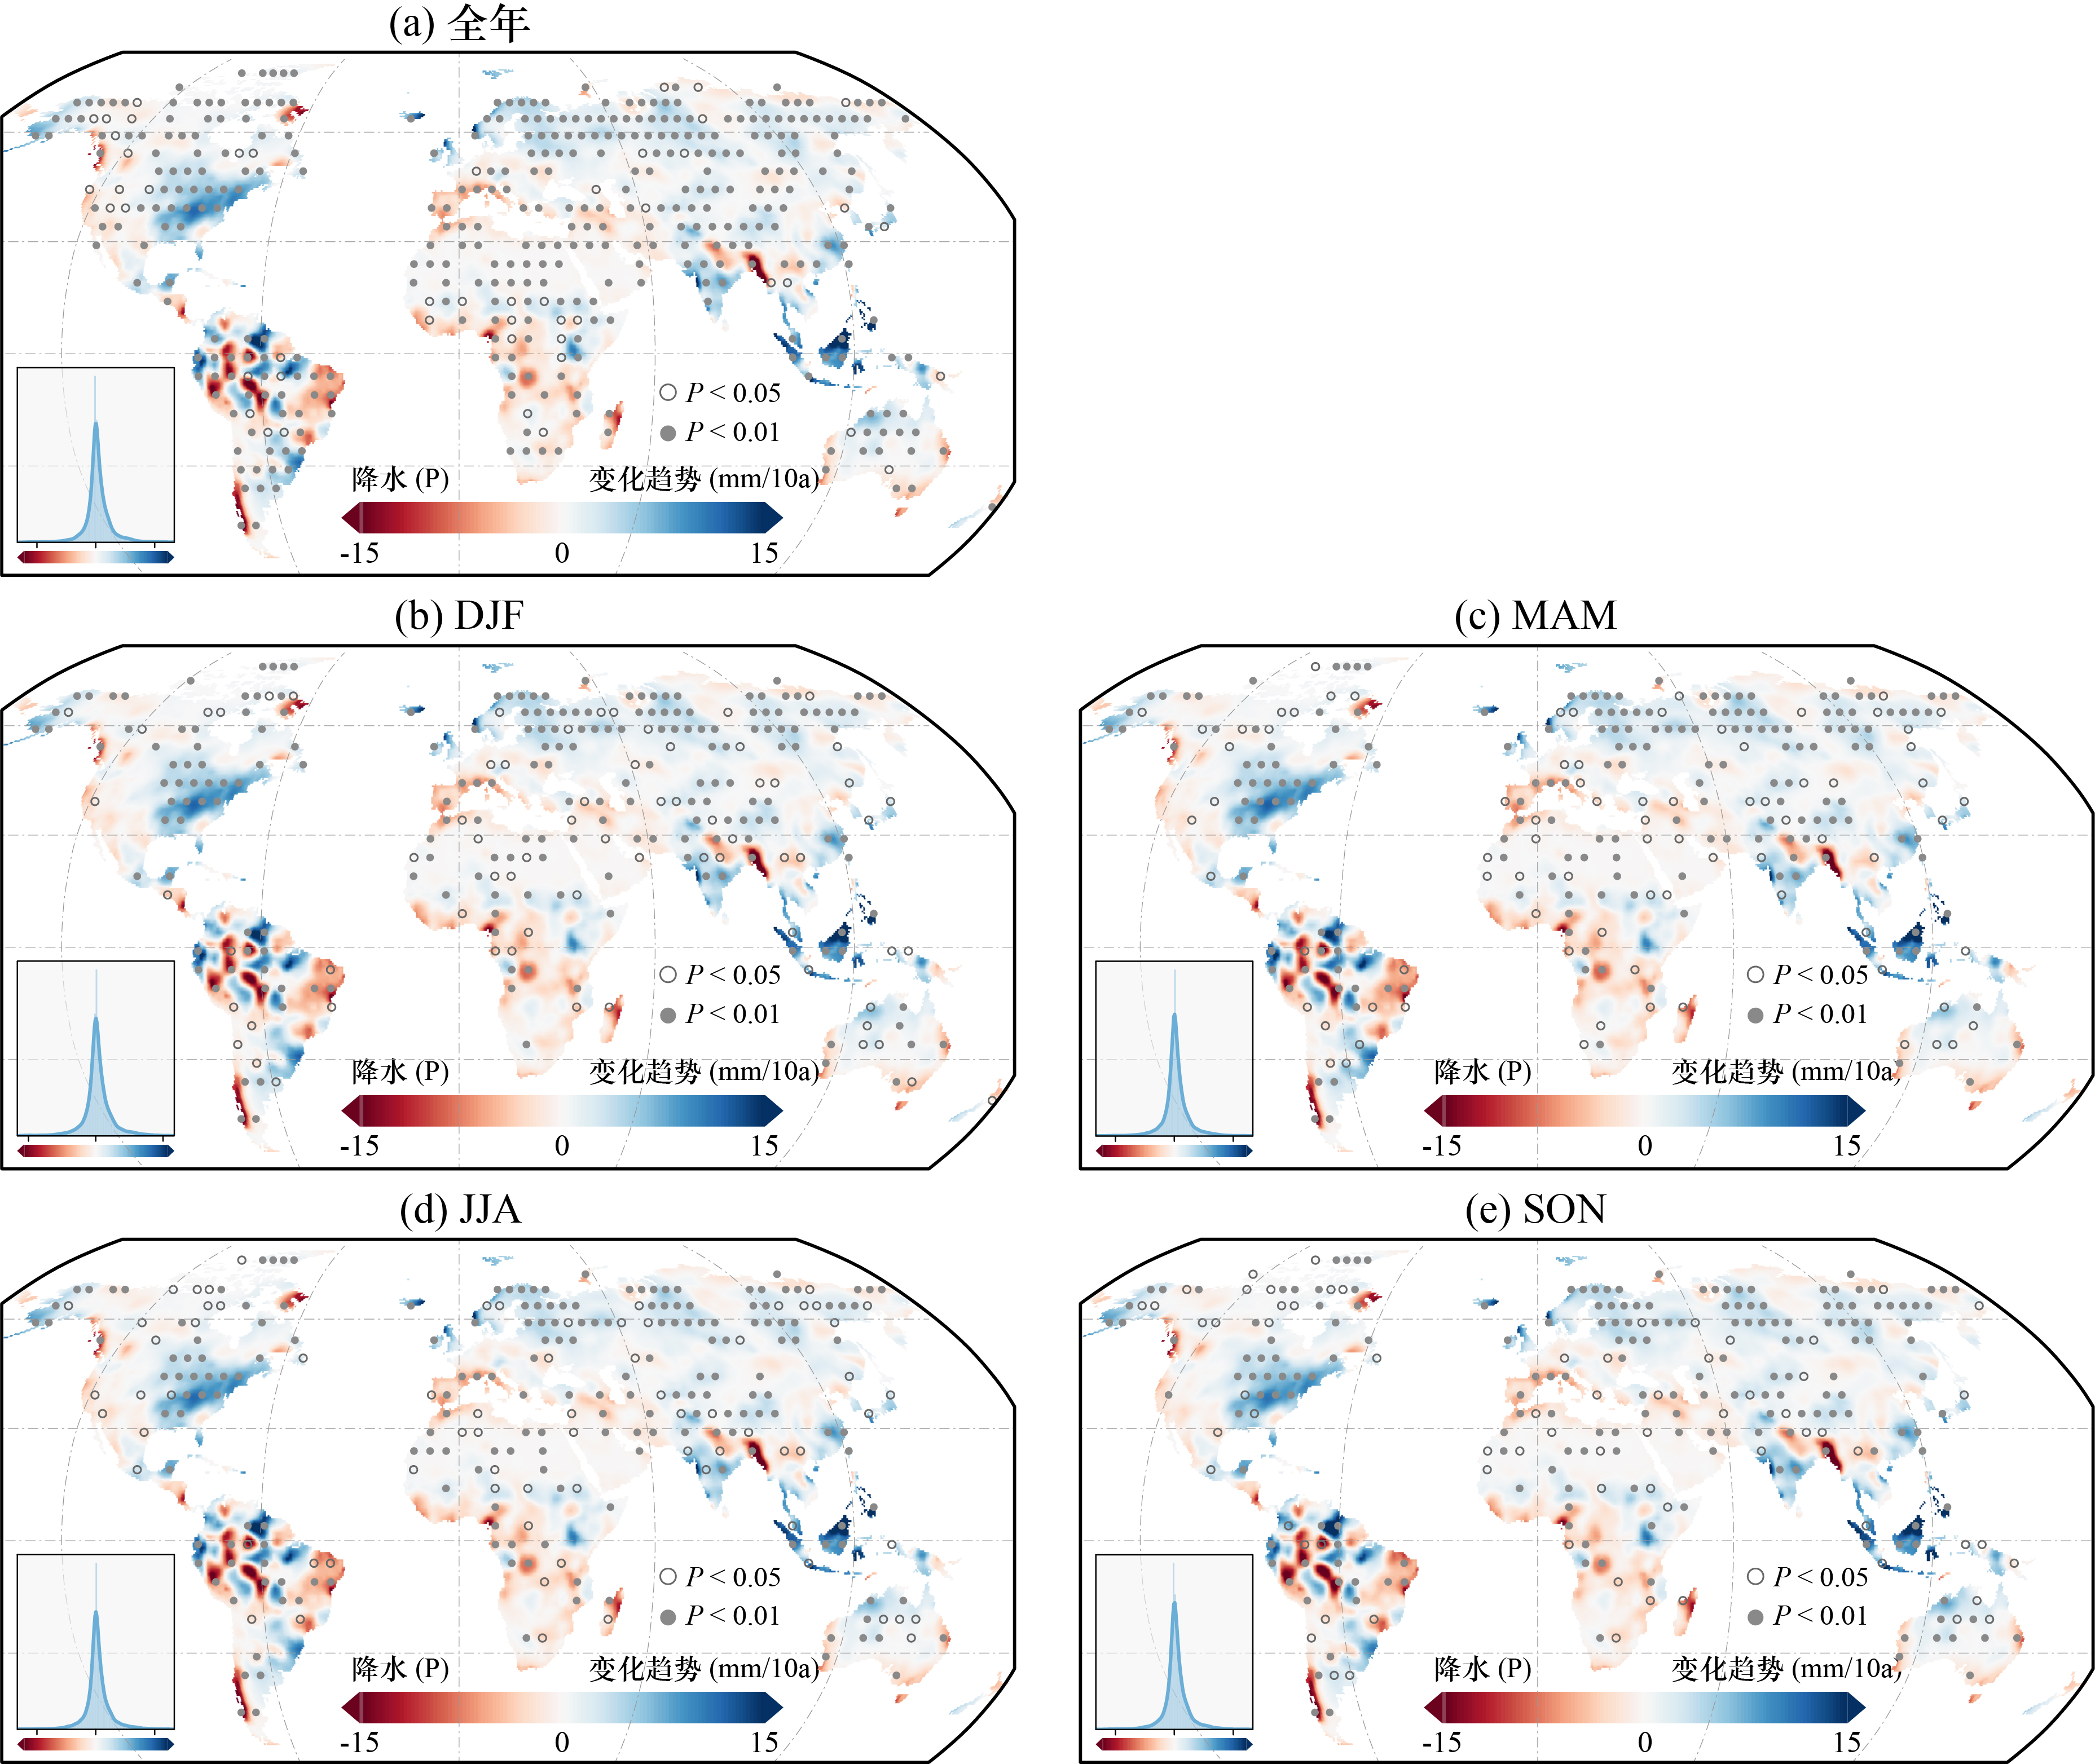
\includegraphics[width=0.85\textwidth]{figures/chap3/1_PT.jpg}
% 	\bicaption{全球年、季尺度降水变化空间格局}{Spatial pattern of annual and seasonal precipitation trend}
% 	\label{fig:PRE_Trend_Map}
% \end{figure}

% \begin{figure}[H]
% 	\centering
% 	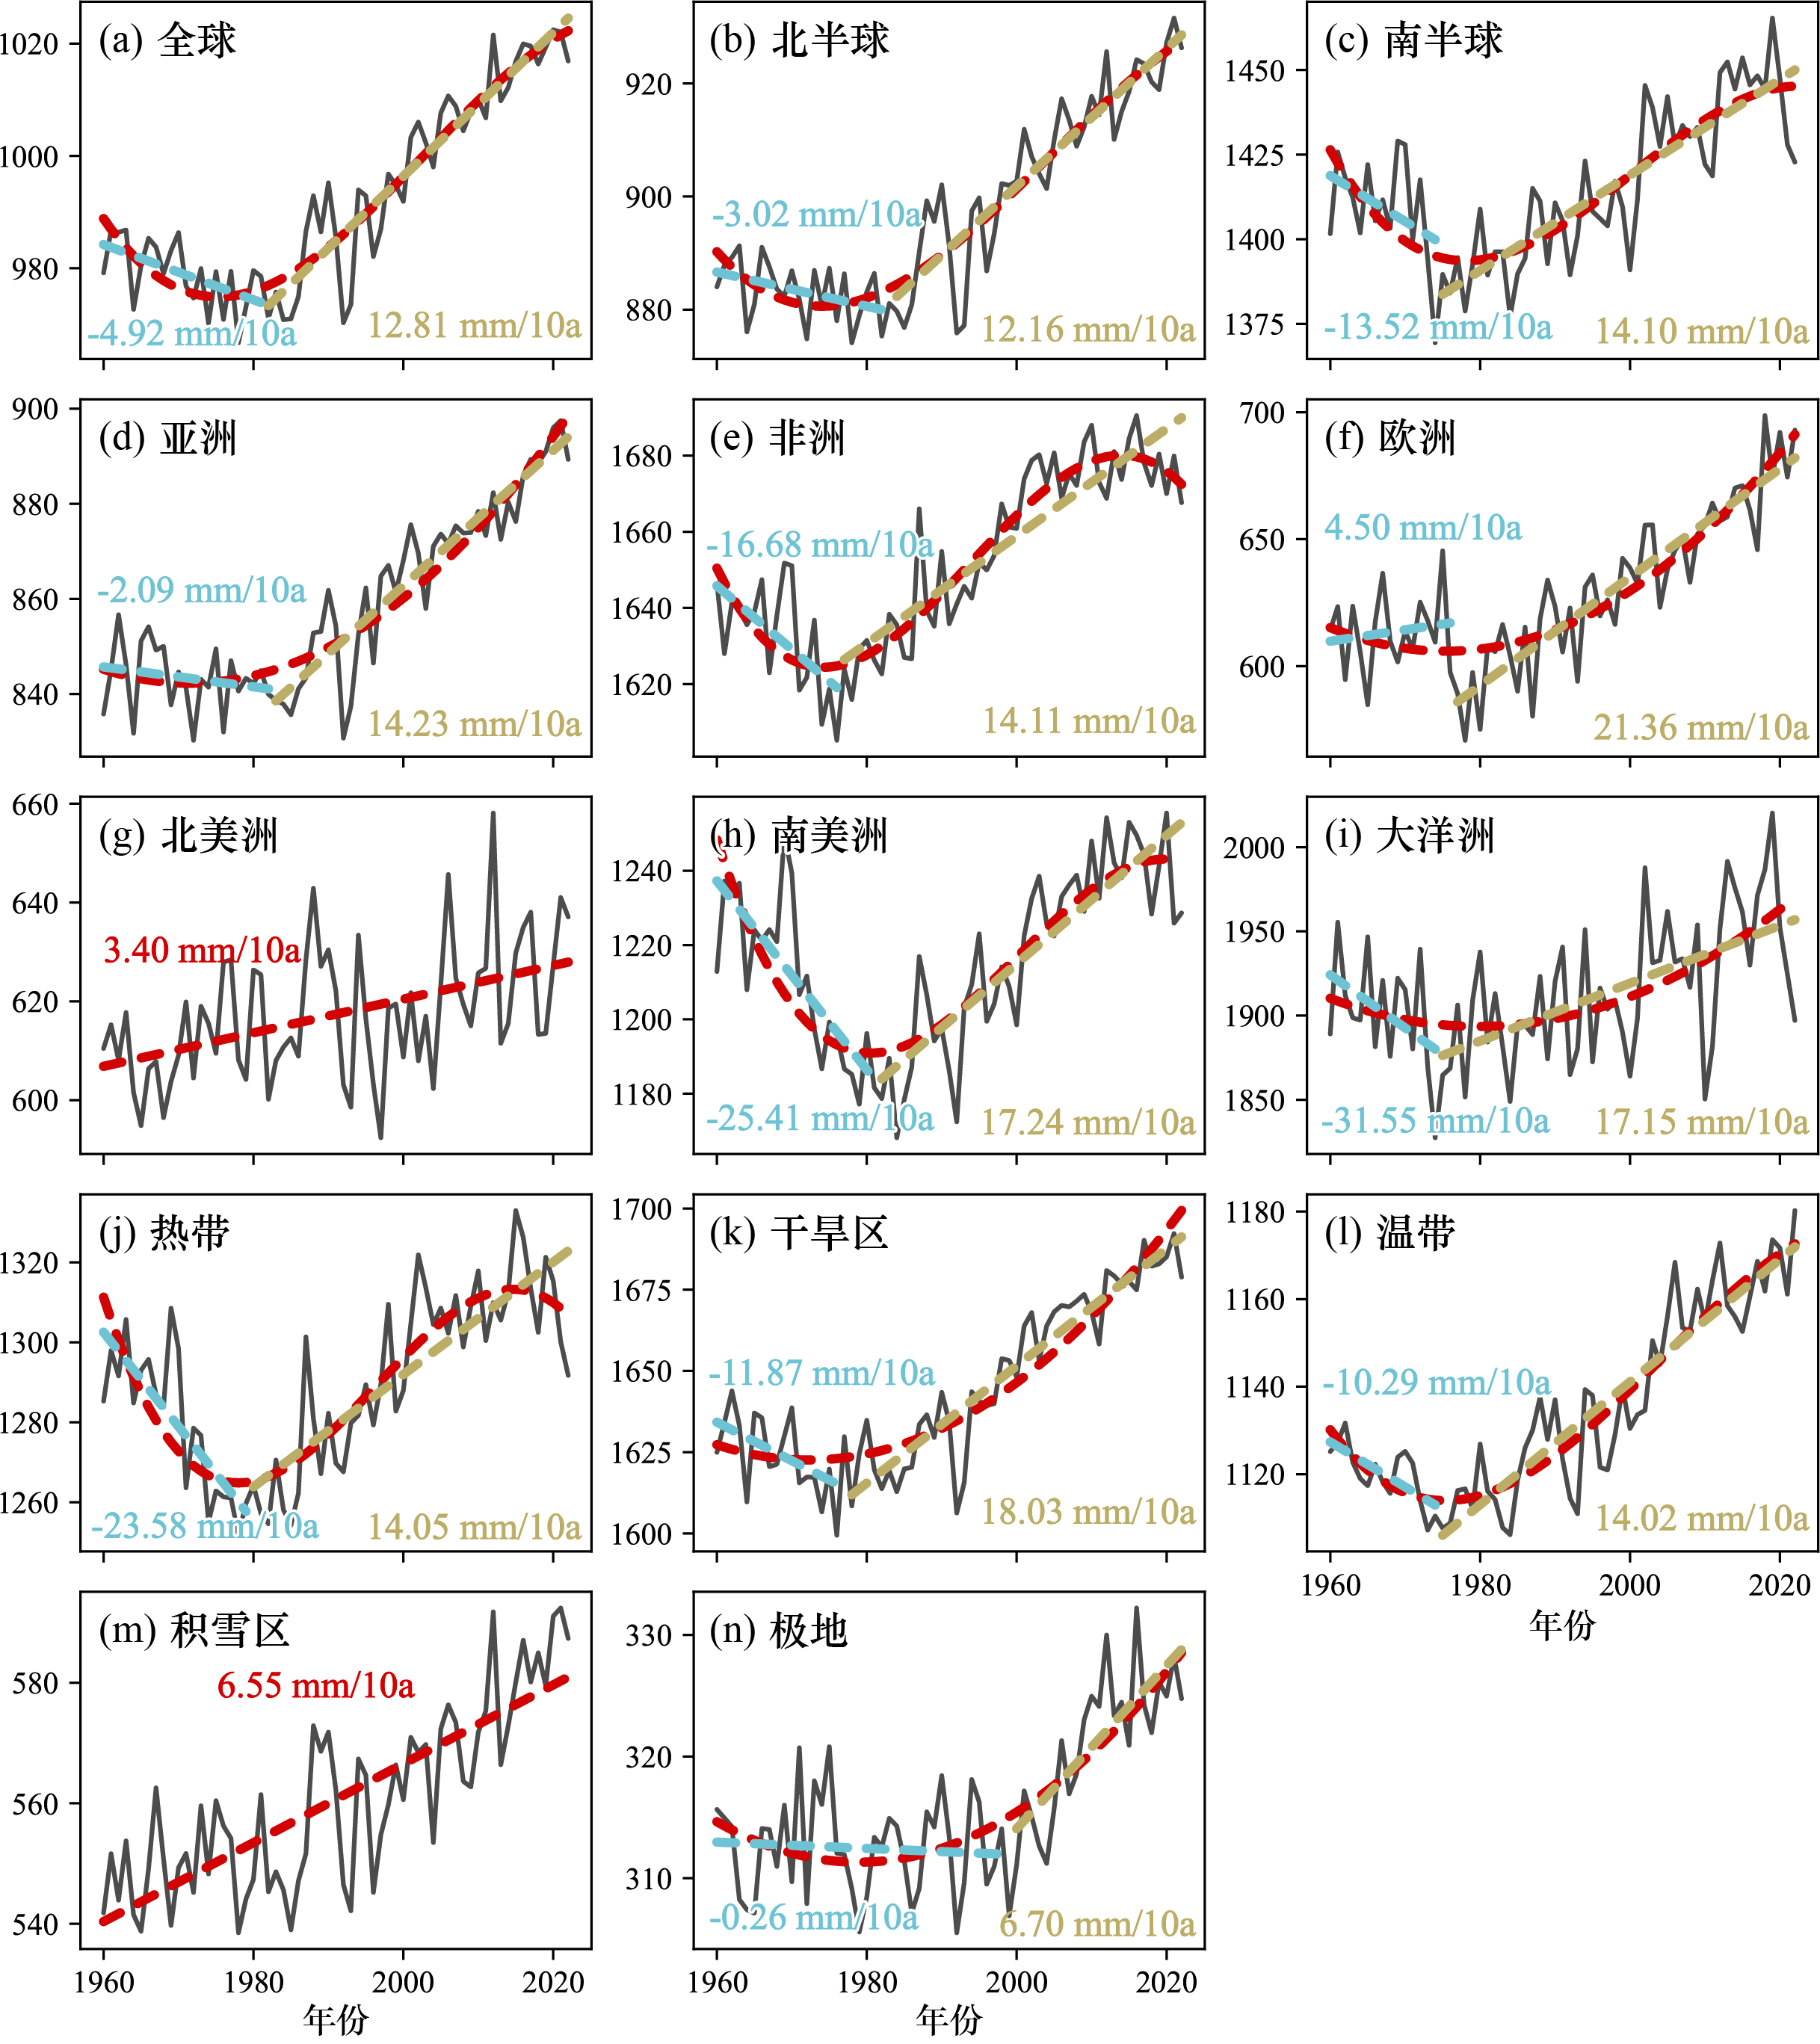
\includegraphics[width=0.85\textwidth]{figures/chap3/1_PET_Series.jpg}
% 	\bicaption{全球及区域潜在蒸散发序列及变化趋势}{Potential evapotranspiration series and linear trend in global and regional scale}
% 	\label{fig:PET_Series}
% \end{figure}

% \begin{figure}[H]
% 	\centering
% 	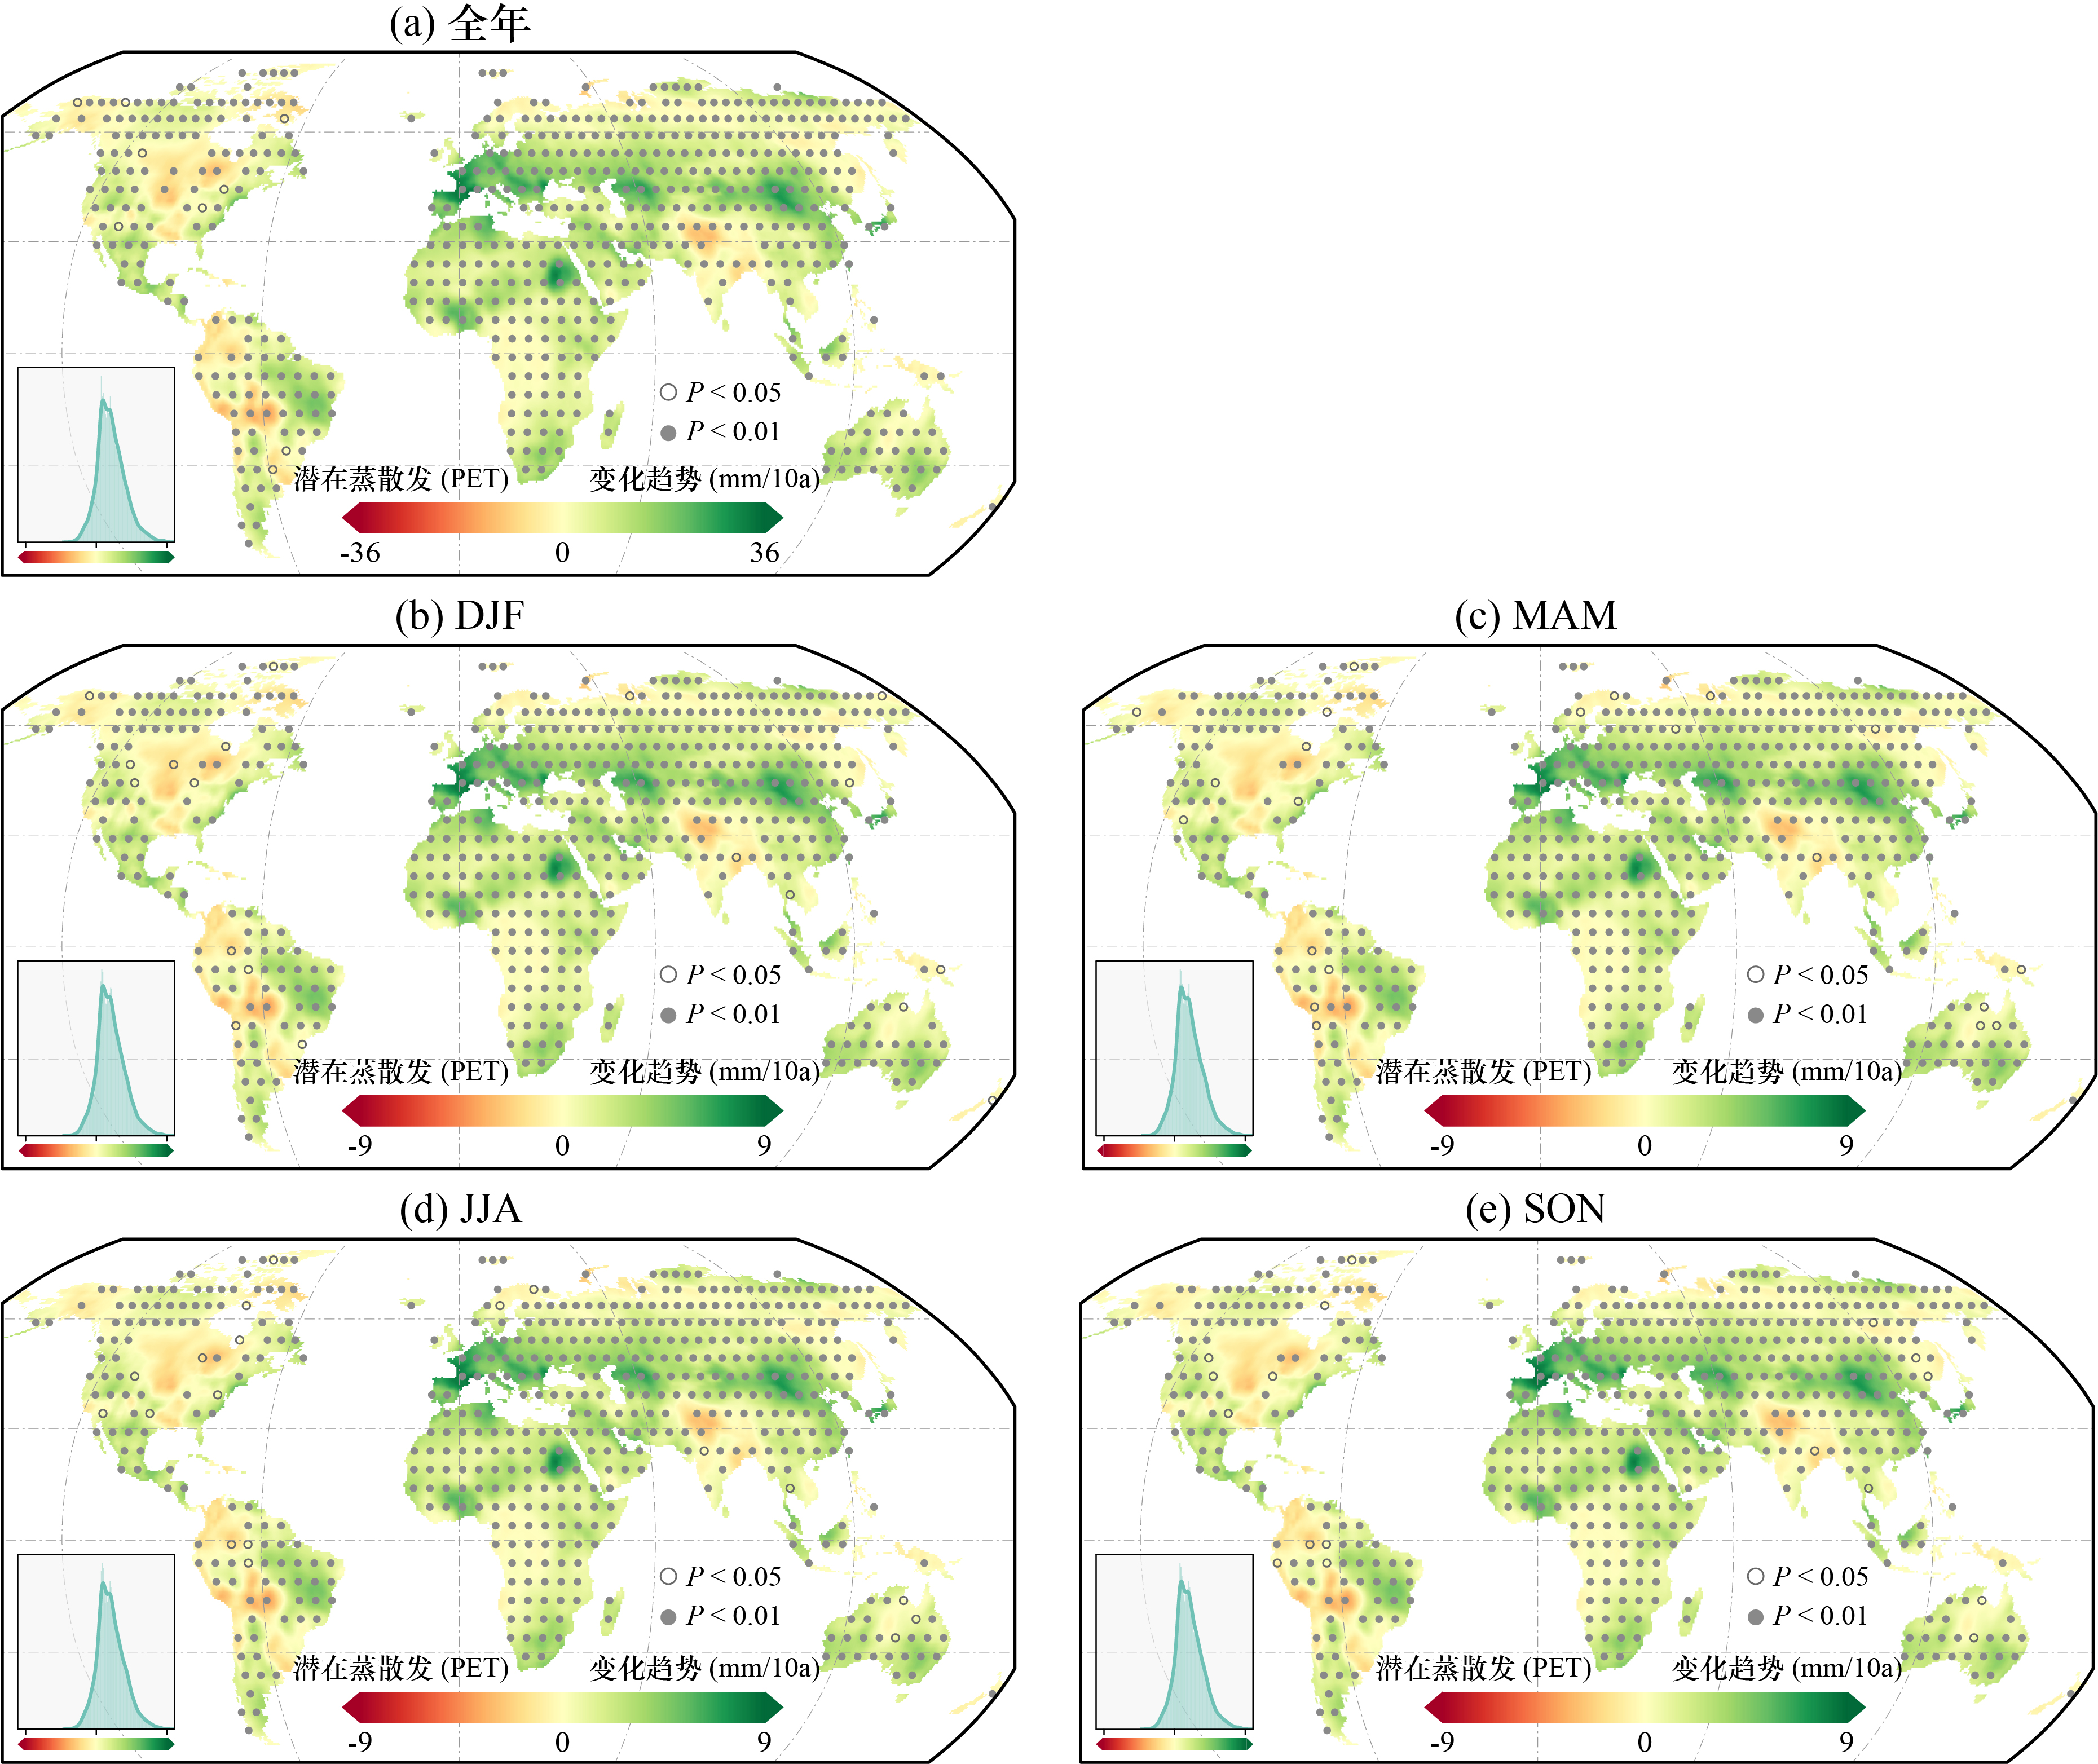
\includegraphics[width=0.85\textwidth]{figures/chap3/1_ET.jpg}
% 	\bicaption{全球年、季尺度潜在蒸散发变化空间格局}{Spatial pattern of annual and seasonal potential evapotranspiration trend}
% 	\label{fig:PET_Trend_Map}
% \end{figure}

% \begin{figure}[H]
% 	\centering
% 	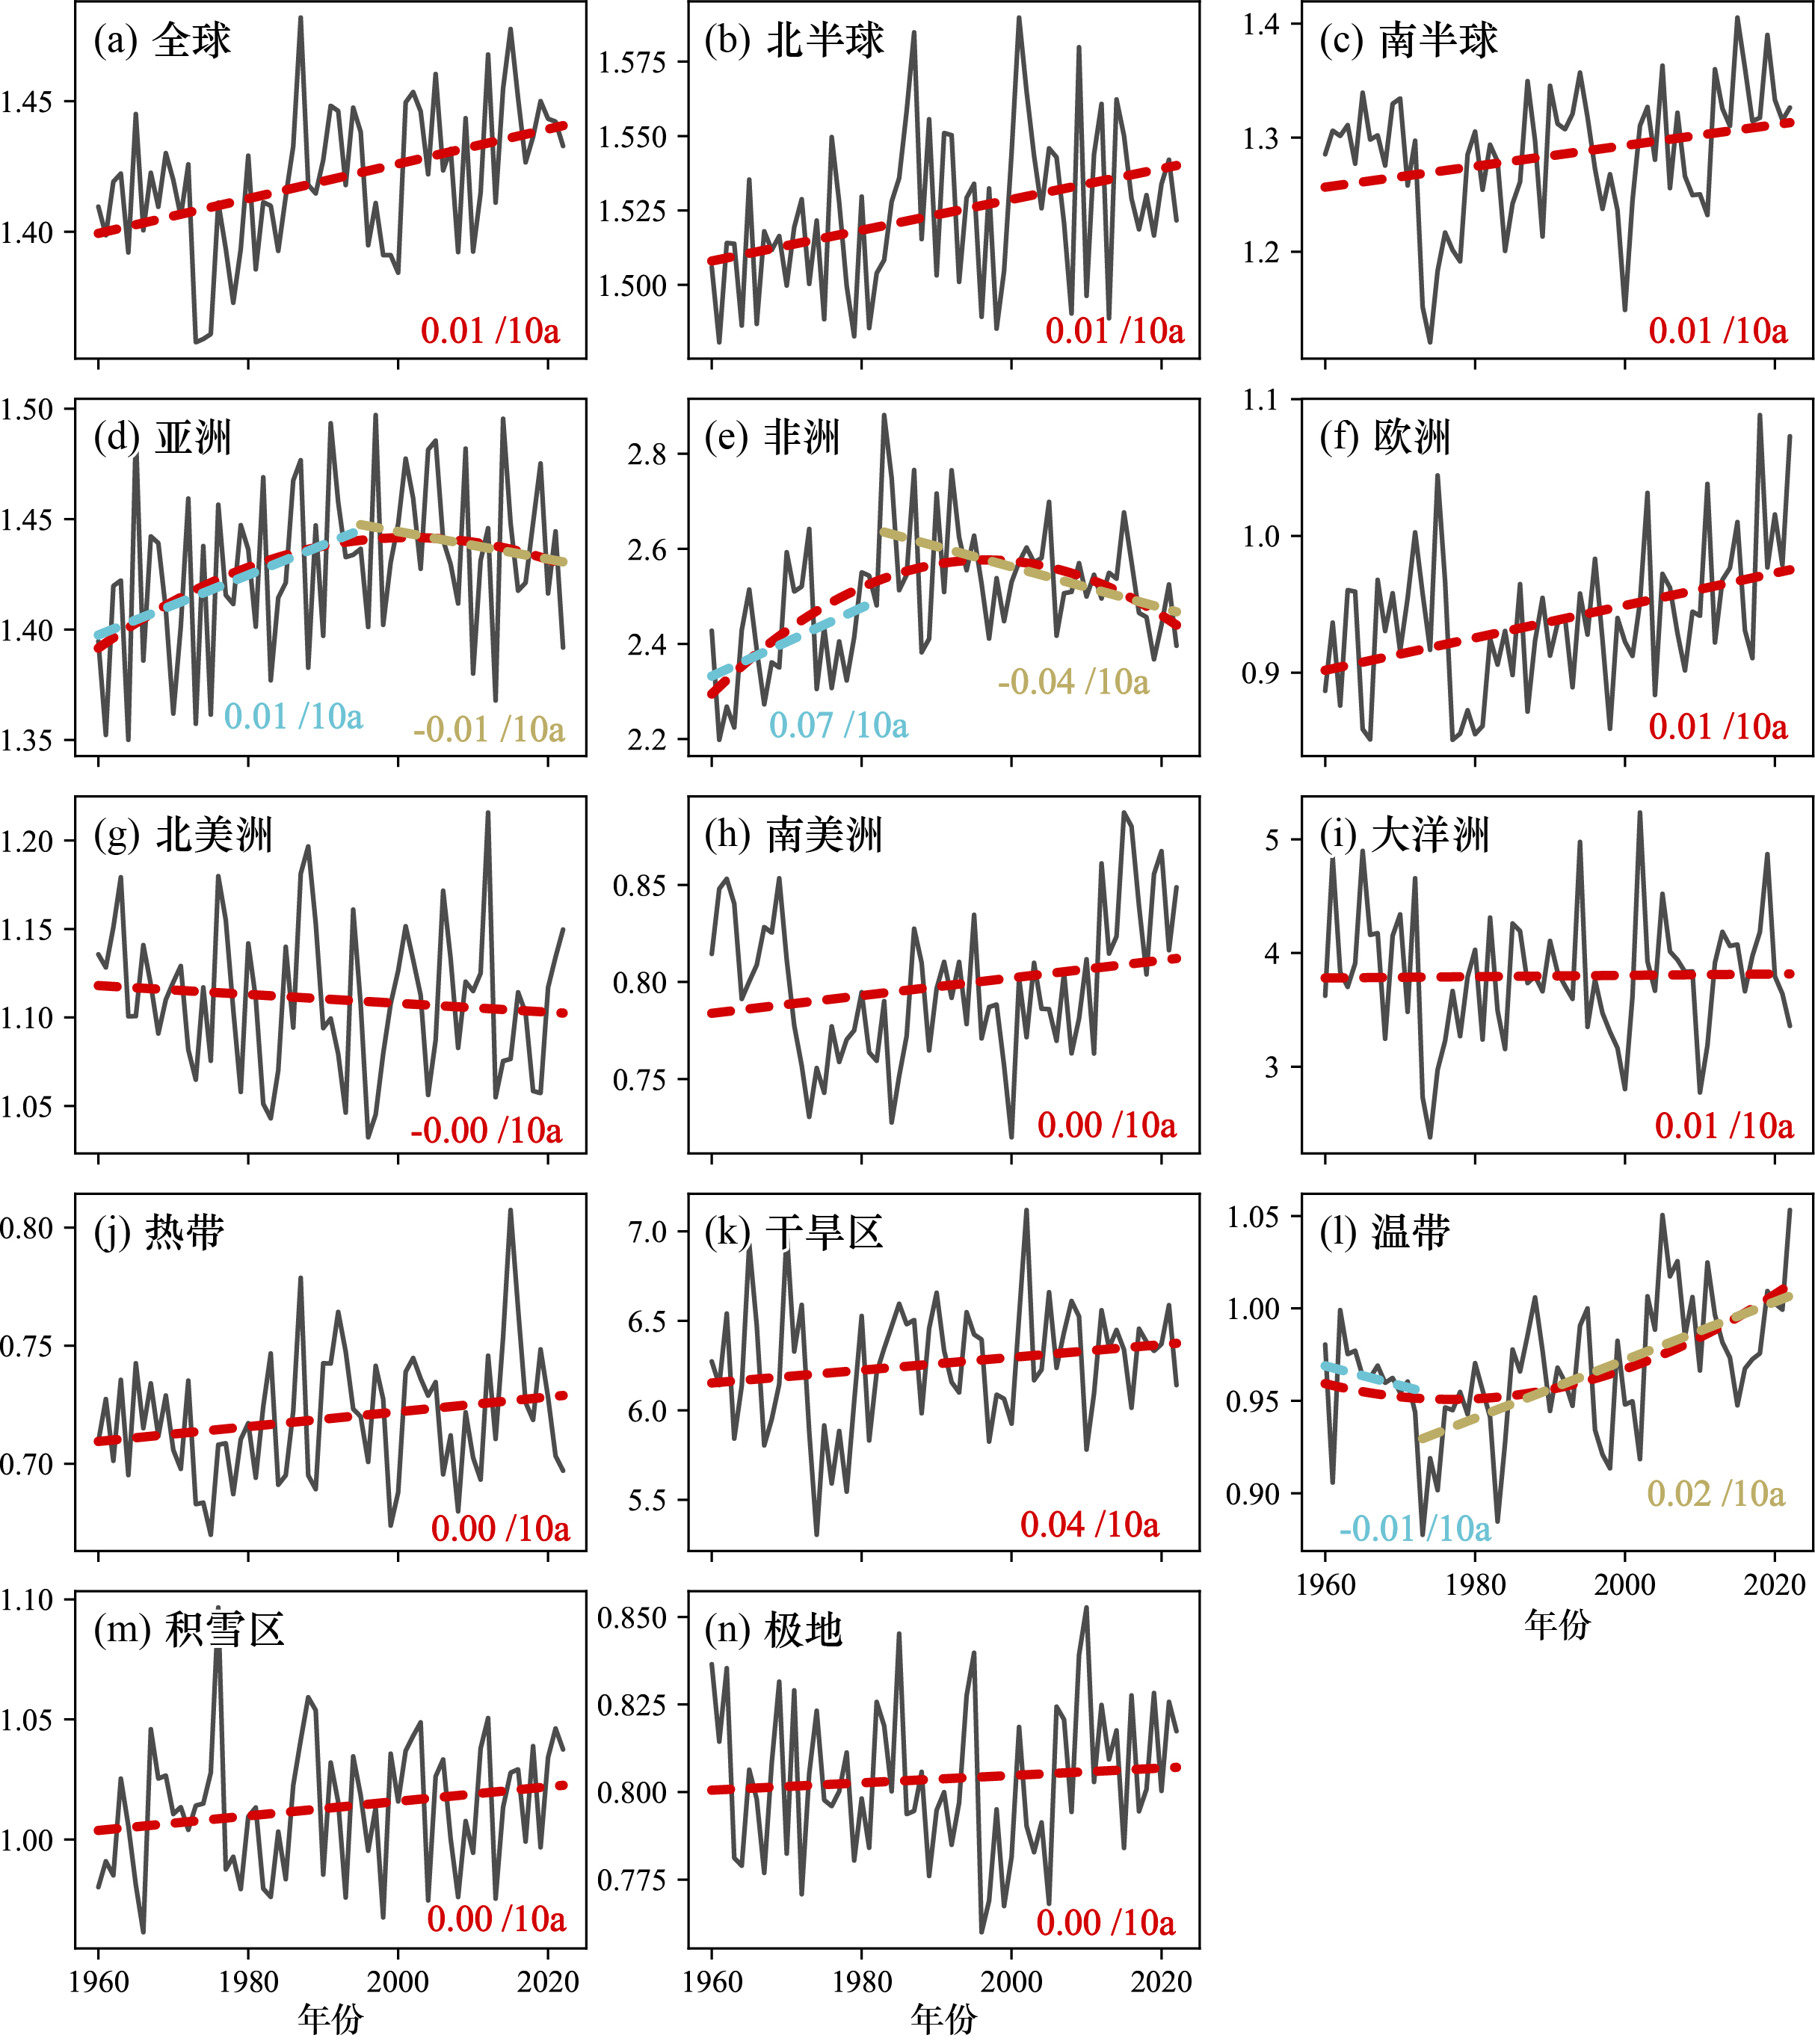
\includegraphics[width=0.85\textwidth]{figures/chap3/1_AI_Series.jpg}
% 	\bicaption{全球及区域干燥度指数序列及变化趋势}{Aridity index series and linear trend in global and regional scale}
% 	\label{fig:AI_Series}
% \end{figure}

% \begin{figure}[H]
% 	\centering
% 	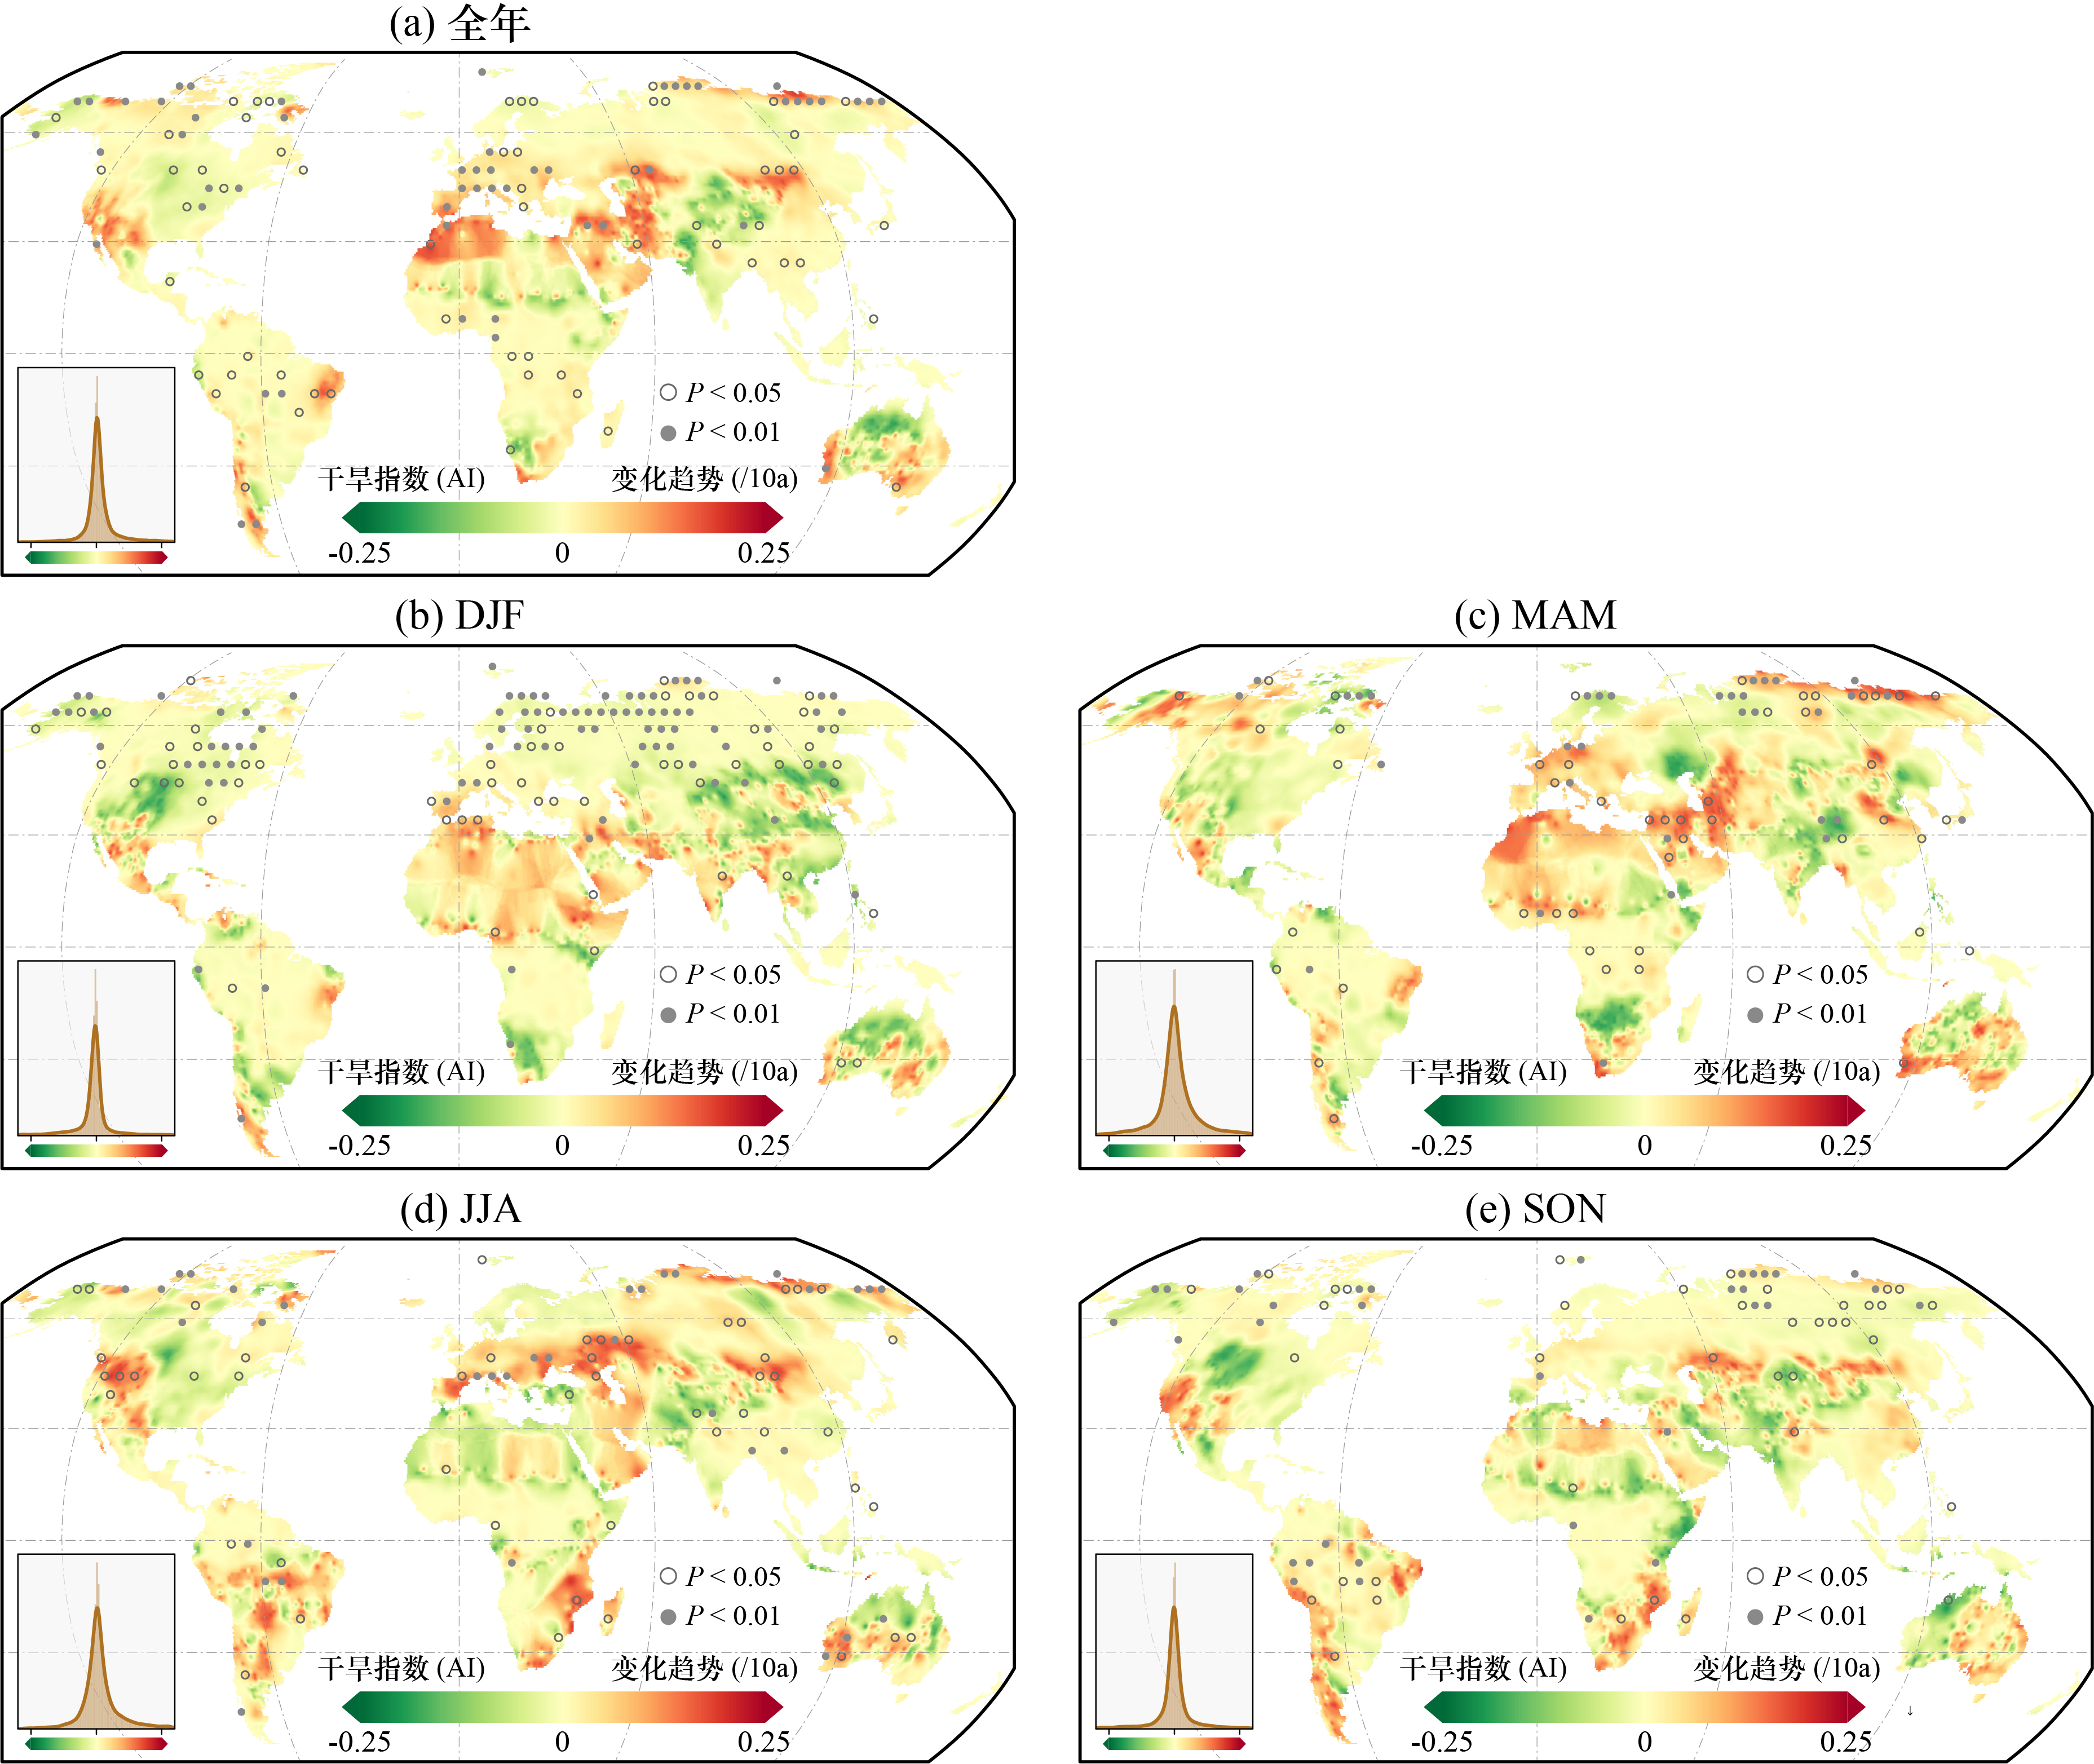
\includegraphics[width=0.85\textwidth]{figures/chap3/1_AT.jpg}
% 	\bicaption{全球年、季尺度干燥度指数变化空间格局}{Spatial pattern of annual and seasonal aridity index trend}
% 	\label{fig:AI_Trend_Map}
% \end{figure}

% \begin{figure}[H]
% 	\centering
% 	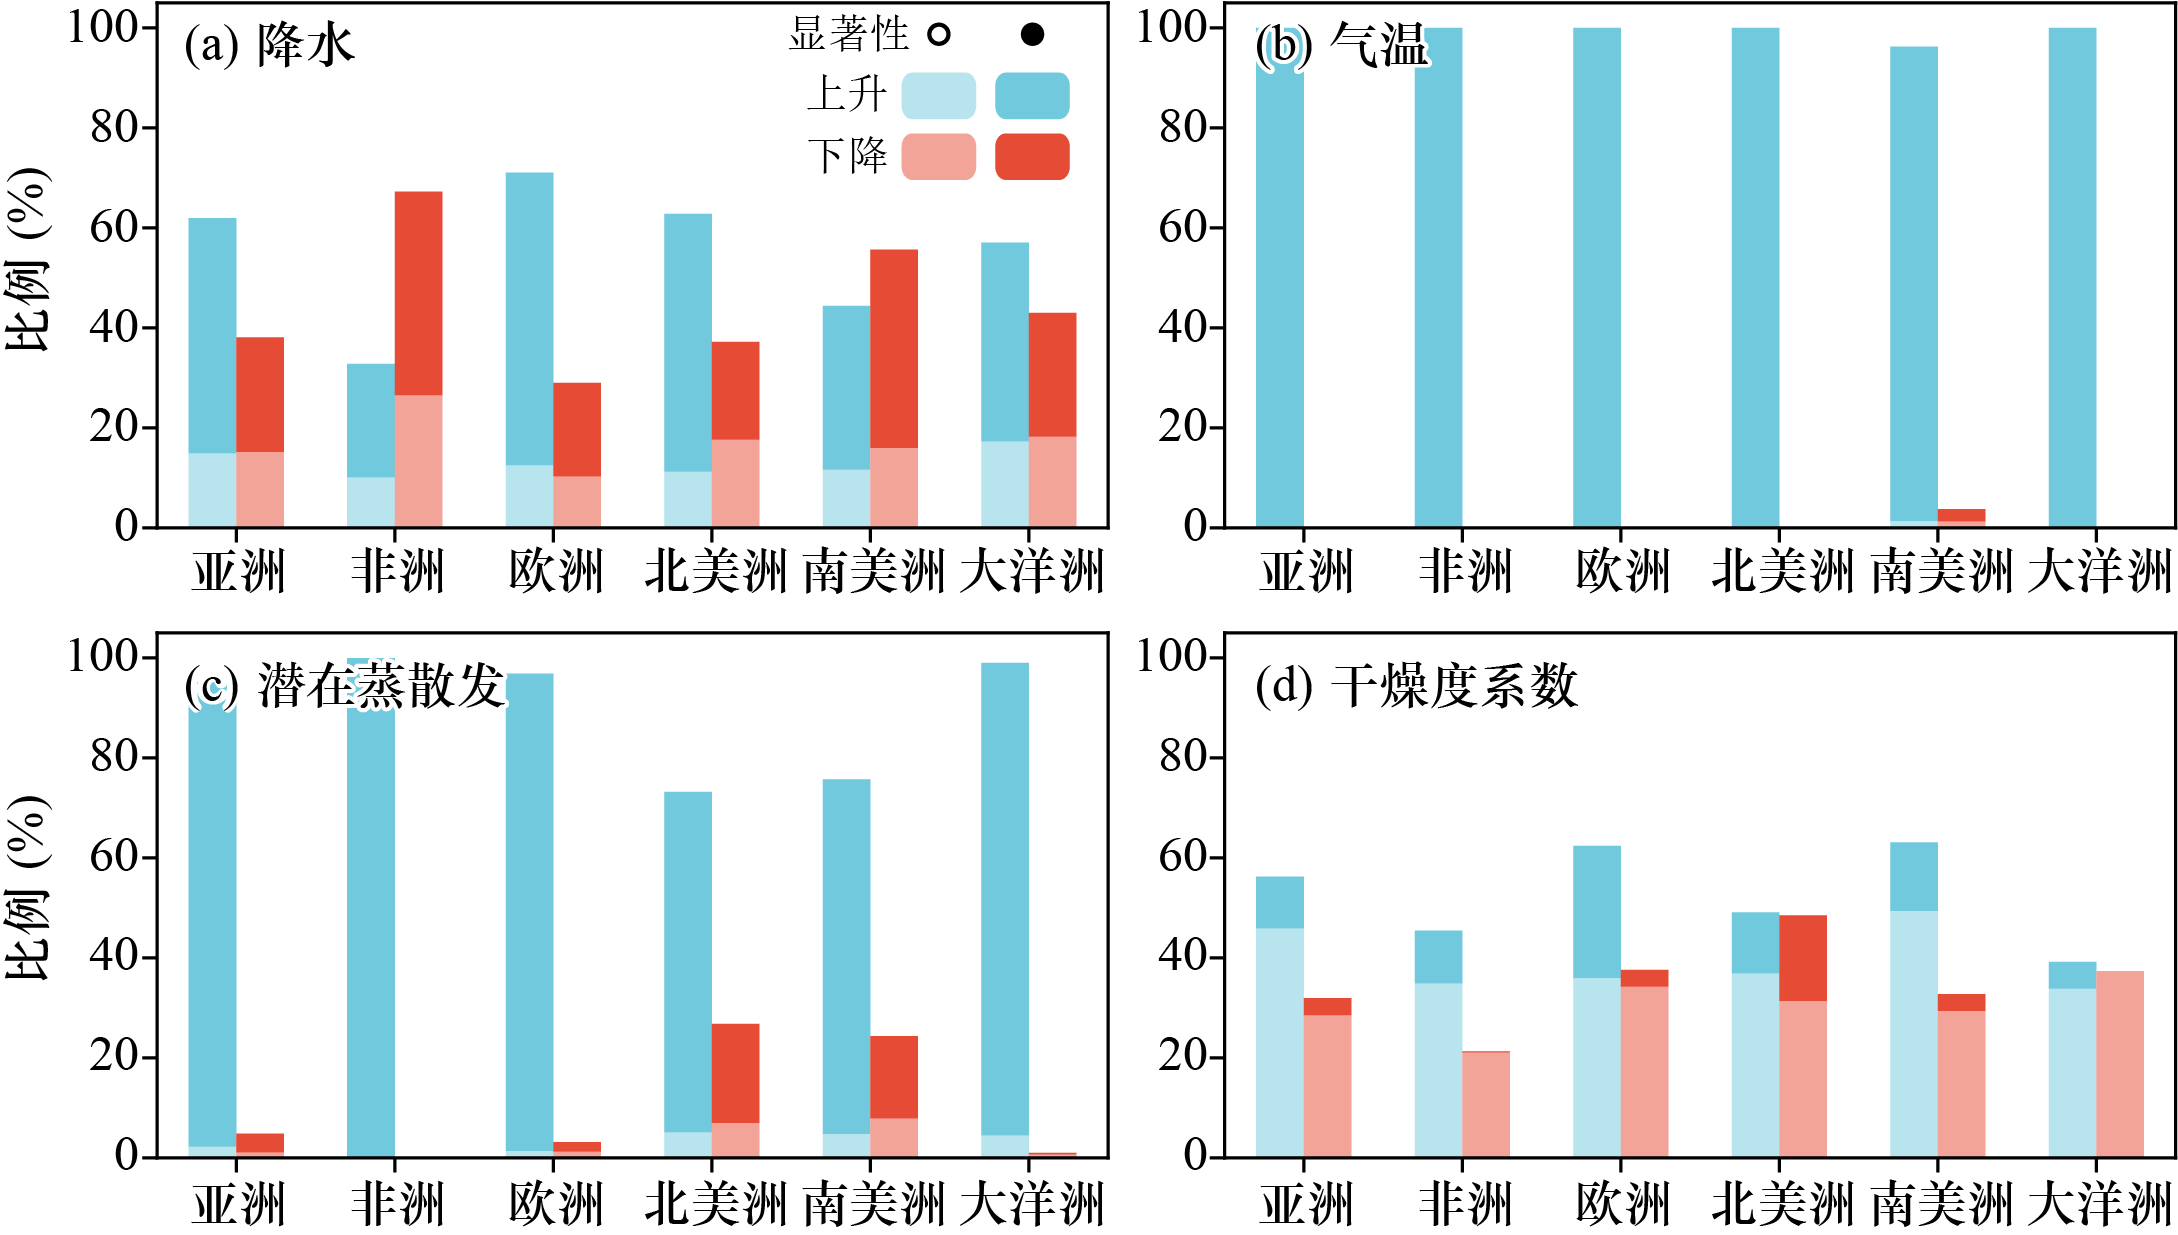
\includegraphics[width=0.85\textwidth]{figures/chap3/1_Trend_Stat_Conti.jpg}
% 	\bicaption{各大洲气候要素变化趋势统计}{Statistic of climatic contidions change for each continents}
% 	\label{fig:Trend_Stat_Conti}
% \end{figure}

% \begin{figure}[H]
% 	\centering
% 	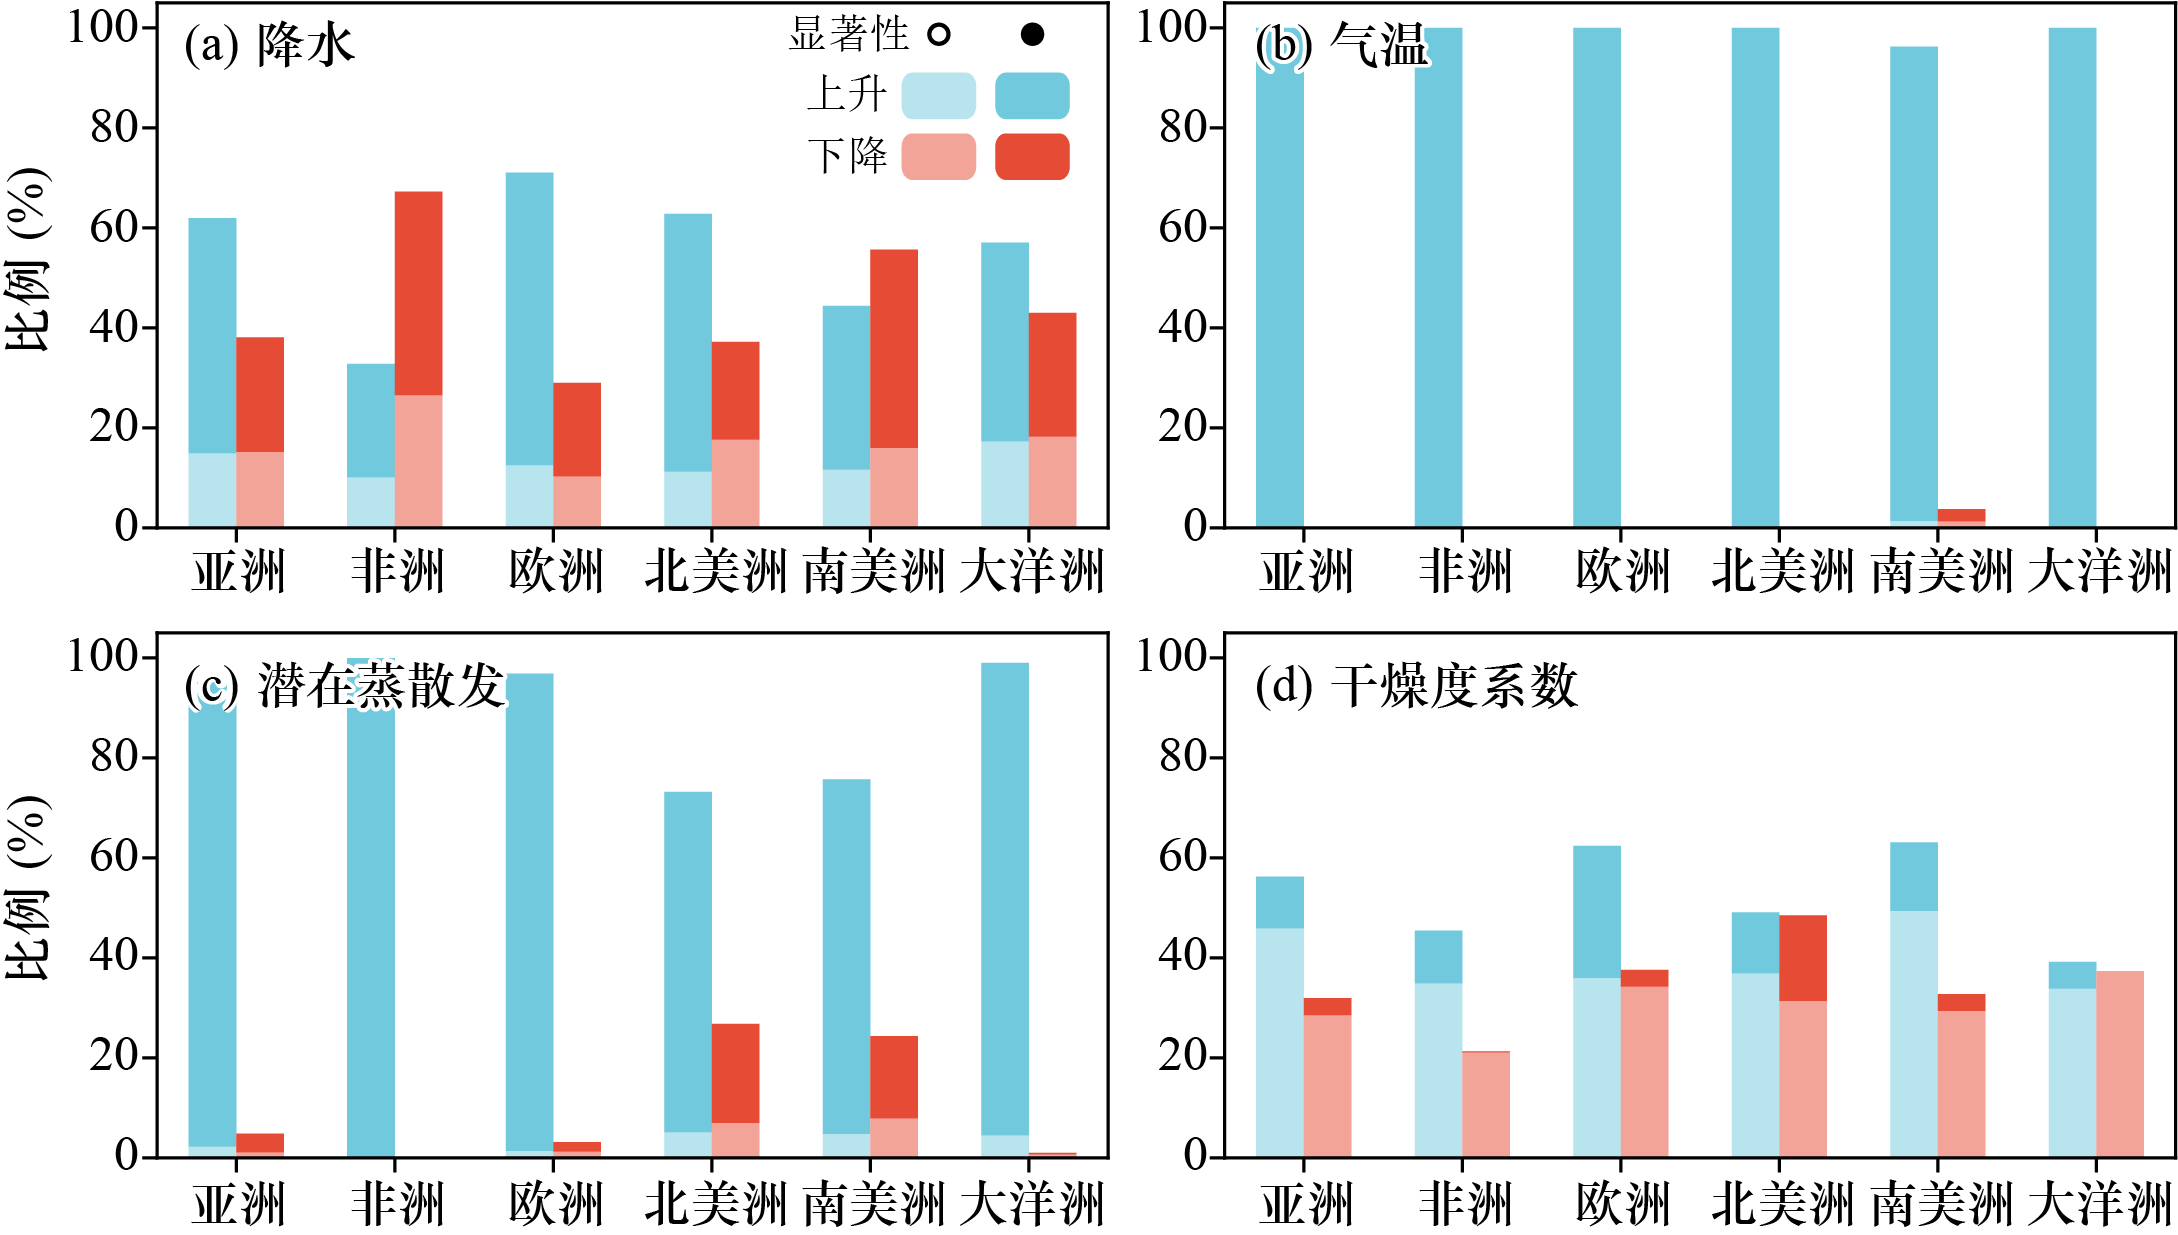
\includegraphics[width=0.85\textwidth]{figures/chap3/1_Trend_Stat_Conti.jpg}
% 	\bicaption{各气候区气候要素变化趋势统计}{Statistic of climatic contidions change for each climatic zones}
% 	\label{fig:Trend_Stat_Clim}
% \end{figure}

% \subsection{区域尺度气候要素的线性-非线性演变特征}

% \begin{figure}[H]
% 	\centering
% 	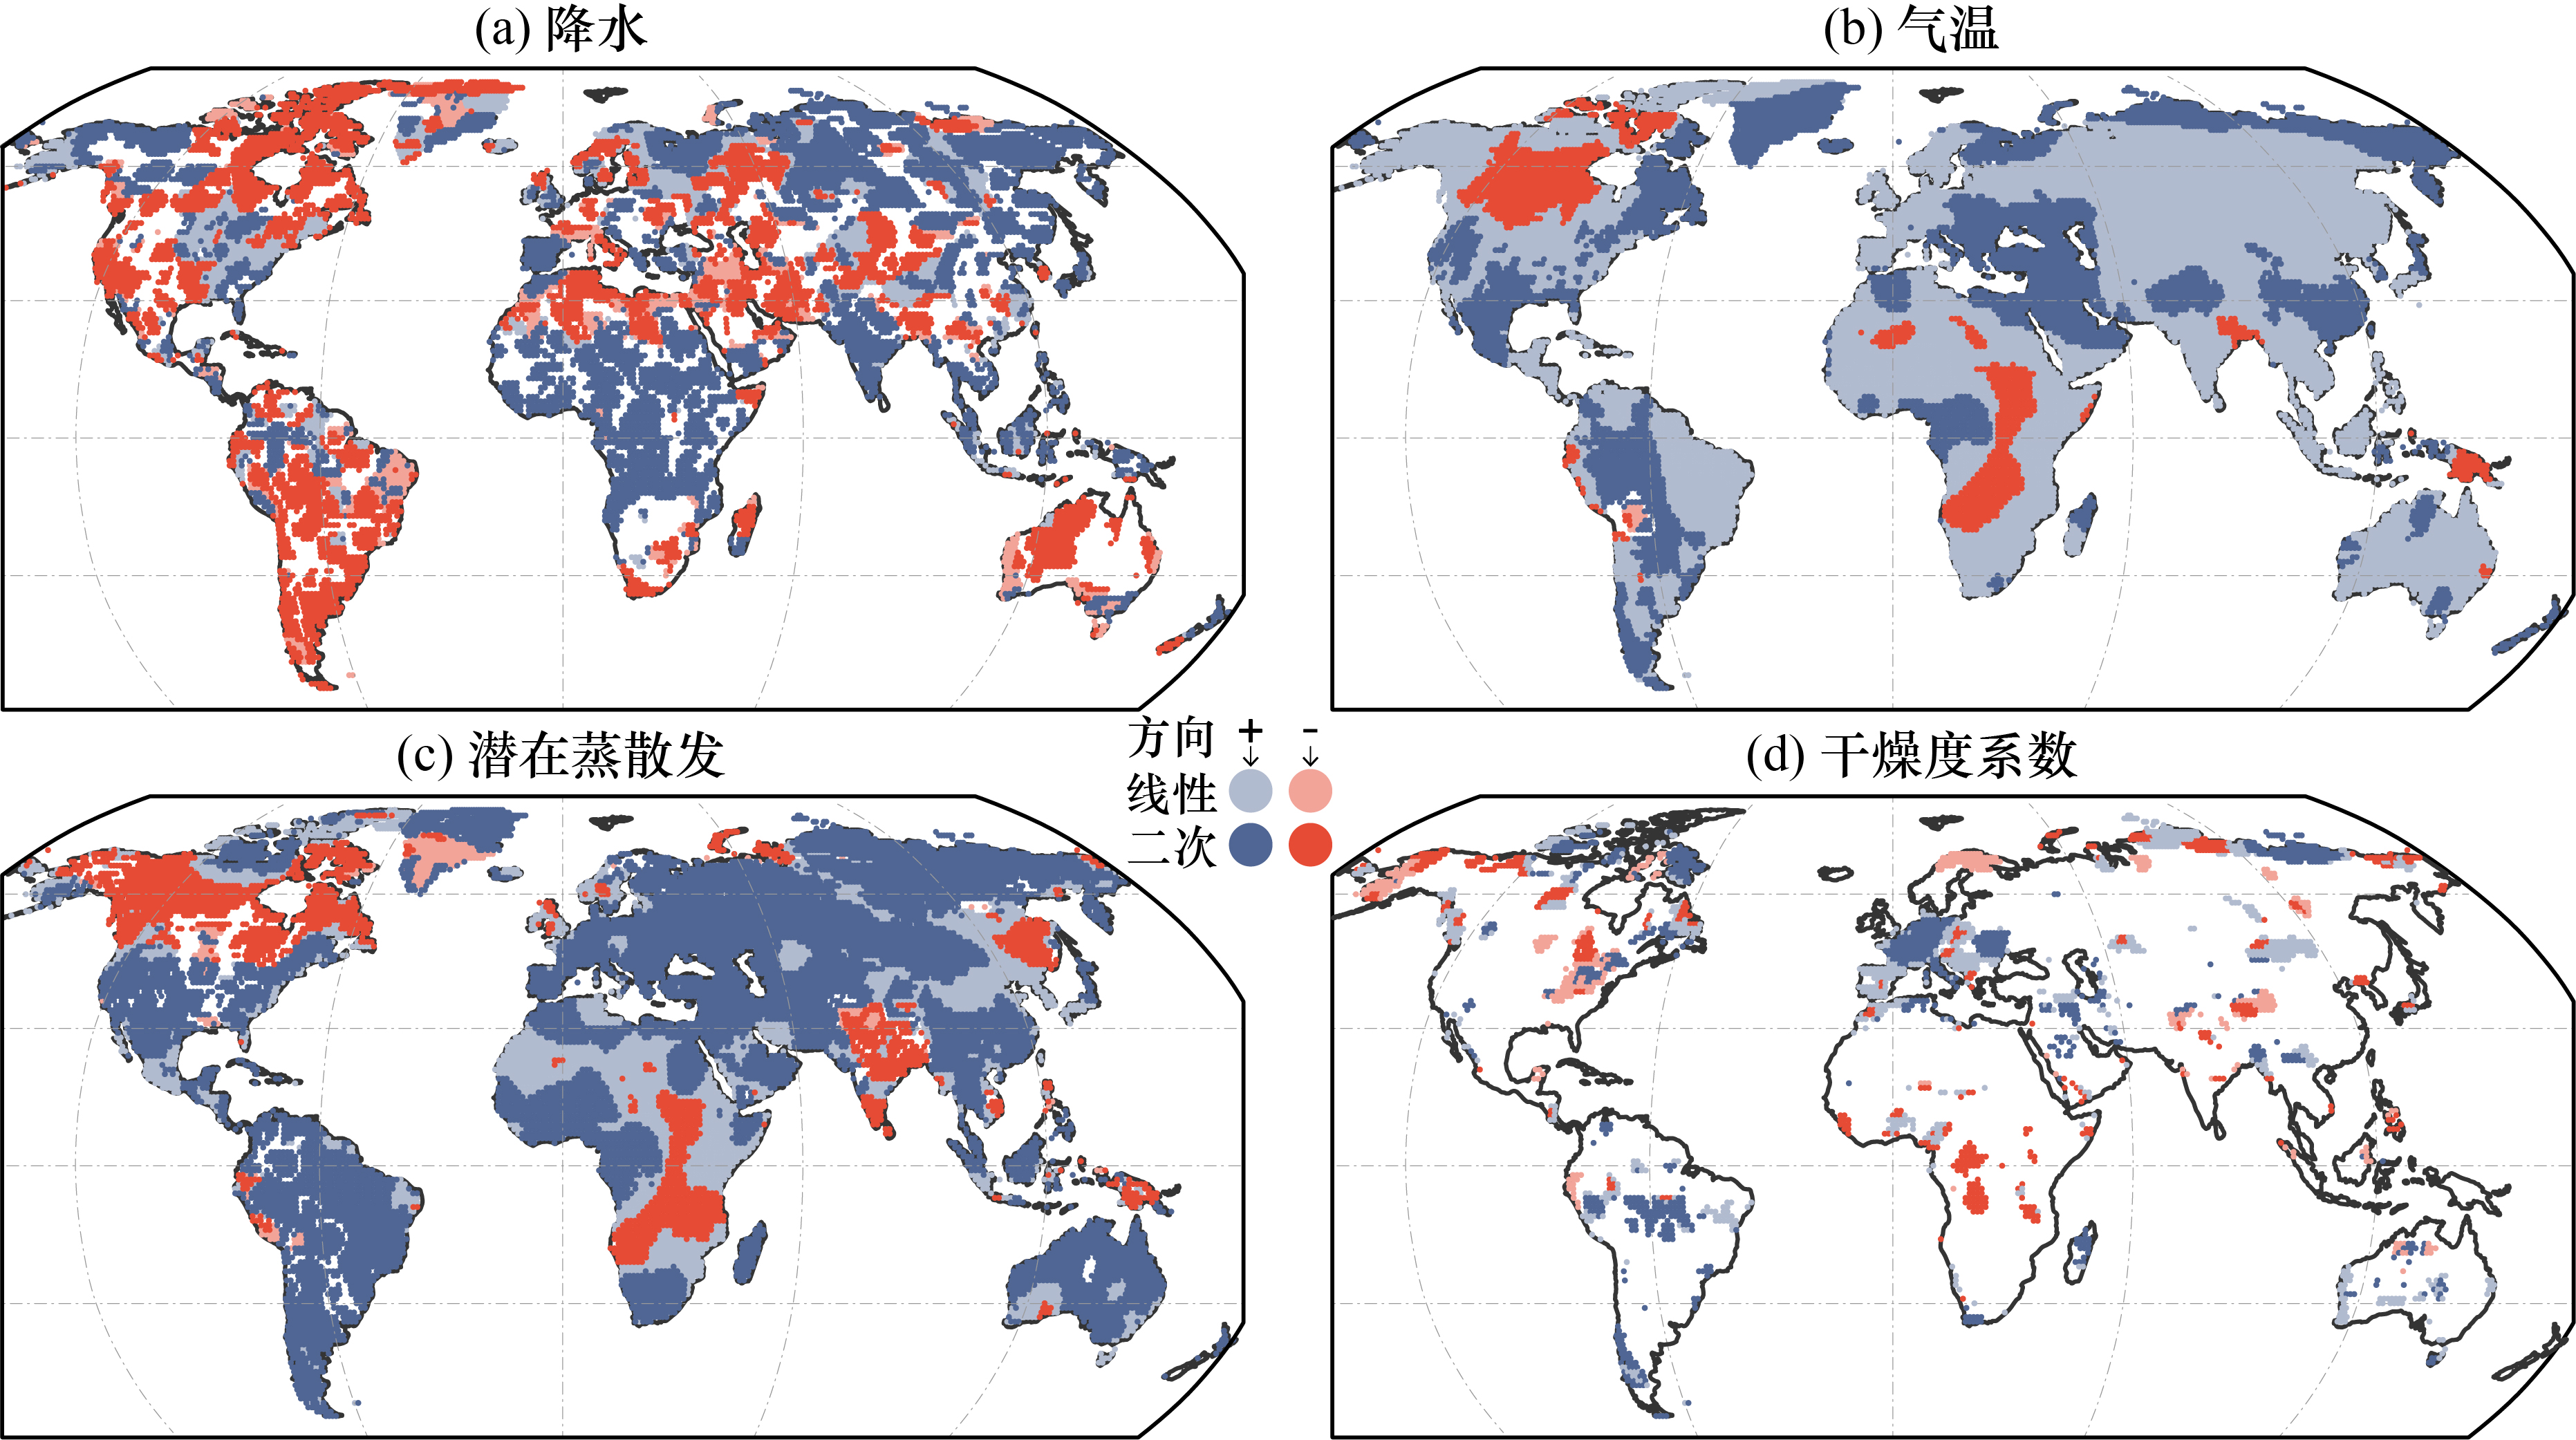
\includegraphics[width=0.85\textwidth]{figures/chap3/1_LNL_Map.jpg}
% 	\bicaption{全球气候要素线性-非线性变化空间格局}{Spatial pattern of climatic trend direction and linear-nonlinear trend type}
% 	\label{fig:LNL_Map}
% \end{figure}

% \begin{figure}[H]
% 	\centering
% 	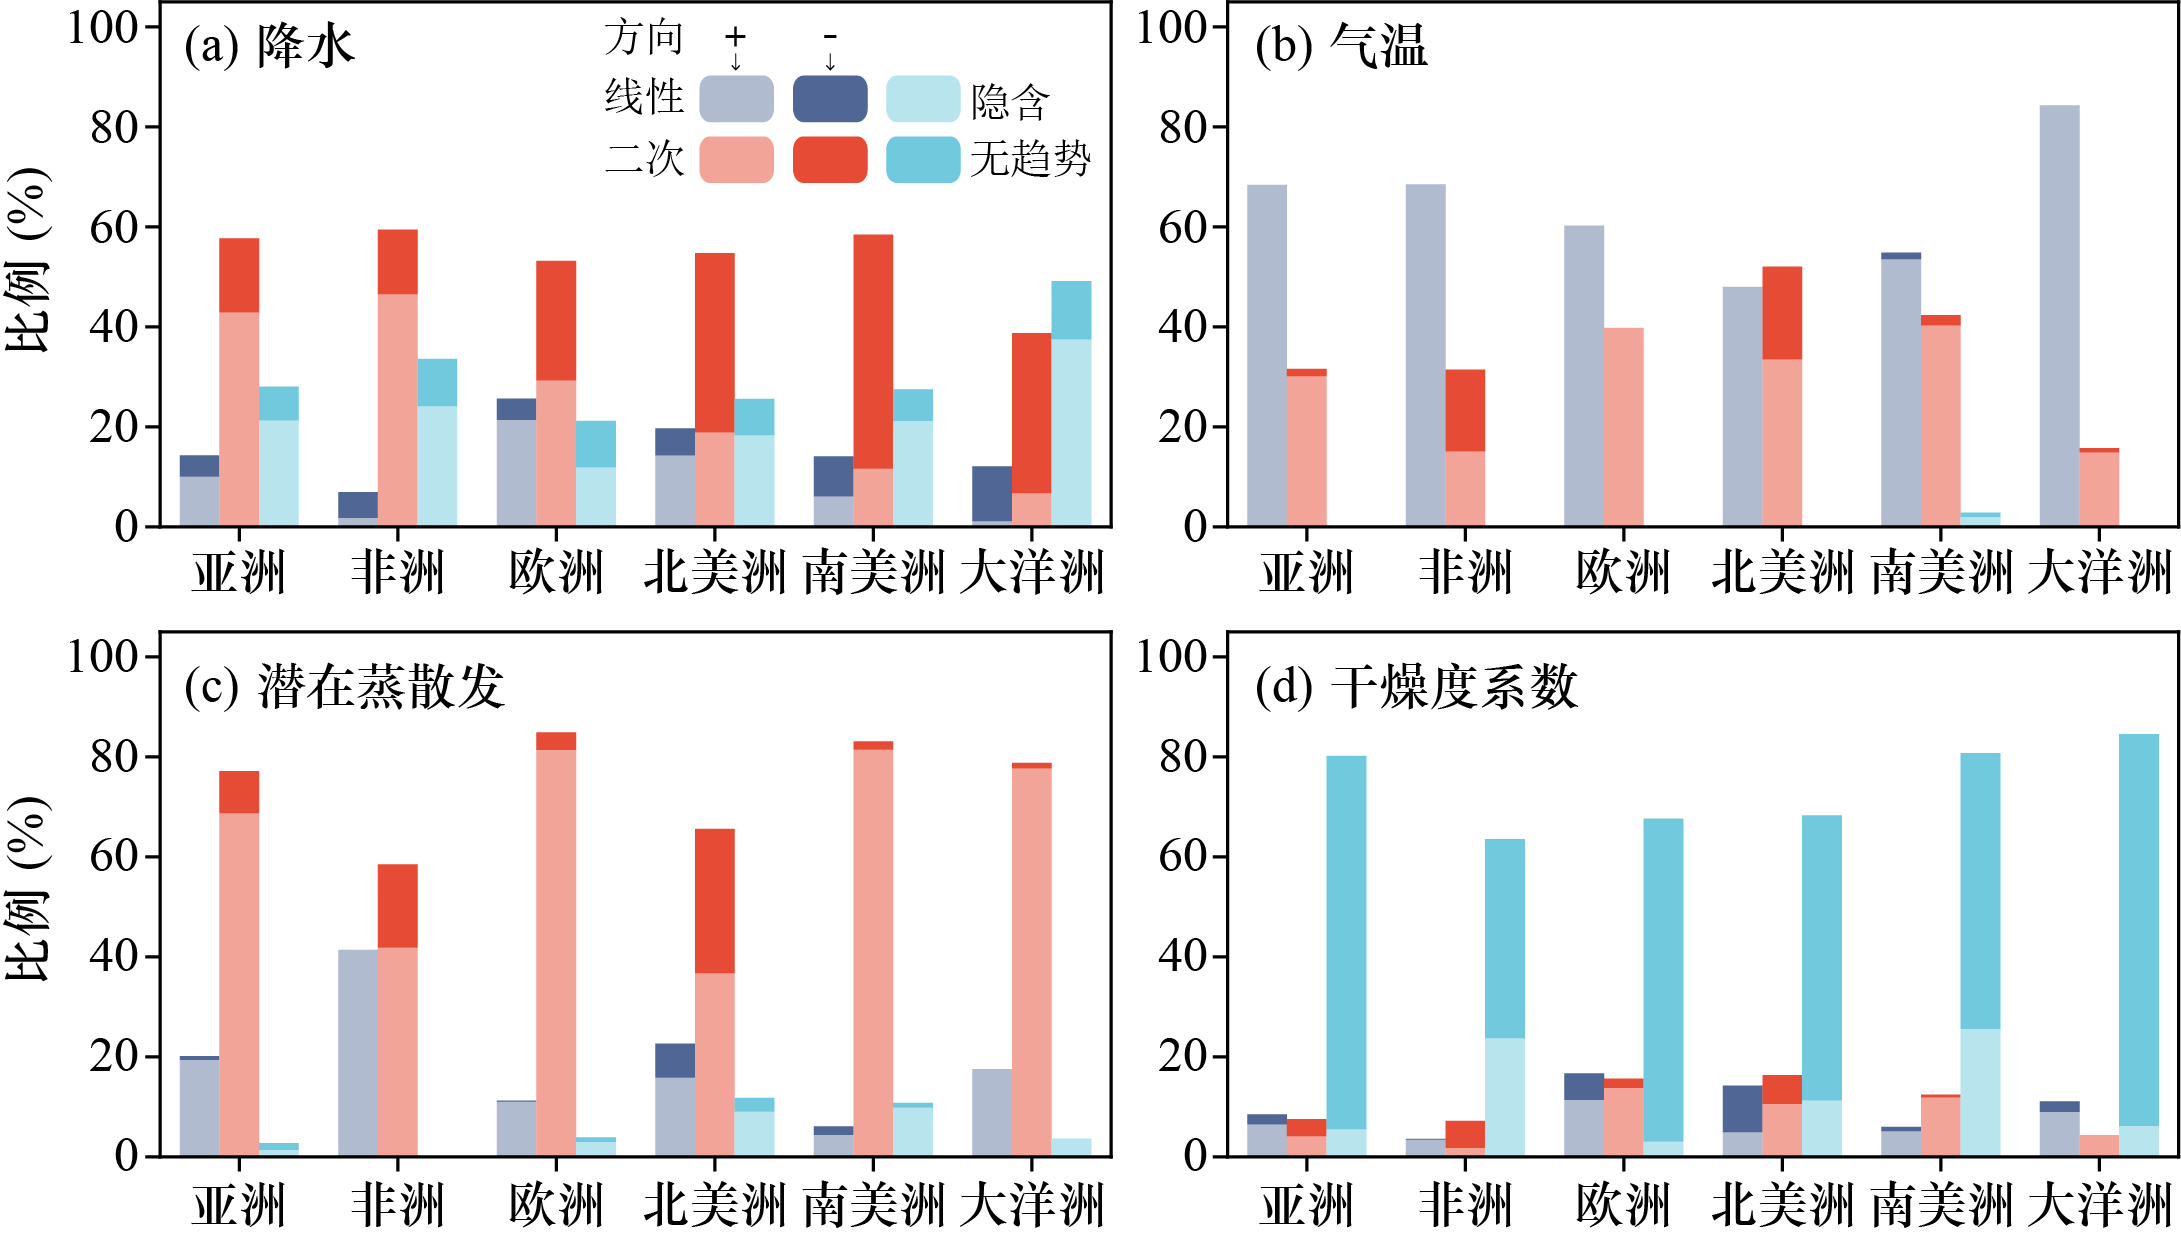
\includegraphics[width=0.85\textwidth]{figures/chap3/1_LNL_Stat_Conti.jpg}
% 	\bicaption{各大洲气候要素线性-非线性变化统计}{Statistic of trend direction and linear-nonlinear trend type for each continents}
% 	\label{fig:LNL_Stat_Conti}
% \end{figure}

% \begin{figure}[H]
% 	\centering
% 	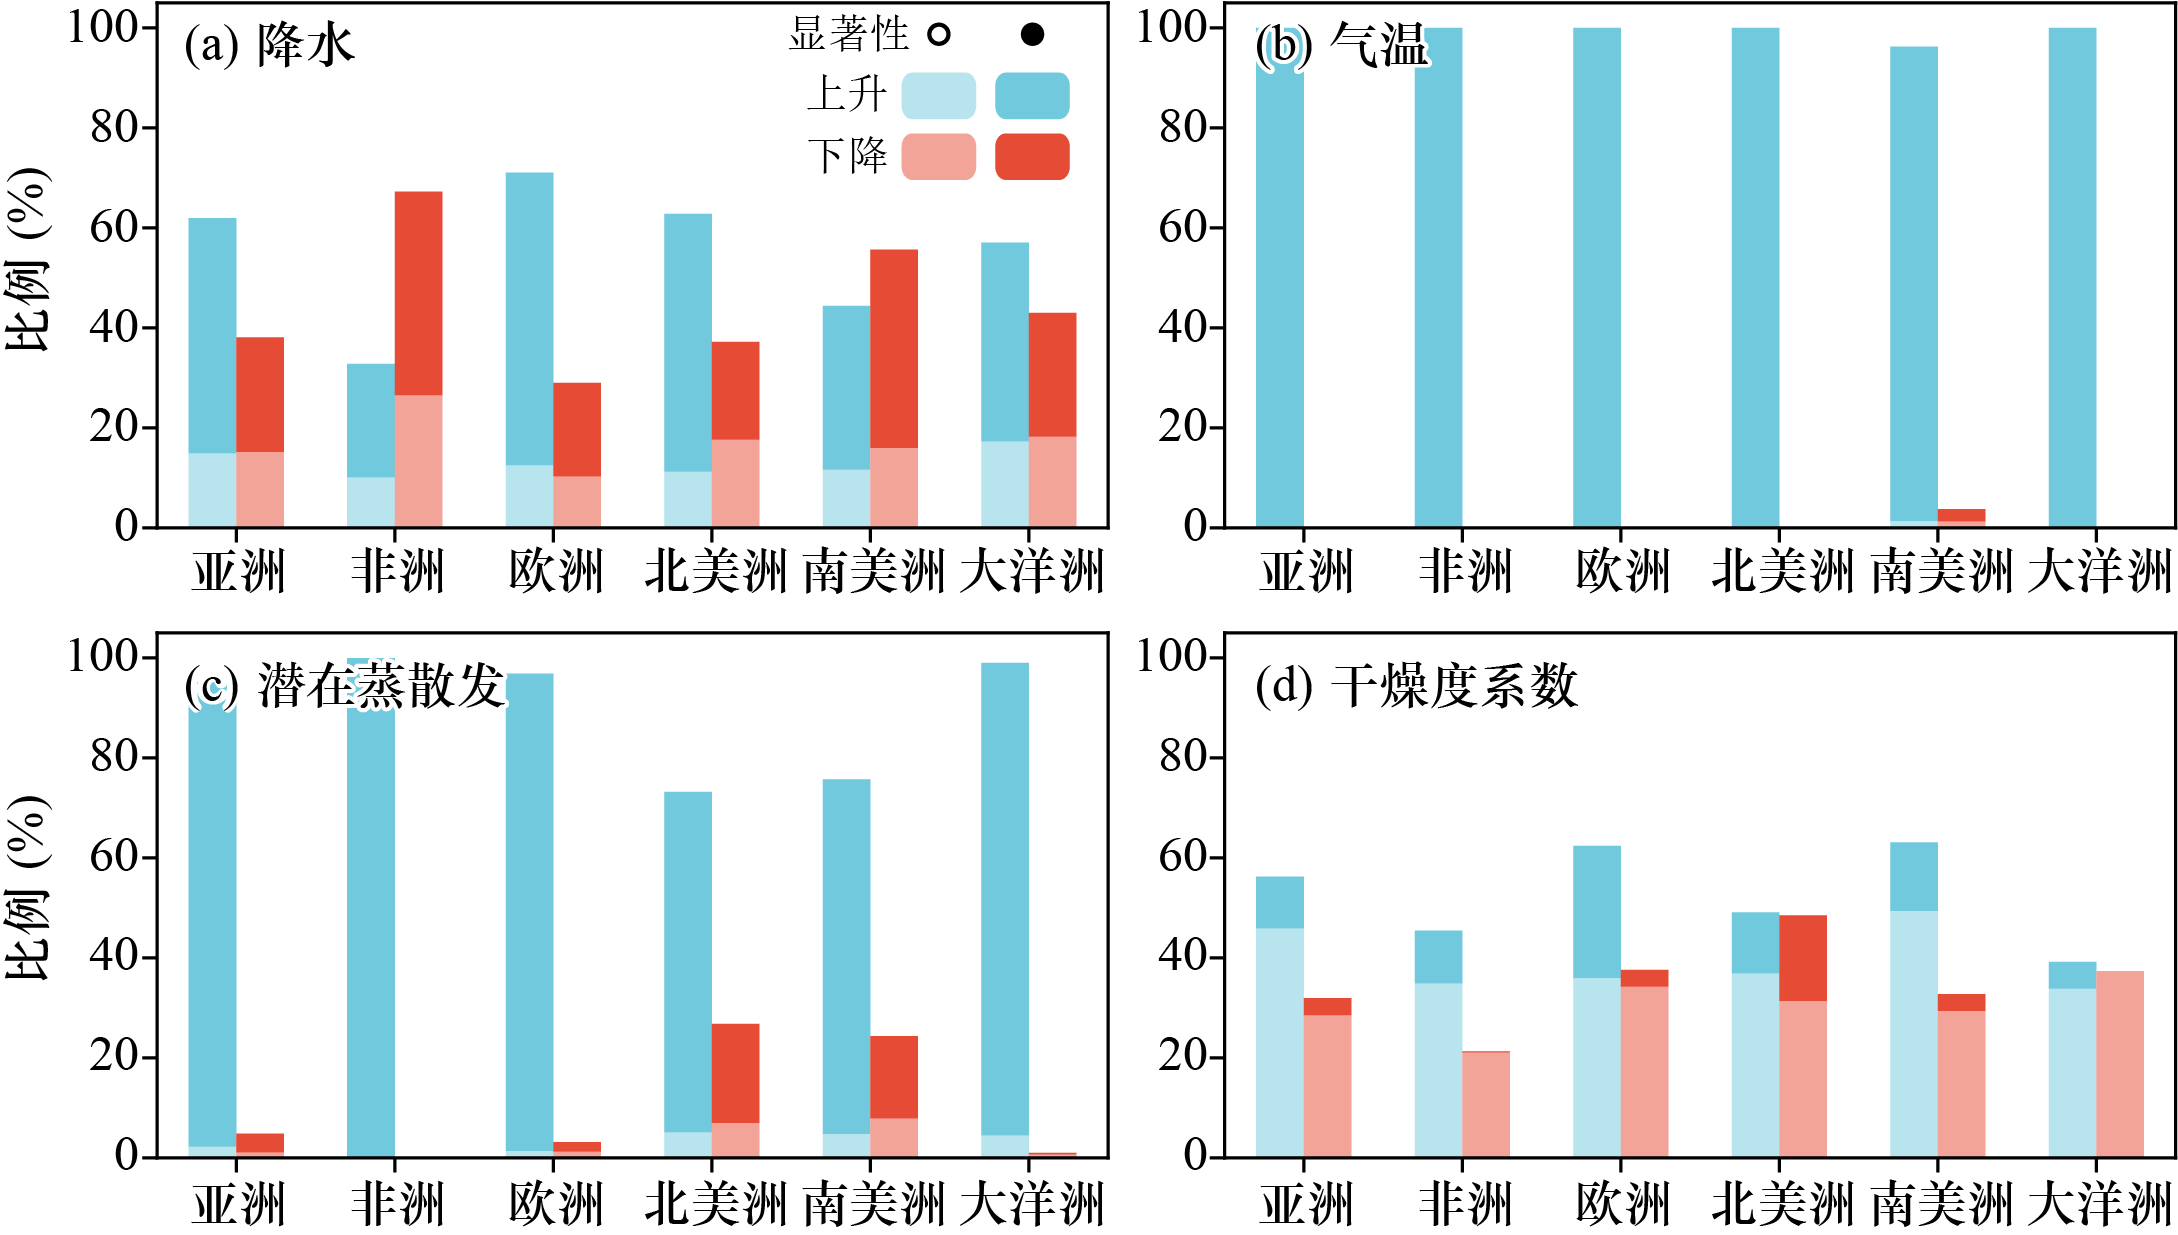
\includegraphics[width=0.85\textwidth]{figures/chap3/1_Trend_Stat_Conti.jpg}
% 	\bicaption{各气候区气候要素线性-非线性变化统计}{Statistic of trend direction and linear-nonlinear trend type for each climatic zones}
% 	\label{fig:LNL_Stat_Clim}
% \end{figure}

% \section{全球历史径流观测演变格局}

% \subsection{研究区域}

% 由于径流序列的分析需要一致的且具有一定长度的时间序列,并且对于缺失值敏感,研究的目的是评估不同区域在不同时间段内的径流演变规律。为了尽可能减少数据缺失和不确定性给分析带来的影响,同时尽量保证测试集水区的选择能够覆盖全球大多数陆地范围,以下5个标准被用于在所有数据集(全球流域数据集中,GRDC提供的10829站点,GSIM提供的30595站点和中国径流数据集中54个站点,共41842各占)中筛选可用于研究的流域。
% \begin{enumerate}
%     \item 删除GSIM与GRDC数据集中的重复站点。在此步骤中,10611个流域被排除在研究区之外。
%     \item 删除数据序列较短的站点,包括:
%     \begin{enumerate}
%         \item 径流序列少于15年。
%         \item 径流序列终止日期早于1900年。
%         \item 径流序列起始日期晚于2000年的站点。
%     \end{enumerate}
%     \qquad 在此步骤中,9983个流域被排除在研究之外。
%     \item 删除数据序列中缺失值较多的站点,包括:
%     \begin{enumerate}
%         \item 数据中NaN(无效值)占比超过50\%。
%         \item 数据中0占比超过50\%。
%         \item 数据中0和NaN总占比超过50\%。
%         \item 连续180个数据中0和NaN占比超过70\%
%         \item 最大值和最小值之差小于2。
%     \end{enumerate}
%     \qquad 在此步骤中,8926个流域被排除在研究之外。
%     \item 删除流域面积小于5km\textsuperscript2的流域以排除过小流域和GSIM中流域边界计算错误。在此步骤中,共有6926个流域被排除在研究之外。
%     \item 删除集水区边界中不包含CRU气候数据格点的站点,以此保证流域气候条件的数据可用性。在此步骤中,955个流域被排除在研究之外。
% \end{enumerate}\par
% 经过上述准测筛选后,共有13627个流域被包含在本章节的研究范围内,如图\ref{fig:Study_Area_Trend}所示。根据Gudmundsson等\cite{gudmundssonObservedTrendsGlobal2019}提出的准则,包含了超过50个研究流域的次大陆区域再研究中被认为是充分的。图中统计了各个区域包含的流域数量,包含了超过50个流域的次大陆区域在图中以红色边框标出,共有31个区域被选出。

% \begin{figure}[H]
% 	\centering
% 	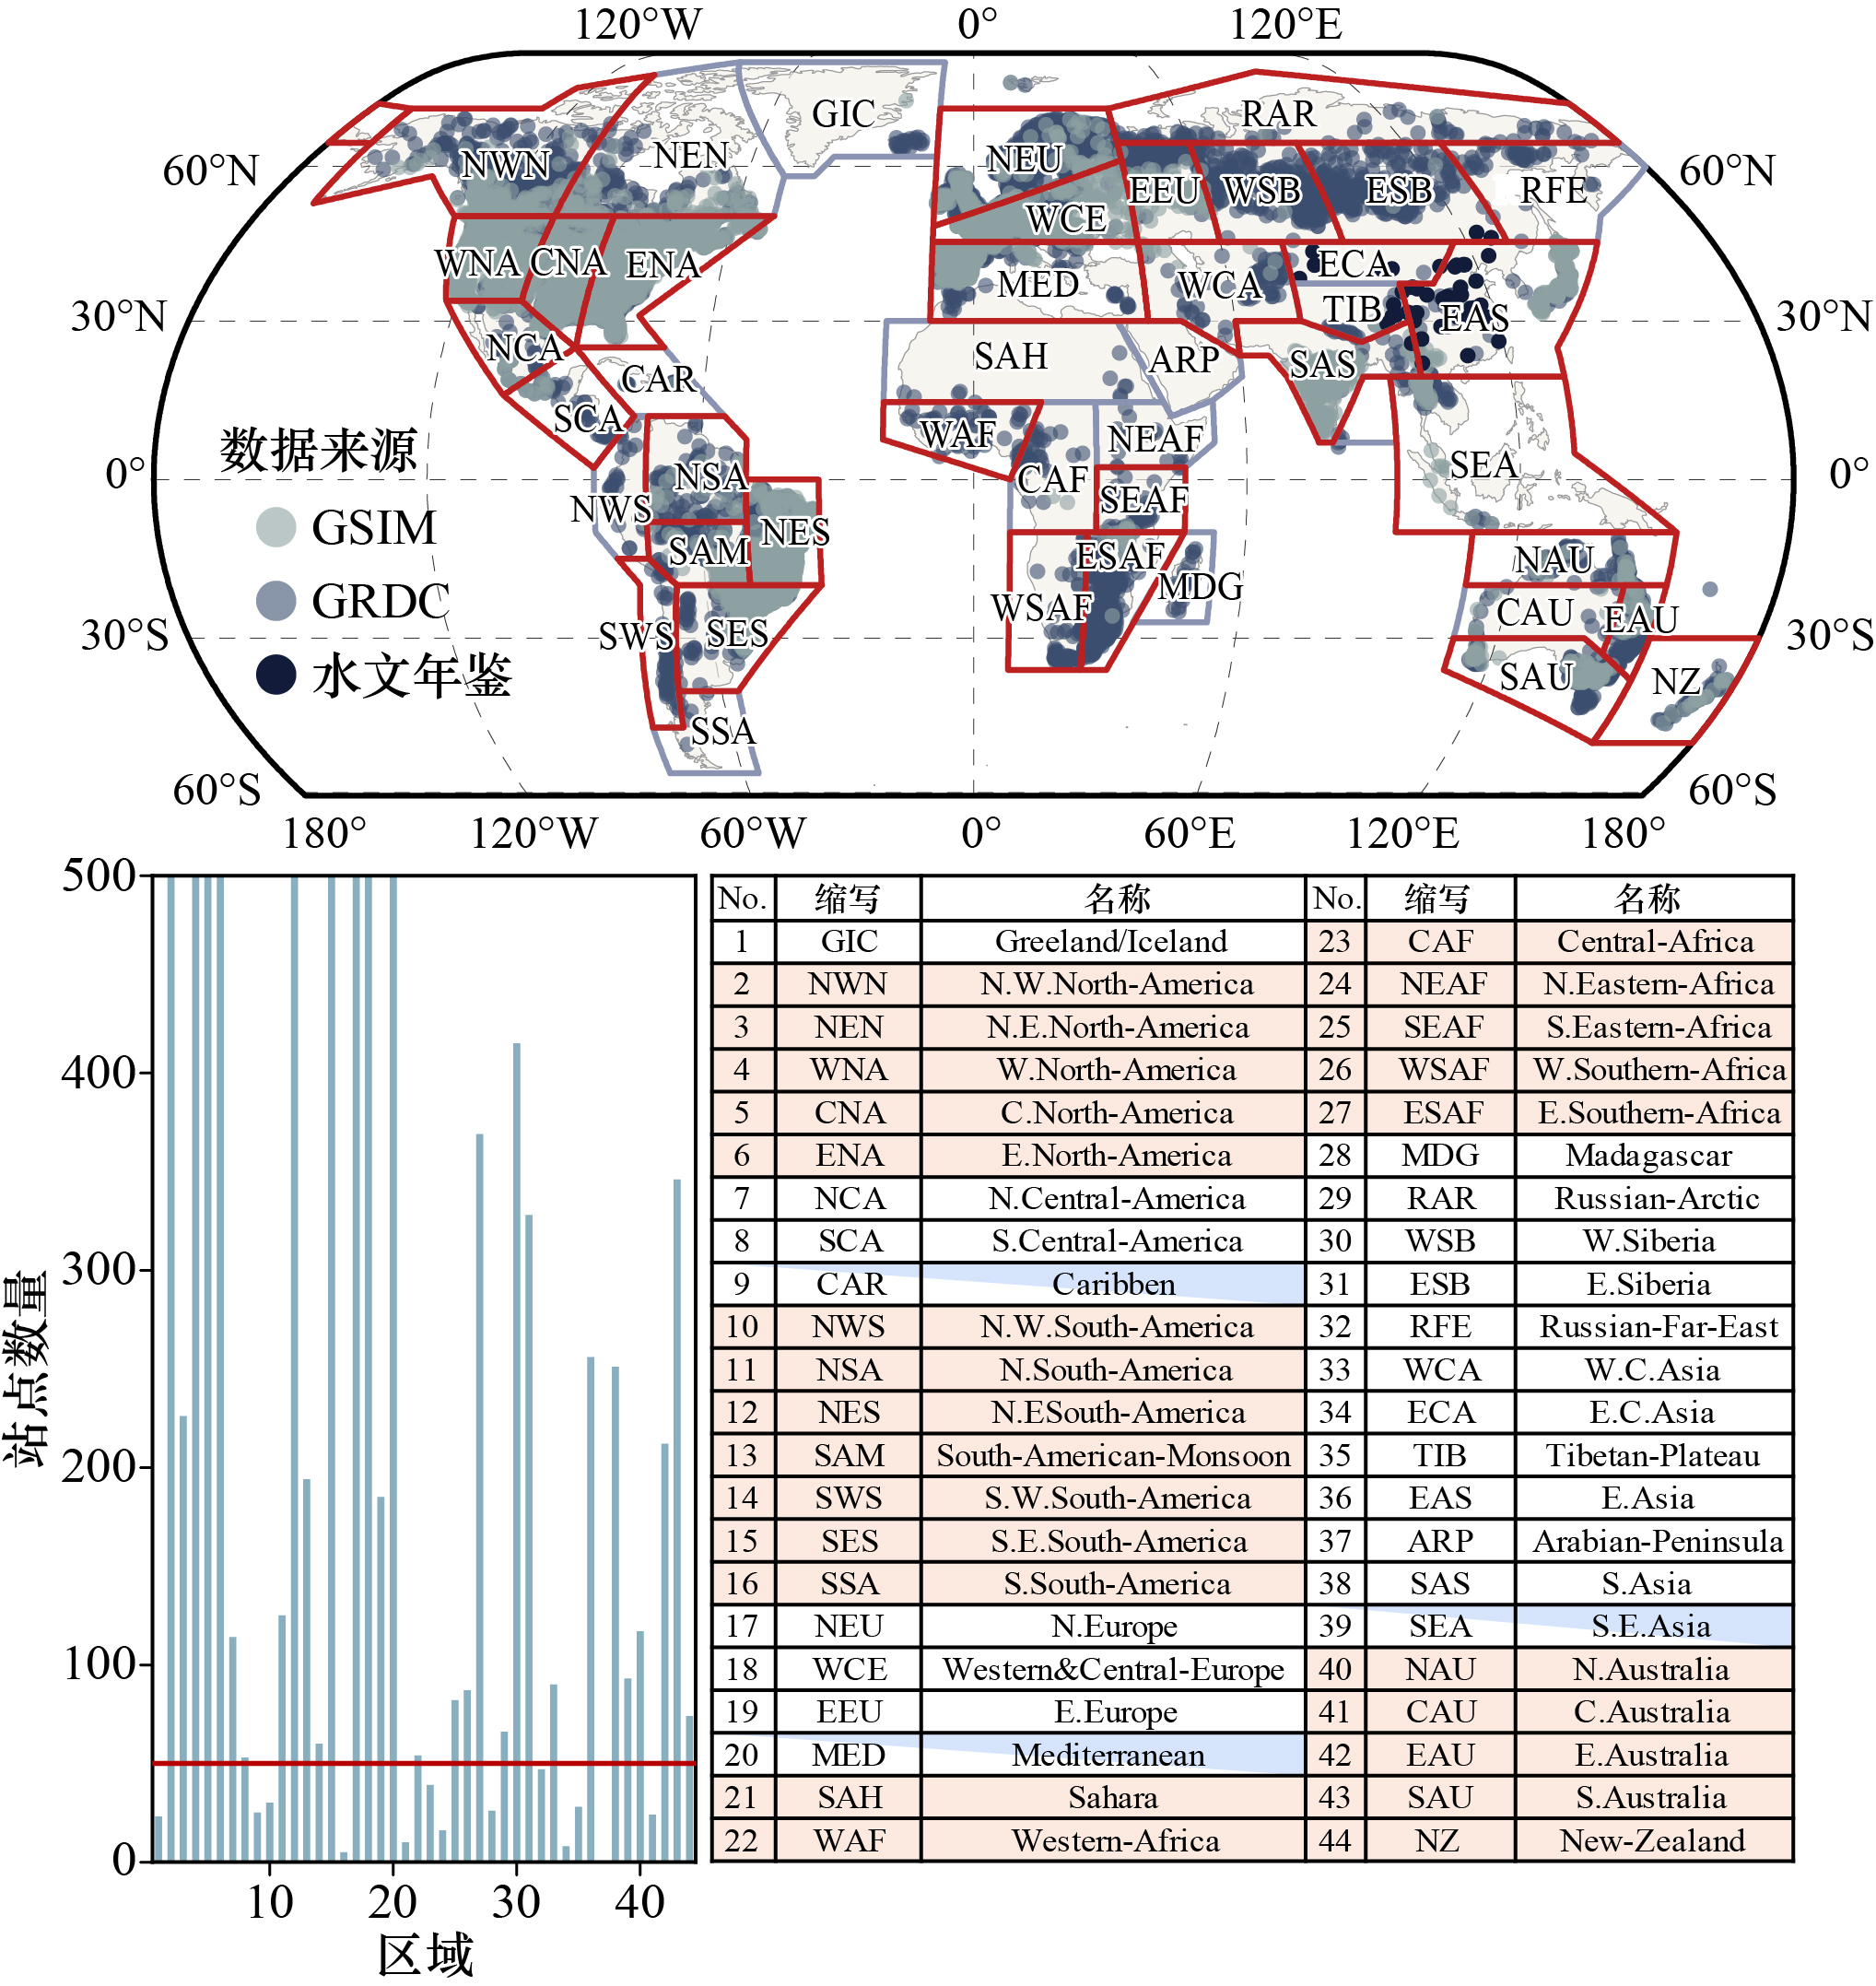
\includegraphics[width=0.85\textwidth]{figures/chap3/0_Study_Area_Trend.jpg}
% 	\bicaption{研究流域分布图}{Map of catchments involved in this chapter}\label{fig:Study_Area_Trend}
% \end{figure}

% \subsection{实测径流数据缺失值插补}

% 本节对全球范围内10799个流域的径流数据进行了缺失值和无效值的插补,平均缺失率为7.1\%,目的是保证BFAST算法的准确执行。对于每个流域,分别训练了三种机器学习模型,模型在训练集和测试集上的评估指标如图\ref{fig:Interp_Indices_Boxplot}所示。从NSE来看,三种模型在训练集上的表现都比较好,均在超过一半的流域得分超过0.5,其中XGB的表现最为优越,在超过75\%的流域中NSE超过了0.7。测试集上的表现相对于测试集较差,NSE普遍低于训练集,表明模型在测试集上的泛化能力有所降低,其中,XGB的性能下降最为明显,其次是RF,SVR的性能下降不显著,说明XGB的过拟合现象较为明显。从RE来看,RF和XGB在训练集都能比较精确的模拟出径流的水量特征,而SVR则存在明显的低估,在超过一半的流域径流模拟偏差超过了10\%。RMSE和CC指标表现出的规律与NSE和RE类似。三种模型在测试集上的表现比较相似,XGB在训练集上的性能最好,RF具有最高的稳定性,几乎不存在过拟合现象。\par

% \begin{figure}[H]
% 	\centering
% 	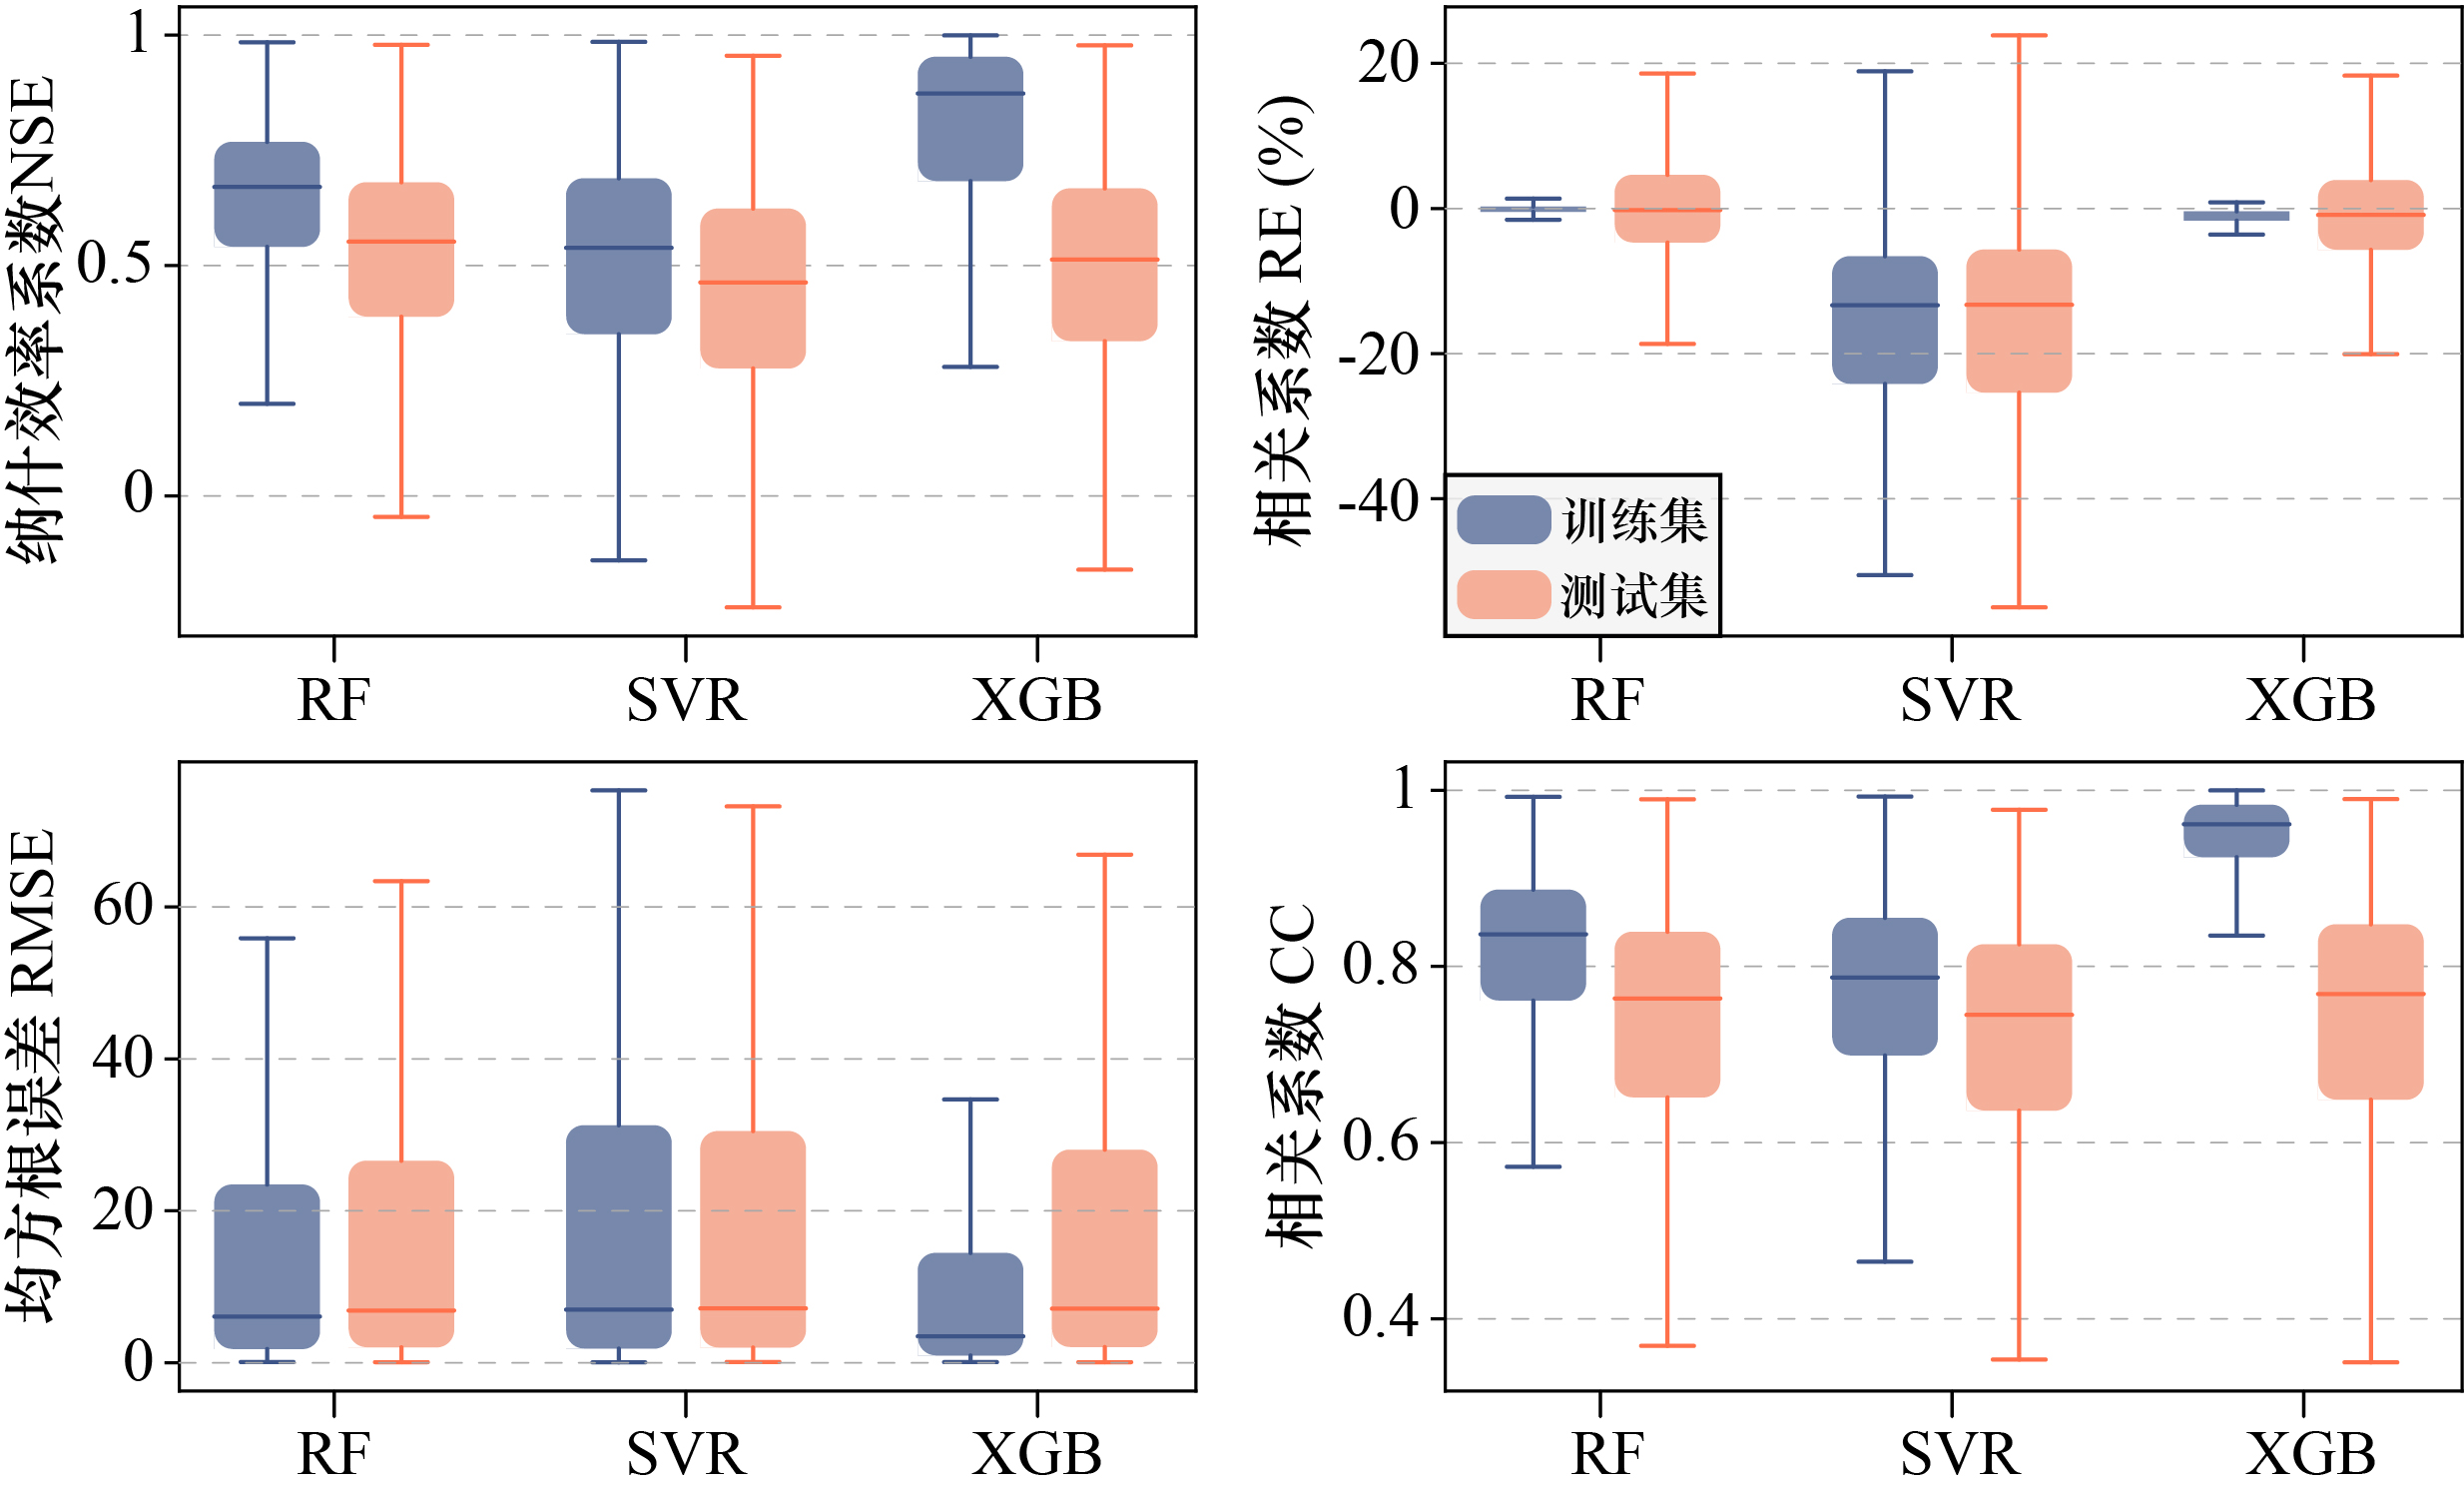
\includegraphics[width=0.85\textwidth]{figures/chap3/2_Interp_Indices_Boxplot.jpg}
% 	\bicaption{三种机器学习模型在训练集和测试集下的四种评估指标统计结果}{Four performance indices for three ML models in train set and test set}
%   \label{fig:Interp_Indices_Boxplot}
% \end{figure}

% 如图\ref{fig:Interp_TrTe_NSE_RE}所示,空间上看,RF和XGB在各个区域流域的测试集上表现都很好,大多数流域的NSE值都在0.6以上,尤其是在欧洲、北美和中国部分地区,但是在测试集的表现上,模型性能存在明显的空间异质性。在北美洲中部、欧洲东南部、大洋洲东南部等较为干旱的区域,模型的模拟结果较为失败,可能是由于这些地区复杂的水循环过程难以用简单的非线性机器学习模型进行概括\cite{ghiggiGRUNObservationbasedGlobal2019}三种模型在训练集上的RE值较低,大多数流域的RE值集中在-5\%到5\%之间,偏差较小。对于SVR来说,训练集和测试集的表现差异不大,但总体呈现低估径流的现象,特别是在高流量部分,在北美洲东部和西部、欧洲西部、南美洲东部、非洲中南部、亚洲东部和北部等区域的模拟较为成功。散点图进一步验证了前面的结论。XGBoost在训练集和测试集上的拟合线都非常接近对角线,表明其预测值与观测值之间的偏差最小。随机森林的散点图在测试集上稍微偏离对角线,但总体表现还算稳定。SVR的散点图偏离对角线最为明显,尤其在测试集上,显示出较大的预测误差。\par

% \begin{figure}[H]
% 	\centering
% 	\includegraphics[width=0.9\textwidth]{figures/chap3/2_Interp_TrTe_NSE_RE.jpg}
% 	\bicaption{三种机器学习模型在训练集和测试集下的NSE和RE指标空间分布}{Spatial patterns of NSE and RE score for three ML models in train set and test set}
%   \label{fig:Interp_TrTe_NSE_RE}
% \end{figure}

% 将基于机器学习模型预测的径流缺失值插入原径流序列的对应位置,并且对比两个序列的径流量的相对误差和标准差的相对误差,如图\ref{fig:Interp_RE_Bef_Aft}所示。从图中可以看出,插补后的径流量序列与原始序列的相对误差普遍较小,大部分流域的相对误差小于5\%,标准差的相对误差也普遍较小,但是主要呈现负偏差,说明相比于原径流序列,插补后的径流序列的变异性较小。总体来看,插补后的径流序列与原始序列的特征较为接近,原始序列的径流特征得以保留,可以用于后续的研究。\par

% \begin{figure}[H]
% 	\centering
% 	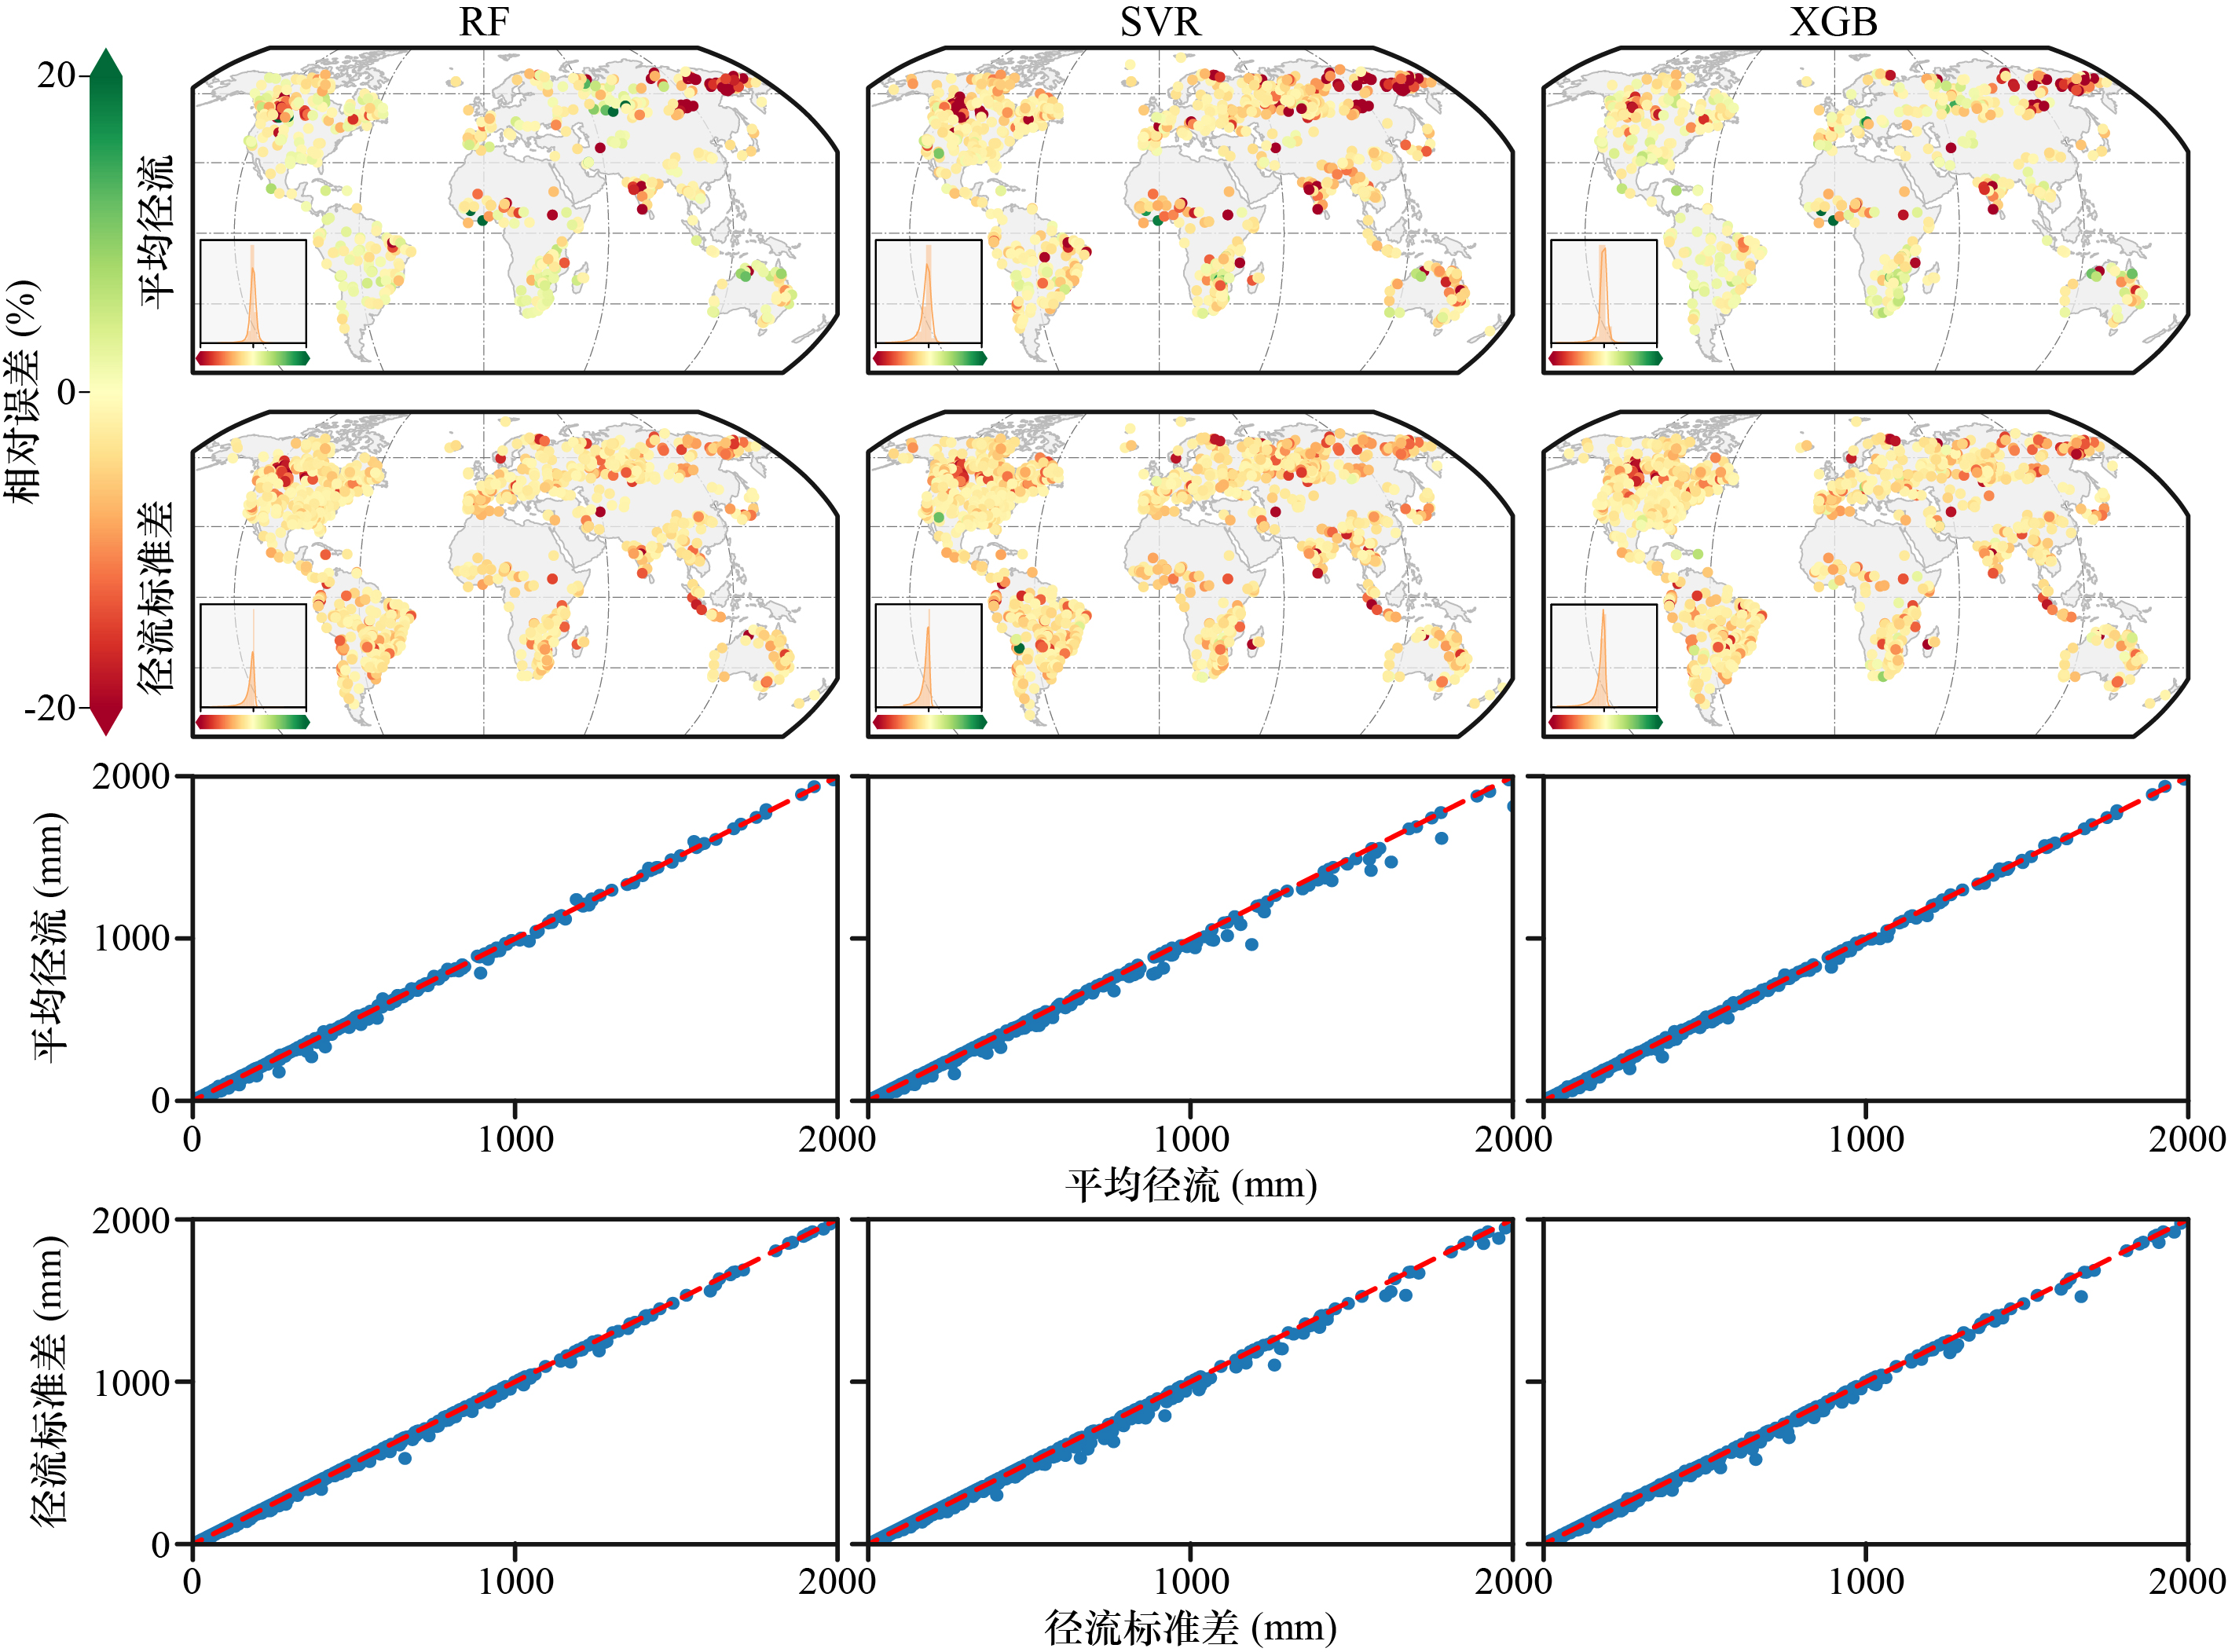
\includegraphics[width=0.9\textwidth]{figures/chap3/2_Interp_RE_Bef_Aft.jpg}
% 	\bicaption{数据插补前后径流量的相对误差和标准差的相对误差}{Relative error of runoff standard deviation between before and after the interpolation}
%   \label{fig:Interp_RE_Bef_Aft}
% \end{figure}

% \subsection{径流历史序列断点特征}

% \begin{figure}[H]
% 	\centering
% 	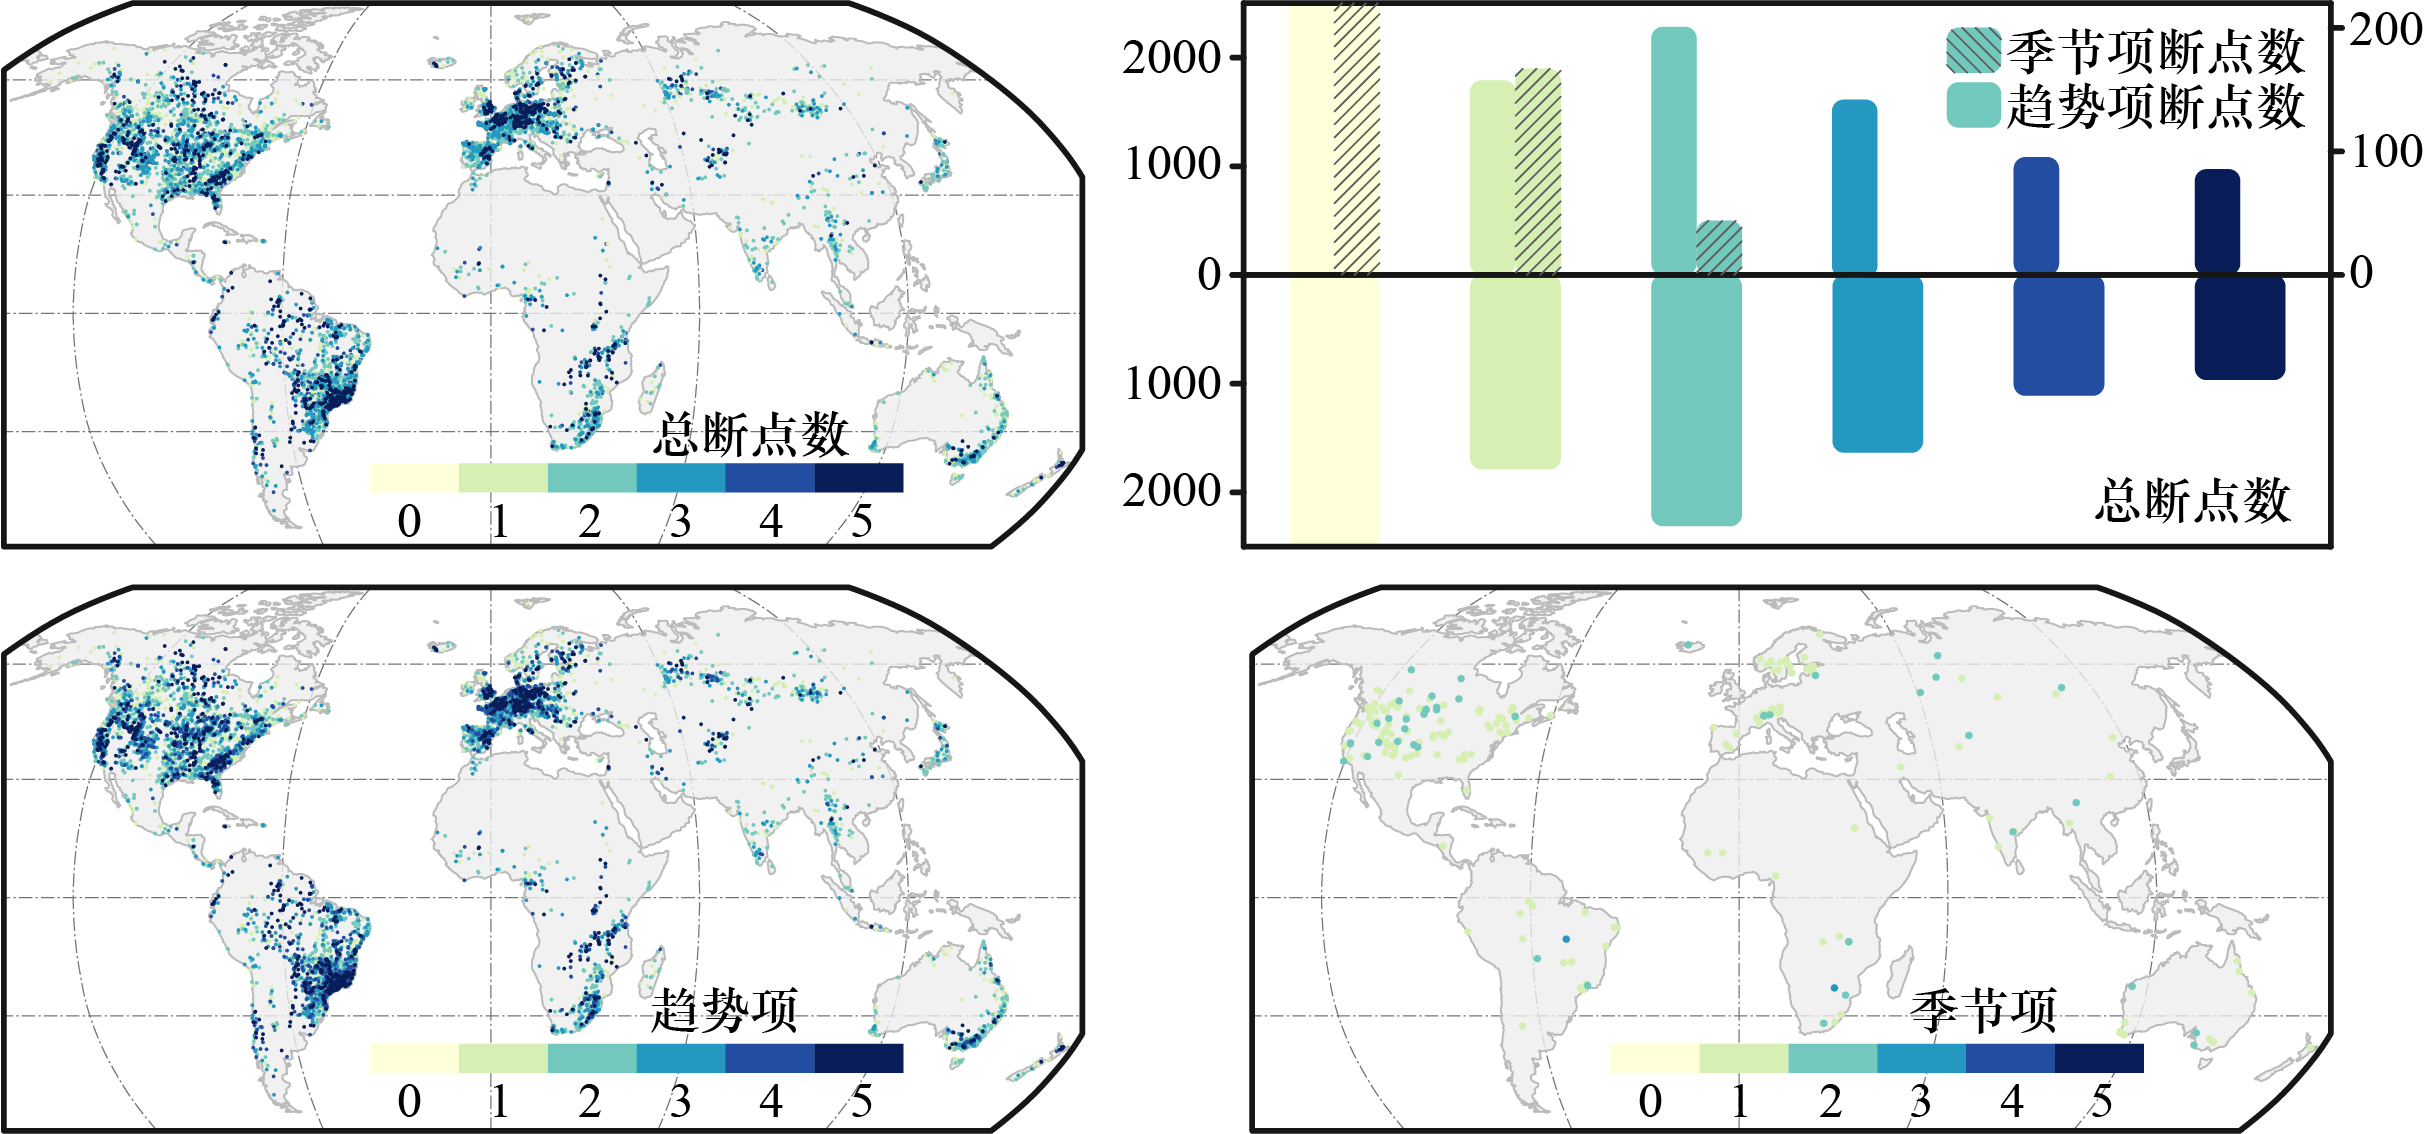
\includegraphics[width=0.8\textwidth]{figures/chap3/3_RUN_BP_Num.jpg}
% 	\bicaption{全球历史径流序列断点数量}{Breakpoints number in global historical runoff series}
%   \label{fig:RUN_BP_Num}
% \end{figure}

% \begin{figure}[H]
% 	\centering
% 	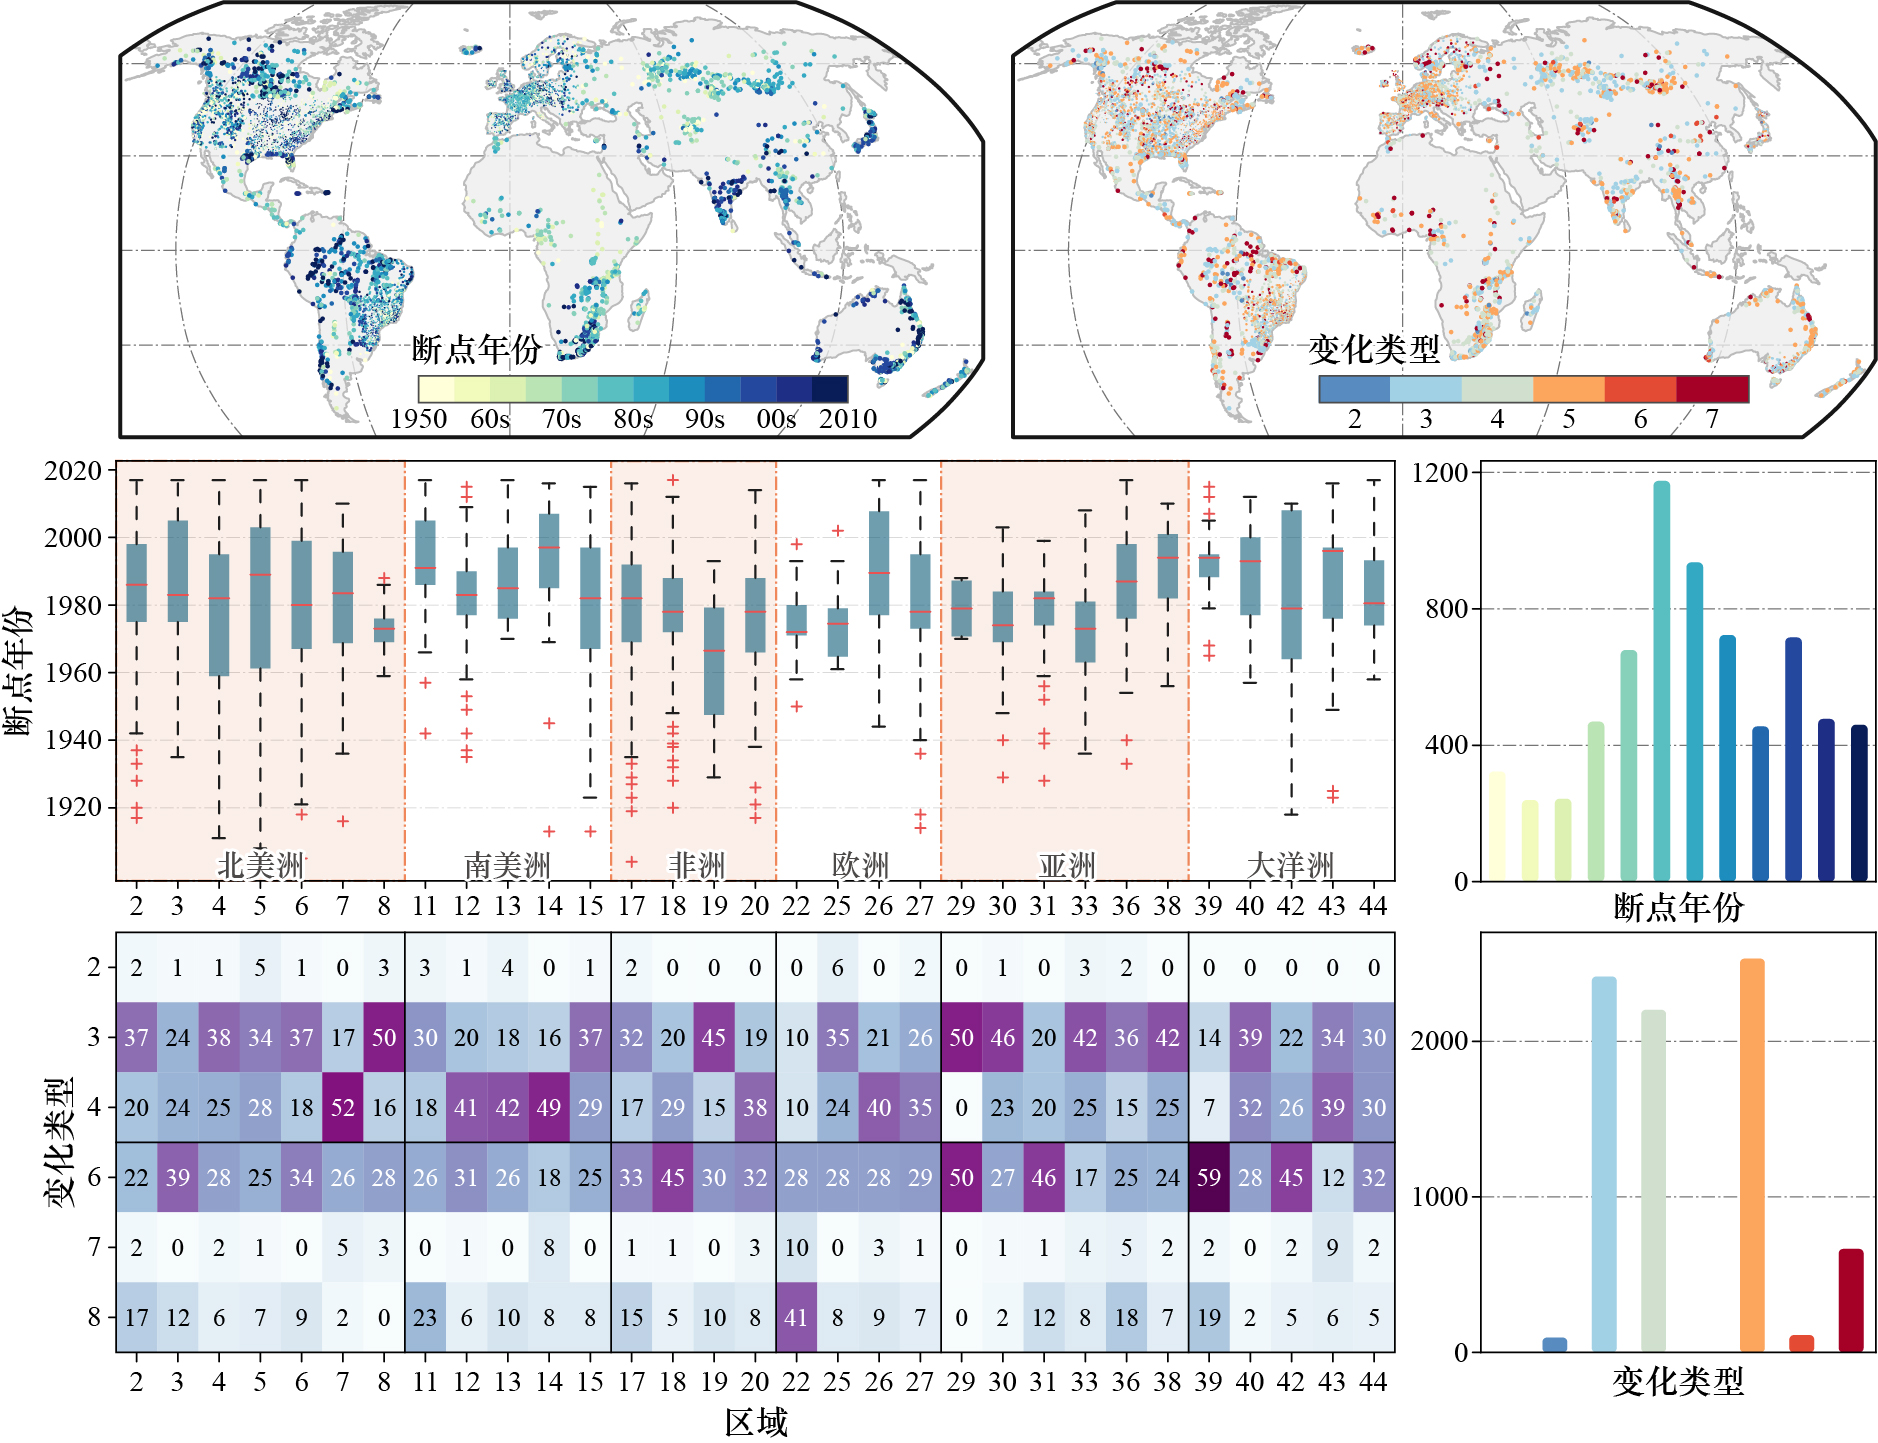
\includegraphics[width=0.9\textwidth]{figures/chap3/3_RUN_BT_Class.jpg}
% 	\bicaption{径流序列断点时间及序列变化特征}{Breakpoints time and change type before and after the breakpoint}
%   \label{fig:RUN_BT_Class}
% \end{figure}

% \subsection{全球陆地径流演变趋势}

% \section{多时空尺度径流变化归因分析}

% \section{讨论}

% \section{本章小结}

% \chapter{基于全球大样本的水量平衡模型基准测试}
\label{chap:model_compare}

\section{概述}

\section{研究方法}

\subsection{集总式水量平衡模型}

\subsection{参数率定方法}

\subsection{模型评价指标}

\subsection{实验设计}

\section{年、季尺度水量平衡模型基准测试}

\section{模型性能对流域水循环特征的响应}

\section{讨论}

\section{本章小结}

\clearpage
% \chapter{不确定性框架下的全球水量平衡模型构建}
\label{chap:params_regionalization}

\section{概述}

\section{研究方法}

\subsection{参数敏感性分析方法}

\subsection{模型参数不确定性分析方法}

\subsection{模型参数区域化方法}

\subsection{实验设计}

\section{参数敏感性分析结果}

\section{模型参数不确定性分析结果}

\section{全球水量平衡模型参数集}

\section{讨论}

\section{本章小结}

\clearpage
% \chapter{基于水量平衡的全球天然径流数据集}
\label{chap:model_compare}

\section{概述}

\section{研究方法}

\subsection{降尺度与偏差校正方法}

\subsection{长时间序列天然径流量估算方法}

\subsection{天然径流数据集评估方法}

\subsection{实验设计}

\section{全球气候模式数据降尺度结果评估}

\section{全球历史天然径流数据集构建与评估}

\section{全球未来水循环要素数据集构建与评估}

\section{讨论}

\section{本章小结}

\clearpage

%% 参考文献样式设定
\bibliographystyle{reference/hhuthesis-numeric}		% 顺序编码式
%% 参考文献,10号字,使用 BibTeX,包含参考文献文件.bib
% \bibliographystyle{reference/hhuthesis-numeric.bst} %
\bibliography{reference/thesis}

%%
%% 后置部分 
%% 

%% (其后部分无编号)
% \backmatter

%% 致谢
% \input{chapters/acknowledgement}

%% 附录
% \input{chapters/resume}

\end{document}
